\documentclass[twoside]{book}

% Packages required by doxygen
\usepackage{calc}
\usepackage{doxygen}
\usepackage{graphicx}
\usepackage[utf8]{inputenc}
\usepackage{makeidx}
\usepackage{multicol}
\usepackage{multirow}
\usepackage{textcomp}
\usepackage[table]{xcolor}

% Font selection
\usepackage[T1]{fontenc}
\usepackage{mathptmx}
\usepackage[scaled=.90]{helvet}
\usepackage{courier}
\usepackage{amssymb}
\usepackage{sectsty}
\renewcommand{\familydefault}{\sfdefault}
\allsectionsfont{%
  \fontseries{bc}\selectfont%
  \color{darkgray}%
}
\renewcommand{\DoxyLabelFont}{%
  \fontseries{bc}\selectfont%
  \color{darkgray}%
}

% Page & text layout
\usepackage{geometry}
\geometry{%
  a4paper,%
  top=2.5cm,%
  bottom=2.5cm,%
  left=2.5cm,%
  right=2.5cm%
}
\tolerance=750
\hfuzz=15pt
\hbadness=750
\setlength{\emergencystretch}{15pt}
\setlength{\parindent}{0cm}
\setlength{\parskip}{0.2cm}
\makeatletter
\renewcommand{\paragraph}{%
  \@startsection{paragraph}{4}{0ex}{-1.0ex}{1.0ex}{%
    \normalfont\normalsize\bfseries\SS@parafont%
  }%
}
\renewcommand{\subparagraph}{%
  \@startsection{subparagraph}{5}{0ex}{-1.0ex}{1.0ex}{%
    \normalfont\normalsize\bfseries\SS@subparafont%
  }%
}
\makeatother

% Headers & footers
\usepackage{fancyhdr}
\pagestyle{fancyplain}
\fancyhead[LE]{\fancyplain{}{\bfseries\thepage}}
\fancyhead[CE]{\fancyplain{}{}}
\fancyhead[RE]{\fancyplain{}{\bfseries\leftmark}}
\fancyhead[LO]{\fancyplain{}{\bfseries\rightmark}}
\fancyhead[CO]{\fancyplain{}{}}
\fancyhead[RO]{\fancyplain{}{\bfseries\thepage}}
\fancyfoot[LE]{\fancyplain{}{}}
\fancyfoot[CE]{\fancyplain{}{}}
\fancyfoot[RE]{\fancyplain{}{\bfseries\scriptsize Generated on Mon Jul 27 2015 16:16:49 for GAUSS Engine by Doxygen }}
\fancyfoot[LO]{\fancyplain{}{\bfseries\scriptsize Generated on Mon Jul 27 2015 16:16:49 for GAUSS Engine by Doxygen }}
\fancyfoot[CO]{\fancyplain{}{}}
\fancyfoot[RO]{\fancyplain{}{}}
\renewcommand{\footrulewidth}{0.4pt}
\renewcommand{\chaptermark}[1]{%
  \markboth{#1}{}%
}
\renewcommand{\sectionmark}[1]{%
  \markright{\thesection\ #1}%
}

% Indices & bibliography
\usepackage{natbib}
\usepackage[titles]{tocloft}
\setcounter{tocdepth}{3}
\setcounter{secnumdepth}{5}
\makeindex

% Hyperlinks (required, but should be loaded last)
\usepackage{ifpdf}
\ifpdf
  \usepackage[pdftex,pagebackref=true]{hyperref}
\else
  \usepackage[ps2pdf,pagebackref=true]{hyperref}
\fi
\hypersetup{%
  colorlinks=true,%
  linkcolor=blue,%
  citecolor=blue,%
  unicode%
}

% Custom commands
\newcommand{\clearemptydoublepage}{%
  \newpage{\pagestyle{empty}\cleardoublepage}%
}


%===== C O N T E N T S =====

\begin{document}

% Titlepage & ToC
\hypersetup{pageanchor=false}
\pagenumbering{roman}
\begin{titlepage}
\vspace*{7cm}
\begin{center}%
{\Large G\-A\-U\-S\-S Engine \\[1ex]\large 0.\-2 }\\
\vspace*{1cm}
{\large Generated by Doxygen 1.8.3.1-20130324}\\
\vspace*{0.5cm}
{\small Mon Jul 27 2015 16:16:49}\\
\end{center}
\end{titlepage}
\clearemptydoublepage
\tableofcontents
\clearemptydoublepage
\pagenumbering{arabic}
\hypersetup{pageanchor=true}

%--- Begin generated contents ---
\chapter{Main Page}
\label{index}\hypertarget{index}{}\hypertarget{index_intro_sec}{}\section{Introduction}\label{index_intro_sec}
Thank you for choosing the \hyperlink{class_g_a_u_s_s}{G\-A\-U\-S\-S} Engine A\-P\-I.

This library is a set of target language bindings that allows developers to intuitively and efficiently access the power of the \hyperlink{class_g_a_u_s_s}{G\-A\-U\-S\-S} Engine.

To accomplish the task of providing these bindings for multiple languages, we have created an initial C++ library and use the \href{http://www.swig.org}{\tt S\-W\-I\-G} program to generate language-\/specific bindings.

While building from source allows complete control over the compile process, we have elected to also release binaries for popular platforms.

You can easily and effectively\-:
\begin{DoxyItemize}
\item Create and destroy workspaces, using multiple for threaded situations
\item Compile, save, load and execute programs.
\item Manipulate data in the symbol table
\item Set up callbacks for integration with \hyperlink{class_g_a_u_s_s}{G\-A\-U\-S\-S}'s input/output routines
\end{DoxyItemize}\hypertarget{index_getting_started_sec}{}\section{Configuration}\label{index_getting_started_sec}
There are a few things necessary to take care of before starting development.

The A\-P\-I will look for the {\ttfamily M\-T\-E\-N\-G\-H\-O\-M\-E13} environment variable. This will be the location the engine was extracted to (i.\-e. {\ttfamily C\-:\textbackslash{}mteng13} on Windows, {\ttfamily /home/user/mteng13} on Linux)

\begin{TabularC}{2}
\hline
\rowcolor{lightgray}{\bf Variable }&{\bf Value}\\\cline{1-2}
{\ttfamily M\-T\-E\-N\-G\-H\-O\-M\-E13} &{\ttfamily /home/user/mteng13} \\\cline{1-2}
\end{TabularC}


The following environment variables must {\bfseries contain} the specified values\hypertarget{index_windows_install}{}\subsection{Windows}\label{index_windows_install}
\begin{TabularC}{2}
\hline
\rowcolor{lightgray}{\bf Variable }&{\bf Value}\\\cline{1-2}
{\ttfamily P\-A\-T\-H} &Append {\ttfamily C\-:\textbackslash{}mteng13} \\\cline{1-2}
\end{TabularC}


The presence of this value allows the engine D\-L\-L to be found and loaded properly.

Ensure you do not {\bfseries replace} {\ttfamily P\-A\-T\-H} with the directory.\hypertarget{index_linux_unix_install}{}\subsection{Linux and Unix}\label{index_linux_unix_install}
\begin{TabularC}{2}
\hline
\rowcolor{lightgray}{\bf Variable }&{\bf Value}\\\cline{1-2}
{\ttfamily L\-D\-\_\-\-L\-I\-B\-R\-A\-R\-Y\-\_\-\-P\-A\-T\-H} &Append {\ttfamily /home/user/mteng13} \\\cline{1-2}
{\ttfamily L\-D\-\_\-\-P\-R\-E\-L\-O\-A\-D} &Append {\ttfamily /lib/x86\-\_\-64-\/linux-\/gnu/libpthread.so.\-0\-:/home/user/mteng13/bin/libiomp5.so} \\\cline{1-2}
\end{TabularC}


Note\-: Please adjust the paths accordingly to your specific installation. In this case, the {\ttfamily libpthread.\-so.\-0} reference is for Ubuntu 64-\/bit.\hypertarget{index_swig_config}{}\subsection{S\-W\-I\-G}\label{index_swig_config}
If you are building from source, you will need to have the S\-W\-I\-G library available\-:

\href{http://www.swig.org/download.html}{\tt http\-://www.\-swig.\-org/download.\-html}

Once installed, please ensure {\ttfamily swig} is available in your terminal by placing it's installation directory in your {\ttfamily P\-A\-T\-H} environment variable, as building requires it.

{\bfseries E\-X\-C\-E\-P\-T\-I\-O\-N}\-: If you are not {\itshape modifying} any source files, the auto generated files have been included in the respective {\ttfamily python} and {\ttfamily php} sub-\/directories.

You can place these in {\ttfamily src} and skip the steps involving S\-W\-I\-G.\hypertarget{index_installation}{}\section{Installation}\label{index_installation}
This guide will not cover installation of the language itself. Please refer to the vendor documentation for language-\/level installation.\hypertarget{index_python_install}{}\subsection{Python}\label{index_python_install}
Installation of the Python module is fairly simple, since it uses the {\ttfamily distribute} package.\hypertarget{index_python_install_binary}{}\subsubsection{Binary}\label{index_python_install_binary}
\paragraph*{Windows}

Select the correct {\ttfamily egg} file according to your architecture.

Please ensure your Python installation contains the {\ttfamily setuptools} package, which provides the {\ttfamily easy\-\_\-install} application.

Instructions and files can be found at\-: \href{https://pypi.python.org/pypi/setuptools#windows}{\tt https\-://pypi.\-python.\-org/pypi/setuptools\#windows} \begin{DoxyVerb}$ easy_install gauss-0.1-py2.7-win-amd64.egg
\end{DoxyVerb}


\paragraph*{Linux}

\begin{DoxyVerb}$ easy_install gauss-0.1-py2.7-linux-x86_64.egg
\end{DoxyVerb}
\hypertarget{index_python_install_source}{}\subsubsection{Source}\label{index_python_install_source}
Due to the nature of the Python installation on Windows, please ensure the following are correctly in your {\ttfamily P\-A\-T\-H} environment variable \begin{DoxyVerb}C:\Python27\;C:\Python27\Scripts\
\end{DoxyVerb}


Note\-: Tested with Python 2.\-7.\-4

Since we are building from source, we need to run S\-W\-I\-G on our interface file.

This is done automatically with the {\ttfamily setup.\-py} file, however, we must first build the extension.

By first calling {\ttfamily build\-\_\-ext -\/i}, a {\ttfamily gauss.\-py} file is automatically generated in the current directory.

Subsequently calling the {\ttfamily install} target will now correctly install the files.

\paragraph*{Linux or Cygwin}


\begin{DoxyCode}
\textcolor{preprocessor}{# The setup.py utilizes the 'MTENGHOME13' environment variable.}
\textcolor{preprocessor}{}\textcolor{preprocessor}{# Please ensure this is set appropriately to your GAUSS Engine installation directory.}
\textcolor{preprocessor}{}tar -xvf gauss-0.1.tar.gz
cd gauss-0.1
python setup.py build\_ext -i      # First build the extension and create the gauss.py file
python setup.py install           # Everything compiled, now install

\textcolor{preprocessor}{# ROOT ONLY}
\textcolor{preprocessor}{}\textcolor{preprocessor}{# If installation must be done as root, force set the environment variable}
\textcolor{preprocessor}{}tar -xvf gauss-0.1.tar.gz
cd gauss-0.1
sudo MTENGHOME13=/home/user/mteng python setup.py build\_ext -i      # First build the extension and create 
      the gauss.py file
sudo MTENGHOME13=/home/user/mteng python setup.py install           # Everything compiled, now install
\end{DoxyCode}


\paragraph*{Windows}

Due to {\ttfamily mteng.\-dll} being compiled with V\-S 2008, it is necessary at this time to use M\-S\-V\-C to compile the Python extension.

All commands are run through the appropriate Visual Studio command prompt.

32-\/bit\-: {\ttfamily Start -\/$>$ Microsoft Visual Studio 2008 -\/$>$ Visual Studio Tools -\/$>$ Visual Studio 2008 Command Prompt}

64-\/bit\-: {\ttfamily Start -\/$>$ Microsoft Visual Studio 2008 -\/$>$ Visual Studio Tools -\/$>$ Visual Studio 2008 x64 Win64 Command Prompt}

If your user does have appropriate permissions to access the Python installation directory, you may have to run {\ttfamily cmd} as Administrator

Execute the following via a {\ttfamily cmd} terminal\-:


\begin{DoxyCode}
\textcolor{preprocessor}{# The setup.py utilizes the 'MTENGHOME13' environment variable.}
\textcolor{preprocessor}{}\textcolor{preprocessor}{# Please ensure this is set appropriately to your GAUSS Engine installation directory.}
\textcolor{preprocessor}{}\textcolor{preprocessor}{# unzip gauss-01.zip to a directory of your choice}
\textcolor{preprocessor}{}cd gauss-0.1
python setup.py build\_ext -i      # First build the extension and create the gauss.py file
python setup.py install           # Everything compiled, now install
\end{DoxyCode}


If you omit the {\ttfamily build\-\_\-ext -\/i} step, the {\ttfamily gauss.\-py} generated file will {\bfseries N\-O\-T} be placed in Python package directory.

The result of this behavior is the following when attempting to {\ttfamily import gauss}\-: \begin{DoxyVerb}>>> import gauss
Traceback (most recent call last):
  File "<stdin>", line 1, in <module>
ImportError: No module named gauss
\end{DoxyVerb}
\hypertarget{index_php_install}{}\subsection{P\-H\-P}\label{index_php_install}
\hypertarget{index_php_install_source}{}\subsubsection{Source}\label{index_php_install_source}
\href{http://www.cmake.org}{\tt C\-Make} is our build tool of choice. Get it.

There are a couple steps common between both platforms that should be done ahead of time.


\begin{DoxyEnumerate}
\item Set P\-H\-P specific environment variables.

Our C\-Make file uses the {\ttfamily P\-H\-P\-\_\-\-I\-N\-C\-L\-U\-D\-E} environment variable to locate P\-H\-P headers. It expects a semi-\/colon delimited list of paths.

For convenience, the Linux implementation does a string replace of '{\ttfamily -\/\-I}' with a semi-\/colon, so the following will work fine. \begin{DoxyVerb}# Linux
$ export PHP_INCLUDE=`php-config --includes`

# Windows you have to create it yourself. Newlines have been removed to clearly show the paths
# The actual command should have them all appended to each one another separated by a semi-colon
set PHP_INCLUDE=C:\development\php5.4ts\dev;
                C:\development\php-sdk\php54dev\vc9\x86\php-5.4.14-src;
                C:\development\php-sdk\php54dev\vc9\x86\php-5.4.14-src\main;
                C:\development\php-sdk\php54dev\vc9\x86\php-5.4.14-src\Zend;
                C:\development\php-sdk\php54dev\vc9\x86\php-5.4.14-src\TSRM;
                C:\development\php-sdk\php54dev\vc9\x86\php-5.4.14-src\ext
\end{DoxyVerb}


{\bfseries Note} the Windows line also has the {\ttfamily php5.\-4ts\textbackslash{}dev} as part of the include path.

This is so {\ttfamily php5ts.\-lib} can be located properly at link-\/time.
\item Execute S\-W\-I\-G manually (If you are using pre-\/generated files from the appropriate language's directory, you can skip this step)

Unlike our Python installation script, C\-Make does not automatically execute S\-W\-I\-G on the source files.

Run one directory up from {\ttfamily src}\-: \begin{DoxyVerb}swig -c++ -php -outdir src -o src/gauss_wrap.cpp gauss.i
\end{DoxyVerb}

\end{DoxyEnumerate}

After executing {\ttfamily swig}, you will find a newly created {\ttfamily gauss.\-php} in the {\ttfamily src} directory.

This will need to be used with any project that makes use of the \hyperlink{class_g_a_u_s_s}{G\-A\-U\-S\-S} Engine, as the first line of any program will be \begin{DoxyVerb}include("gauss.php");
\end{DoxyVerb}


\paragraph*{Linux}

The following commands are executed from the root of the source path \begin{DoxyVerb}$ mkdir build
$ cd build
# You could also use cmake-gui to create the Makefile
$ ccmake ..
$ make
\end{DoxyVerb}


You should now have a {\ttfamily gauss.\-so} file in your current directory.

Refer to the \href{#php_install_binary}{\tt P\-H\-P Binary} section for instructions on installation.

\paragraph*{Windows}

Currently, only compilation against P\-H\-P 5.\-4.\-14 (x86) {\itshape Thread Safe} version has been verified to work. Tested with Windows 7 Enterprise with Visual Studio 2008 S\-P1

{\bfseries Compile bug work-\/around\-:}

Per a bug report at, \href{https://bugs.php.net/bug.php?id=63130,}{\tt https\-://bugs.\-php.\-net/bug.\-php?id=63130,} and until a better solution is presented, you should make the following changes to {\ttfamily malloc.\-h}\-:

This is a possible path where you might find it\-: \begin{DoxyVerb}C:\Program Files (x86)\Microsoft Visual Studio 9.0\VC\include\malloc.h
\end{DoxyVerb}


open it up as Administrator and change


\begin{DoxyCode}
\textcolor{preprocessor}{#define \_STATIC\_ASSERT(expr) typedef char \_\_static\_assert\_t[ (expr) ]}
\end{DoxyCode}
 to 
\begin{DoxyCode}
\textcolor{preprocessor}{#ifdef PHP\_WIN32}
\textcolor{preprocessor}{}\textcolor{preprocessor}{#define \_STATIC\_ASSERT(expr) typedef char \_\_static\_assert\_t[ 1 ]}
\textcolor{preprocessor}{}\textcolor{preprocessor}{#else}
\textcolor{preprocessor}{}\textcolor{preprocessor}{#define \_STATIC\_ASSERT(expr) typedef char \_\_static\_assert\_t[ (expr) ]}
\textcolor{preprocessor}{#endif}
\end{DoxyCode}


Run the {\ttfamily cmake-\/gui} utility to configure and generate the V\-S Solution or N\-Make Makefile.

I chose to specify {\ttfamily build} as the directory for output.

If all went well, building the solution should now provide a {\ttfamily php\-\_\-gauss.\-dll} file in the {\ttfamily build\textbackslash{}Release} directory.\hypertarget{index_php_install_binary}{}\subsubsection{Binary}\label{index_php_install_binary}
\paragraph*{Windows / Linux}

Place the {\ttfamily php\-\_\-gauss.\-dll} (Windows) or {\ttfamily gauss.\-so} (Linux) in your P\-H\-P installation's {\ttfamily ext} directory.

This value can be found by either\-:


\begin{DoxyEnumerate}
\item {\ttfamily echo `php-\/config -\/-\/extension-\/dir`} on Linux
\item Looking for the {\ttfamily extension\-\_\-dir} value in your {\ttfamily php.\-ini} file.
\end{DoxyEnumerate}

There is also the opportunity to load the extension directly by P\-H\-P, requiring the addition of the following to your {\ttfamily php.\-ini}\-: \begin{DoxyVerb}; load gauss engine extension
; specify gauss.so if Linux
extension=php_gauss.dll
\end{DoxyVerb}


If running P\-H\-P from the command line, changes should be instantaneous.

Please refresh services that utilize P\-H\-P to pick up on the new extension.\hypertarget{index_example_apps}{}\section{Development}\label{index_example_apps}
This section introduces an implementation of the \hyperlink{class_g_a_u_s_s}{G\-A\-U\-S\-S} Engine.\hypertarget{index_hello_world}{}\subsection{Hello World!}\label{index_hello_world}
Getting started with the \hyperlink{class_g_a_u_s_s}{G\-A\-U\-S\-S} Engine is extremely simple.

This assumes the library has been made available to the target language properly.

The following snippet will be described step-\/by-\/step in detail\-:

\paragraph*{Python}


\begin{DoxyCode}
1 \textcolor{keyword}{from} gauss \textcolor{keyword}{import} GAUSS, IGEProgramOutput
2 
3 \textcolor{keyword}{class }Output(\hyperlink{class_i_g_e_program_output}{IGEProgramOutput}):
4     \textcolor{keyword}{def }invoke(self, message):
5         \textcolor{keywordflow}{print} message,
6 
7 ge = \hyperlink{class_g_a_u_s_s}{GAUSS}()
8 
9 out = Output()
10 out.thisown = 0
11 ge.setProgramOutputAll(out)
12 
13 \textcolor{keywordflow}{if} \textcolor{keywordflow}{not} ge.initialize():
14     \textcolor{keywordflow}{print} \textcolor{stringliteral}{"Initialization failed."}
15     sys.exit(1)     \textcolor{comment}{# import sys for usage}
16 
17 ge.executeString(\textcolor{stringliteral}{"print \(\backslash\)"Hello World!\(\backslash\)""})
18 ge.shutdown()
\end{DoxyCode}


\paragraph*{P\-H\-P}


\begin{DoxyCode}
include(\textcolor{stringliteral}{"gauss.php"});

\textcolor{keyword}{class }Output \textcolor{keyword}{extends} \hyperlink{class_i_g_e_program_output}{IGEProgramOutput} \{
    \textcolor{keyword}{function} invoke($message) \{
        echo $message;
    \}
\}

$ge = \textcolor{keyword}{new} \hyperlink{class_g_a_u_s_s}{GAUSS}();

$out = \textcolor{keyword}{new} Output();
$out->thisown = 0;

$ge->setProgramOutputAll($out);

\textcolor{keywordflow}{if} (!$ge->initialize()) \{
    echo \textcolor{stringliteral}{"Initialization failed."};
    \textcolor{keywordflow}{return};
\}

$ge->executeString(\textcolor{stringliteral}{"print \(\backslash\)"Hello World!\(\backslash\)""});
$ge->shutdown();
\end{DoxyCode}
\hypertarget{index_hw_step1}{}\subsection{Step 1\-: Import the required library}\label{index_hw_step1}
Before we can make use of the functionality, we have to make the engine library available to us. This is quite simple and straight-\/forward.

\paragraph*{Python}


\begin{DoxyCode}
1 \textcolor{keyword}{from} gauss \textcolor{keyword}{import} GAUSS, IGEProgramOutput
\end{DoxyCode}


\paragraph*{P\-H\-P}


\begin{DoxyCode}
include(\textcolor{stringliteral}{"gauss.php"});
\end{DoxyCode}


If you compiled from source and you're not sure where {\ttfamily gauss.\-php} is, recall that S\-W\-I\-G auto-\/generated it for us and it should be in the {\ttfamily src} directory.\hypertarget{index_hw_step2}{}\subsection{Step 2\-: Instantiate the G\-A\-U\-S\-S Engine object}\label{index_hw_step2}
After importing the correct library, we need to instantiate our engine object. There are multiple constructors available that suit a variety of scenarios.

In this example, we will be using the default constructor. This method relies on an existing environment variable in an effort to locate the \hyperlink{class_g_a_u_s_s}{G\-A\-U\-S\-S} home directory.

By default, this environment variable is {\ttfamily M\-T\-E\-N\-G\-H\-O\-M\-E13}.

\paragraph*{Python}


\begin{DoxyCode}
1 ge = \hyperlink{class_g_a_u_s_s}{GAUSS}()  \textcolor{comment}{# Look up value for MTENGHOME13}
\end{DoxyCode}
 \paragraph*{P\-H\-P}


\begin{DoxyCode}
$ge = \textcolor{keyword}{new} \hyperlink{class_g_a_u_s_s}{GAUSS}();  \textcolor{comment}{// Look up value for MTENGHOME13}
\end{DoxyCode}


{\bfseries Hint\-:} Check out the {\ttfamily G\-A\-U\-S\-S(string)} constructor, as it allows you to pass in a custom environment variable to use.\hypertarget{index_hw_step3}{}\subsection{Step 3\-: Set up callbacks}\label{index_hw_step3}
Technically, this step {\itshape can} be skipped, but creating appropriate callbacks allows you control over specific aspects of program functionality.

While some of these must be implemented to work correctly (i.\-e. setting a string input callback), others have default implementations that don't necessarily require a callback (i.\-e. program output routing to {\ttfamily stdout}), it is generally a good idea to do so.

The following 3 steps are core to setting up a callback\-:
\begin{DoxyEnumerate}
\item Define the callback by deriving one of the available callback classes
\item Set the {\ttfamily thisown} property to {\bfseries true} (release ownership)
\item Assign the callback
\end{DoxyEnumerate}

Pretty straight-\/forward!

We first define a callback class, inheriting the appropriate base class; in this case \hyperlink{class_i_g_e_program_output}{I\-G\-E\-Program\-Output}.

Simply override the callback method {\ttfamily invoke} and print out the {\ttfamily message} argument.

{\bfseries Important Note\-:}

We must set the {\ttfamily thisown} property of the newly instantiated object to {\ttfamily 0}

This is necessary because ownership of this object will be transferred to the \hyperlink{class_g_a_u_s_s}{G\-A\-U\-S\-S} object.

Without setting this, if the {\ttfamily out} var was to go out of scope, it could be deleted. When the engine attempts to clean up after itself, that object will no longer exist.

\paragraph*{Python}


\begin{DoxyCode}
1 \textcolor{comment}{# Step 1}
2 \textcolor{keyword}{class }Output(\hyperlink{class_i_g_e_program_output}{IGEProgramOutput}):
3     \textcolor{keyword}{def }invoke(self, message):
4         \textcolor{keywordflow}{print} message,
5 
6 out = Output()
7 
8 \textcolor{comment}{# Step 2}
9 out.thisown = 0 \textcolor{comment}{# Prevent garbage collection}
10 
11 \textcolor{comment}{# Step 3}
12 ge.setProgramOutputAll(out)
\end{DoxyCode}
 \paragraph*{P\-H\-P}


\begin{DoxyCode}
\textcolor{comment}{// Step 1}
\textcolor{keyword}{class }Output \textcolor{keyword}{extends} \hyperlink{class_i_g_e_program_output}{IGEProgramOutput} \{
    \textcolor{keyword}{function} invoke($message) \{
        echo $message;
    \}
\}

$out = \textcolor{keyword}{new} Output();

\textcolor{comment}{// Step 2}
$out->thisown = 0; \textcolor{comment}{// Prevent garbage collection}

\textcolor{comment}{// Step 3}
$ge->setProgramOutputAll($out);
\end{DoxyCode}


{\itshape Note\-:} We used the \hyperlink{class_g_a_u_s_s_a0b8379c48d677e05aeab433dba66fbb6}{G\-A\-U\-S\-S.\-set\-Program\-Output\-All} method, which is used to set {\itshape both} the program and error output.

If you wish to separate the callbacks for different functionality, you can use the \hyperlink{class_g_a_u_s_s_a7f0dc6b5b307aa06c347f9c6a9fdacab}{G\-A\-U\-S\-S.\-set\-Program\-Output} and \hyperlink{class_g_a_u_s_s_abd75266b2c4075da75163fe95b013ef3}{G\-A\-U\-S\-S.\-set\-Program\-Error\-Output} methods.\hypertarget{index_hw_step4}{}\subsection{Step 4\-: Initialize the G\-A\-U\-S\-S Engine}\label{index_hw_step4}
Now that you've made it to this step, if all has been configured correctly, initializing the Engine is quite easy.

\paragraph*{Python}


\begin{DoxyCode}
1 \textcolor{keywordflow}{if} \textcolor{keywordflow}{not} ge.initialize():
2     \textcolor{keywordflow}{print} \textcolor{stringliteral}{"Initialization failed."}
3     sys.exit(1)
\end{DoxyCode}
 \paragraph*{P\-H\-P}


\begin{DoxyCode}
\textcolor{keywordflow}{if} (!$ge->initialize()) \{
    echo \textcolor{stringliteral}{"Initialization failed."}
    \textcolor{keywordflow}{return};
\}
\end{DoxyCode}


The {\ttfamily initialize} method returns a true/false value depending on whether it was successful or not.\hypertarget{index_hw_step5}{}\subsection{Step 5\-: Home Free}\label{index_hw_step5}
With everything set up, we are free to run whatever code we choose!

For this small example, we just want the engine to tell us \char`\"{}\-Hello World!\char`\"{} through the callback we've assigned.

\paragraph*{Python}


\begin{DoxyCode}
1 ge.executeString(\textcolor{stringliteral}{"print \(\backslash\)"Hello World!\(\backslash\)""})
\end{DoxyCode}
 \paragraph*{P\-H\-P}


\begin{DoxyCode}
$ge->executeString(\textcolor{stringliteral}{"print \(\backslash\)"Hello World!\(\backslash\)""});
\end{DoxyCode}
 will result in the output\-: 
\begin{DoxyCode}
Hello World!
\end{DoxyCode}
\hypertarget{index_hw_step6}{}\subsection{Step 6\-: Shutdown the G\-A\-U\-S\-S Engine}\label{index_hw_step6}
Shutting down the \hyperlink{class_g_a_u_s_s}{G\-A\-U\-S\-S} Engine is as easy as telling it to do so\-:

\paragraph*{Python}


\begin{DoxyCode}
1 ge.shutdown()
\end{DoxyCode}
 \paragraph*{P\-H\-P}


\begin{DoxyCode}
$ge->shutdown();
\end{DoxyCode}


This will destroy any active workspaces and perform any cleanup that might be necessary.\hypertarget{index_conc}{}\subsection{Conclusion}\label{index_conc}
This wraps up the basics of using the \hyperlink{class_g_a_u_s_s}{G\-A\-U\-S\-S} Engine A\-P\-I. The documentation is full of code snippets that should help you easily interface with the Engine for your chosen task.

A template file has also been included which represents a full setup and tear-\/down with space in the middle to drop in code snippets. This file will be aptly named in relation to the language it applies to\-:

\begin{TabularC}{2}
\hline
\rowcolor{lightgray}{\bf Language }&{\bf Filename}\\\cline{1-2}
Python &{\ttfamily python/template\-\_\-example.\-py} \\\cline{1-2}
P\-H\-P &{\ttfamily php/template\-\_\-example.\-php} \\\cline{1-2}
\end{TabularC}

\chapter{Hierarchical Index}
\section{Class Hierarchy}
This inheritance list is sorted roughly, but not completely, alphabetically\-:\begin{DoxyCompactList}
\item \contentsline{section}{double\-Array}{\pageref{classdouble_array}}{}
\item \contentsline{section}{G\-A\-U\-S\-S}{\pageref{class_g_a_u_s_s}}{}
\item \contentsline{section}{G\-A\-U\-S\-S\-Private}{\pageref{class_g_a_u_s_s_private}}{}
\item \contentsline{section}{G\-E\-Symbol}{\pageref{class_g_e_symbol}}{}
\begin{DoxyCompactList}
\item \contentsline{section}{G\-E\-Array}{\pageref{class_g_e_array}}{}
\item \contentsline{section}{G\-E\-Matrix}{\pageref{class_g_e_matrix}}{}
\item \contentsline{section}{G\-E\-String\-Array}{\pageref{class_g_e_string_array}}{}
\end{DoxyCompactList}
\item \contentsline{section}{G\-E\-Sym\-Type\-\_\-s}{\pageref{struct_g_e_sym_type__s}}{}
\item \contentsline{section}{G\-E\-Workspace}{\pageref{class_g_e_workspace}}{}
\item \contentsline{section}{I\-G\-E\-Program\-Flush\-Output}{\pageref{class_i_g_e_program_flush_output}}{}
\item \contentsline{section}{I\-G\-E\-Program\-Input\-Char}{\pageref{class_i_g_e_program_input_char}}{}
\item \contentsline{section}{I\-G\-E\-Program\-Input\-Check}{\pageref{class_i_g_e_program_input_check}}{}
\item \contentsline{section}{I\-G\-E\-Program\-Input\-String}{\pageref{class_i_g_e_program_input_string}}{}
\item \contentsline{section}{I\-G\-E\-Program\-Output}{\pageref{class_i_g_e_program_output}}{}
\item \contentsline{section}{Workspace\-Manager}{\pageref{class_workspace_manager}}{}
\end{DoxyCompactList}

\chapter{Class Index}
\doxysection{Class List}
Here are the classes, structs, unions and interfaces with brief descriptions\+:\begin{DoxyCompactList}
\item\contentsline{section}{\mbox{\hyperlink{classdouble_array}{double\+Array}} }{\pageref{classdouble_array}}{}
\item\contentsline{section}{\mbox{\hyperlink{class_g_a_u_s_s}{GAUSS}} \\*Main class that must be instantiated to interface with the \mbox{\hyperlink{class_g_a_u_s_s}{GAUSS}} Engine }{\pageref{class_g_a_u_s_s}}{}
\item\contentsline{section}{\mbox{\hyperlink{class_g_a_u_s_s_private}{GAUSSPrivate}} }{\pageref{class_g_a_u_s_s_private}}{}
\item\contentsline{section}{\mbox{\hyperlink{class_g_e_array}{GEArray}} \\*\mbox{\hyperlink{class_g_a_u_s_s}{GAUSS}} Array symbol type }{\pageref{class_g_e_array}}{}
\item\contentsline{section}{\mbox{\hyperlink{class_g_e_matrix}{GEMatrix}} \\*\mbox{\hyperlink{class_g_a_u_s_s}{GAUSS}} Matrix symbol type }{\pageref{class_g_e_matrix}}{}
\item\contentsline{section}{\mbox{\hyperlink{class_g_e_string_array}{GEString\+Array}} \\*\mbox{\hyperlink{class_g_a_u_s_s}{GAUSS}} String Array Symbol type }{\pageref{class_g_e_string_array}}{}
\item\contentsline{section}{\mbox{\hyperlink{class_g_e_symbol}{GESymbol}} \\*Abstract parent class for all symbol types }{\pageref{class_g_e_symbol}}{}
\item\contentsline{section}{\mbox{\hyperlink{struct_g_e_sym_type__s}{GESym\+Type\+\_\+s}} \\*GESym\+Type stores \mbox{\hyperlink{class_g_a_u_s_s}{GAUSS}} constant values for different symbol types }{\pageref{struct_g_e_sym_type__s}}{}
\item\contentsline{section}{\mbox{\hyperlink{class_g_e_workspace}{GEWorkspace}} \\*Wrapper for a Workspace\+Handle\+\_\+t$\ast$ object }{\pageref{class_g_e_workspace}}{}
\item\contentsline{section}{\mbox{\hyperlink{class_i_g_e_program_flush_output}{IGEProgram\+Flush\+Output}} \\*Flush program output callback }{\pageref{class_i_g_e_program_flush_output}}{}
\item\contentsline{section}{\mbox{\hyperlink{class_i_g_e_program_input_char}{IGEProgram\+Input\+Char}} \\*Character input callback function for the \mbox{\hyperlink{class_g_a_u_s_s}{GAUSS}} Engine }{\pageref{class_i_g_e_program_input_char}}{}
\item\contentsline{section}{\mbox{\hyperlink{class_i_g_e_program_input_check}{IGEProgram\+Input\+Check}} \\*Input check callback function for the \mbox{\hyperlink{class_g_a_u_s_s}{GAUSS}} Engine }{\pageref{class_i_g_e_program_input_check}}{}
\item\contentsline{section}{\mbox{\hyperlink{class_i_g_e_program_input_string}{IGEProgram\+Input\+String}} \\*String Input callback function for the \mbox{\hyperlink{class_g_a_u_s_s}{GAUSS}} Engine }{\pageref{class_i_g_e_program_input_string}}{}
\item\contentsline{section}{\mbox{\hyperlink{class_i_g_e_program_output}{IGEProgram\+Output}} \\*This is the callback function that \mbox{\hyperlink{class_g_a_u_s_s}{GAUSS}} will call to do normal program output }{\pageref{class_i_g_e_program_output}}{}
\item\contentsline{section}{\mbox{\hyperlink{class_workspace_manager}{Workspace\+Manager}} }{\pageref{class_workspace_manager}}{}
\end{DoxyCompactList}

\chapter{Class Documentation}
\hypertarget{class_g_a_u_s_s}{\section{G\-A\-U\-S\-S Class Reference}
\label{class_g_a_u_s_s}\index{G\-A\-U\-S\-S@{G\-A\-U\-S\-S}}
}


Main class that must be instantiated to interface with the \hyperlink{class_g_a_u_s_s}{G\-A\-U\-S\-S} Engine.  




{\ttfamily \#include $<$gauss.\-h$>$}

\subsection*{Public Member Functions}
\begin{DoxyCompactItemize}
\item 
\hyperlink{class_g_a_u_s_s_aba6a26957e7dbcd8f6357d1ca6ff4b90}{G\-A\-U\-S\-S} (void)
\begin{DoxyCompactList}\small\item\em Initialize the library using the environment variable value of {\ttfamily M\-T\-E\-N\-G\-H\-O\-M\-E13} as the path for the \hyperlink{class_g_a_u_s_s}{G\-A\-U\-S\-S} Home path. \end{DoxyCompactList}\item 
\hyperlink{class_g_a_u_s_s_afd3a4f159bc887697d0dc6f1781714ae}{G\-A\-U\-S\-S} (string, bool is\-Env\-Var=true)
\begin{DoxyCompactList}\small\item\em Initialize the library using the specified environment variable that contains the path for the \hyperlink{class_g_a_u_s_s}{G\-A\-U\-S\-S} Home directory. \end{DoxyCompactList}\item 
bool \hyperlink{class_g_a_u_s_s_aad9f7a3a527b9c5961d1cc1b1aa9066c}{initialize} ()
\begin{DoxyCompactList}\small\item\em Initialize the \hyperlink{class_g_a_u_s_s}{G\-A\-U\-S\-S} Engine. \end{DoxyCompactList}\item 
void \hyperlink{class_g_a_u_s_s_a71721c595c12c94616ef414879c95460}{shutdown} ()
\begin{DoxyCompactList}\small\item\em Free all created workspaces and shut down the \hyperlink{class_g_a_u_s_s}{G\-A\-U\-S\-S} Engine. \end{DoxyCompactList}\item 
bool \hyperlink{class_g_a_u_s_s_af1f5a5df0c904bd713c4edea74606e55}{set\-Home} (string)
\begin{DoxyCompactList}\small\item\em Specifies the home directory used to locate the Run-\/\-Time Library, source files, library files, etc. \end{DoxyCompactList}\item 
bool \hyperlink{class_g_a_u_s_s_a61b2ebc8c6ac5694e8cc33cb7726cbe3}{set\-Home\-Var} (string)
\begin{DoxyCompactList}\small\item\em The default value is {\ttfamily M\-T\-E\-N\-G\-H\-O\-M\-E\#\#}. \end{DoxyCompactList}\item 
string \hyperlink{class_g_a_u_s_s_adfe744665cc891f5288d5523083d2a2c}{get\-Home} ()
\begin{DoxyCompactList}\small\item\em Returns the current path known by the \hyperlink{class_g_a_u_s_s}{G\-A\-U\-S\-S} Engine for the user home directory. \end{DoxyCompactList}\item 
string \hyperlink{class_g_a_u_s_s_abb13d8fd5b2abd2844e48279621204e6}{get\-Home\-Var} ()
\begin{DoxyCompactList}\small\item\em Returns the current environment variable value set by the \hyperlink{class_g_a_u_s_s}{G\-A\-U\-S\-S} Engine that represents the \hyperlink{class_g_a_u_s_s}{G\-A\-U\-S\-S} Home path. \end{DoxyCompactList}\item 
string \hyperlink{class_g_a_u_s_s_ad9c991ab9fd7dea25a865eb1deae9b4c}{get\-Log\-File} ()
\begin{DoxyCompactList}\small\item\em Returns the current log file location used by the \hyperlink{class_g_a_u_s_s}{G\-A\-U\-S\-S} Engine. \end{DoxyCompactList}\item 
bool \hyperlink{class_g_a_u_s_s_a59f4b84f55f76701ca9deb7be3f9f0fe}{set\-Log\-File} (string, string)
\begin{DoxyCompactList}\small\item\em Allows you to set the file that the errors will be logged in. \end{DoxyCompactList}\item 
string \hyperlink{class_g_a_u_s_s_a048aa287aa5d82638aff68f4d4cbec28}{get\-Last\-Error\-Text} ()
\begin{DoxyCompactList}\small\item\em Return the string error description of the last error code. \end{DoxyCompactList}\item 
string \hyperlink{class_g_a_u_s_s_a6e487c8dc379177510f76e322b0e50de}{get\-Error\-Text} (int)
\begin{DoxyCompactList}\small\item\em Given a \hyperlink{class_g_a_u_s_s}{G\-A\-U\-S\-S} error code, return the full error description. \end{DoxyCompactList}\item 
int \hyperlink{class_g_a_u_s_s_a6a62cfdb5ea03e0352c271c60afe96fc}{get\-Error} ()
\begin{DoxyCompactList}\small\item\em Retrieve the last error code set by the \hyperlink{class_g_a_u_s_s}{G\-A\-U\-S\-S} Engine. \end{DoxyCompactList}\item 
void \hyperlink{class_g_a_u_s_s_a4adc9a33b8be97b1a6592160fea4a4eb}{set\-Error} (int)
\begin{DoxyCompactList}\small\item\em Manually set the current error code for the \hyperlink{class_g_a_u_s_s}{G\-A\-U\-S\-S} Engine. \end{DoxyCompactList}\item 
\hyperlink{class_g_e_workspace}{G\-E\-Workspace} $\ast$ \hyperlink{class_g_a_u_s_s_aa300ef0a2a359b736734b4350706ef89}{create\-Workspace} (string)
\begin{DoxyCompactList}\small\item\em Creates a new workspace with the given name, and returns a handle to it. \end{DoxyCompactList}\item 
bool \hyperlink{class_g_a_u_s_s_a22e8b7eebcc1e77708a7cfd9a858e769}{destroy\-Workspace} (\hyperlink{class_g_e_workspace}{G\-E\-Workspace} $\ast$)
\begin{DoxyCompactList}\small\item\em Free a workspace. \end{DoxyCompactList}\item 
void \hyperlink{class_g_a_u_s_s_ab9515a6de5028f18138e6c87e1512c91}{destroy\-All\-Workspaces} ()
\begin{DoxyCompactList}\small\item\em Clears all workspaces. \end{DoxyCompactList}\item 
\hyperlink{class_g_e_workspace}{G\-E\-Workspace} $\ast$ \hyperlink{class_g_a_u_s_s_a5d3dc85b8f31111c6bf3a2d8286c915e}{get\-Workspace} (string)
\begin{DoxyCompactList}\small\item\em Returns a handle to a specified workspace by {\itshape name} \end{DoxyCompactList}\item 
\hyperlink{class_g_e_workspace}{G\-E\-Workspace} $\ast$ \hyperlink{class_g_a_u_s_s_a566a50d644d0d1f55dba90416de4961a}{get\-Active\-Workspace} ()
\begin{DoxyCompactList}\small\item\em Return a handle to the currently active workspace. \end{DoxyCompactList}\item 
bool \hyperlink{class_g_a_u_s_s_a7ff4b1140967c6737918728227fa1419}{set\-Active\-Workspace} (\hyperlink{class_g_e_workspace}{G\-E\-Workspace} $\ast$)
\begin{DoxyCompactList}\small\item\em Sets the active workspace to be the specified workspace. \end{DoxyCompactList}\item 
\hyperlink{class_g_e_workspace}{G\-E\-Workspace} $\ast$ \hyperlink{class_g_a_u_s_s_a294a07247f6c7d8464ce5e79a97025a3}{load\-Workspace} (string)
\begin{DoxyCompactList}\small\item\em Gets the workspace information saved in a file and returns it in a workspace handle. \end{DoxyCompactList}\item 
string \hyperlink{class_g_a_u_s_s_aec6202efa12949e7a7e9addfedbc3ded}{get\-Workspace\-Name} (\hyperlink{class_g_e_workspace}{G\-E\-Workspace} $\ast$)
\begin{DoxyCompactList}\small\item\em Returns the current associated name of a workspace according to \hyperlink{class_g_a_u_s_s}{G\-A\-U\-S\-S}. \end{DoxyCompactList}\item 
void \hyperlink{class_g_a_u_s_s_a626d736a417fd10e0b51087e944c5e56}{update\-Workspace\-Name} (\hyperlink{class_g_e_workspace}{G\-E\-Workspace} $\ast$)
\begin{DoxyCompactList}\small\item\em Request the workspace name from \hyperlink{class_g_a_u_s_s}{G\-A\-U\-S\-S}, and set the {\itshape name} field in the \hyperlink{class_g_e_workspace}{G\-E\-Workspace} object. \end{DoxyCompactList}\item 
bool \hyperlink{class_g_a_u_s_s_acc7a8039355ae28686d9393144b2af75}{save\-Workspace} (\hyperlink{class_g_e_workspace}{G\-E\-Workspace} $\ast$, string)
\begin{DoxyCompactList}\small\item\em Saves workspace information contained in a workspace handle into a file. \end{DoxyCompactList}\item 
bool \hyperlink{class_g_a_u_s_s_af6c2bb49b3906debb760e103cc1436f9}{save\-Program} (Program\-Handle\-\_\-t $\ast$, string)
\begin{DoxyCompactList}\small\item\em Saves a compiled program given by a program handle into a file. \end{DoxyCompactList}\item 
string \hyperlink{class_g_a_u_s_s_a7403bd9564a21a81f790e88da97ff780}{translate\-Dataloop\-File} (string srcfile)
\begin{DoxyCompactList}\small\item\em Translates a file that contains a dataloop, so it can be read by the compiler. \end{DoxyCompactList}\item 
bool \hyperlink{class_g_a_u_s_s_a5e936488bfa9422a6267afbe7ab8ffe2}{execute\-String} (string)
\begin{DoxyCompactList}\small\item\em Executes a command within the \hyperlink{class_g_a_u_s_s}{G\-A\-U\-S\-S} Engine on the currently active workspace. \end{DoxyCompactList}\item 
bool \hyperlink{class_g_a_u_s_s_a32f1488454a0ee5522626fc8d322fea1}{execute\-String} (string, \hyperlink{class_g_e_workspace}{G\-E\-Workspace} $\ast$)
\begin{DoxyCompactList}\small\item\em Executes a command within the \hyperlink{class_g_a_u_s_s}{G\-A\-U\-S\-S} Engine on a specific workspace. \end{DoxyCompactList}\item 
bool \hyperlink{class_g_a_u_s_s_a1e15d3c30be612b67ecb67ed7a39b185}{execute\-File} (string)
\begin{DoxyCompactList}\small\item\em Executes a named file within the \hyperlink{class_g_a_u_s_s}{G\-A\-U\-S\-S} Engine on the currently active workspace. \end{DoxyCompactList}\item 
bool \hyperlink{class_g_a_u_s_s_aadc273c128c4d1fadb6edf0df7112107}{execute\-File} (string, \hyperlink{class_g_e_workspace}{G\-E\-Workspace} $\ast$)
\begin{DoxyCompactList}\small\item\em Executes a named file within the \hyperlink{class_g_a_u_s_s}{G\-A\-U\-S\-S} Engine on the a specific workspace. \end{DoxyCompactList}\item 
bool \hyperlink{class_g_a_u_s_s_a1b971703024494d1390241b86099ddbb}{execute\-Compiled\-File} (string)
\begin{DoxyCompactList}\small\item\em Executes a compiled gcg file within the \hyperlink{class_g_a_u_s_s}{G\-A\-U\-S\-S} Engine on the active workspace. \end{DoxyCompactList}\item 
bool \hyperlink{class_g_a_u_s_s_ad553ead84eec837e60782f16a3e242f8}{execute\-Compiled\-File} (string, \hyperlink{class_g_e_workspace}{G\-E\-Workspace} $\ast$)
\begin{DoxyCompactList}\small\item\em Executes a compiled gcg file within the \hyperlink{class_g_a_u_s_s}{G\-A\-U\-S\-S} Engine on a specific workspace. \end{DoxyCompactList}\item 
Program\-Handle\-\_\-t $\ast$ \hyperlink{class_g_a_u_s_s_a5062f8fabacaba21e242785a6461f9d1}{compile\-String} (string)
\begin{DoxyCompactList}\small\item\em Compiles a string and returns a program handle in the active workspace. \end{DoxyCompactList}\item 
Program\-Handle\-\_\-t $\ast$ \hyperlink{class_g_a_u_s_s_a13db047afc85a0ef2406b5e054bdea83}{compile\-String} (string, \hyperlink{class_g_e_workspace}{G\-E\-Workspace} $\ast$)
\begin{DoxyCompactList}\small\item\em Compiles a string and returns a program handle in the specified workspace. \end{DoxyCompactList}\item 
Program\-Handle\-\_\-t $\ast$ \hyperlink{class_g_a_u_s_s_a182412bc30b9750b57de41d2334470de}{compile\-File} (string)
\begin{DoxyCompactList}\small\item\em Compiles a file and returns a program handle in the active workspace. \end{DoxyCompactList}\item 
Program\-Handle\-\_\-t $\ast$ \hyperlink{class_g_a_u_s_s_ab26d63e1aa776415ec71166705a98664}{compile\-File} (string, \hyperlink{class_g_e_workspace}{G\-E\-Workspace} $\ast$)
\begin{DoxyCompactList}\small\item\em Compiles a file and returns a program handle in a specific workspace. \end{DoxyCompactList}\item 
Program\-Handle\-\_\-t $\ast$ \hyperlink{class_g_a_u_s_s_ae05e76794c7c581efa1fb38e6a94652f}{load\-Compiled\-File} (string)
\begin{DoxyCompactList}\small\item\em Loads an already compiled file into the active workspace and returns a program handle. \end{DoxyCompactList}\item 
Program\-Handle\-\_\-t $\ast$ \hyperlink{class_g_a_u_s_s_a7609366538fd9b85e3fa85a4b9b7bdb7}{load\-Compiled\-File} (string, \hyperlink{class_g_e_workspace}{G\-E\-Workspace} $\ast$)
\begin{DoxyCompactList}\small\item\em Loads an already compiled file into a specific workspace and returns a program handle. \end{DoxyCompactList}\item 
bool \hyperlink{class_g_a_u_s_s_ad680244c55b1d32cba04ab95a6572862}{execute\-Program} (Program\-Handle\-\_\-t $\ast$)
\begin{DoxyCompactList}\small\item\em Executes a given program handle that was created with either \hyperlink{class_g_a_u_s_s_a5062f8fabacaba21e242785a6461f9d1}{compile\-String(string)}, \hyperlink{class_g_a_u_s_s_a182412bc30b9750b57de41d2334470de}{compile\-File(string)}, or \hyperlink{class_g_a_u_s_s_ae05e76794c7c581efa1fb38e6a94652f}{load\-Compiled\-File(string)}. \end{DoxyCompactList}\item 
void \hyperlink{class_g_a_u_s_s_a626ad1e9228347c6b0d56b2b41337586}{free\-Program} (Program\-Handle\-\_\-t $\ast$)
\begin{DoxyCompactList}\small\item\em Free a program handle created by \hyperlink{class_g_a_u_s_s_a5062f8fabacaba21e242785a6461f9d1}{compile\-String(string)}, \hyperlink{class_g_a_u_s_s_a182412bc30b9750b57de41d2334470de}{compile\-File(string)}, and \hyperlink{class_g_a_u_s_s_ae05e76794c7c581efa1fb38e6a94652f}{load\-Compiled\-File(string)} \end{DoxyCompactList}\item 
string \hyperlink{class_g_a_u_s_s_a9b74886bf0091ca9d5bd17feae95ea05}{make\-Path\-Absolute} (string)
\begin{DoxyCompactList}\small\item\em Turns a given path into an absolute path. \end{DoxyCompactList}\item 
string \hyperlink{class_g_a_u_s_s_a7e1284a1d44e68aadb6c70e4416abb7b}{program\-Input\-String} ()
\begin{DoxyCompactList}\small\item\em Calls the program input string function hooked with \hyperlink{class_g_a_u_s_s_ae82b5bfdf26971433c46936a812506c3}{set\-Program\-Input\-String(\-I\-G\-E\-Program\-Input\-String$\ast$)}. \end{DoxyCompactList}\item 
int \hyperlink{class_g_a_u_s_s_aadbb588e6cb82219df8571ea17027d3c}{get\-Symbol\-Type} (string)
\begin{DoxyCompactList}\small\item\em Returns the type of a symbol in the active \hyperlink{class_g_a_u_s_s}{G\-A\-U\-S\-S} workspace or 0 if it cannot find the symbol. \end{DoxyCompactList}\item 
int \hyperlink{class_g_a_u_s_s_abc7d671bcf6ae784070a78bae1546f7a}{get\-Symbol\-Type} (string, \hyperlink{class_g_e_workspace}{G\-E\-Workspace} $\ast$)
\begin{DoxyCompactList}\small\item\em Returns the type of a symbol in a \hyperlink{class_g_a_u_s_s}{G\-A\-U\-S\-S} workspace or 0 if it cannot find the symbol. \end{DoxyCompactList}\item 
double \hyperlink{class_g_a_u_s_s_a7c44bea0167fd88360b3926904a5cf2f}{get\-Scalar} (string)
\begin{DoxyCompactList}\small\item\em Returns a scalar from the current workspace as a primitive {\ttfamily double}. \end{DoxyCompactList}\item 
double \hyperlink{class_g_a_u_s_s_ade5065d7eec4f6170496571a07e5dc4c}{get\-Scalar} (string, \hyperlink{class_g_e_workspace}{G\-E\-Workspace} $\ast$)
\begin{DoxyCompactList}\small\item\em Returns a scalar from a specific workspace as a primitive {\ttfamily double}. \end{DoxyCompactList}\item 
\hyperlink{class_g_e_matrix}{G\-E\-Matrix} $\ast$ \hyperlink{class_g_a_u_s_s_a7c2716d0bb1c2cdca5de3f74b89f045a}{get\-Matrix} (string)
\begin{DoxyCompactList}\small\item\em Retrieve a matrix from the \hyperlink{class_g_a_u_s_s}{G\-A\-U\-S\-S} symbol name in the active workspace. \end{DoxyCompactList}\item 
\hyperlink{class_g_e_matrix}{G\-E\-Matrix} $\ast$ \hyperlink{class_g_a_u_s_s_a760da892985076d0f595da7eb88a07fe}{get\-Matrix} (string, \hyperlink{class_g_e_workspace}{G\-E\-Workspace} $\ast$)
\begin{DoxyCompactList}\small\item\em Retrieve a matrix from the \hyperlink{class_g_a_u_s_s}{G\-A\-U\-S\-S} symbol name in workspace {\itshape wh}. \end{DoxyCompactList}\item 
\hyperlink{class_g_e_matrix}{G\-E\-Matrix} $\ast$ \hyperlink{class_g_a_u_s_s_ae015bd236952146aa33ed7e3a279ff04}{get\-Matrix\-And\-Clear} (string)
\begin{DoxyCompactList}\small\item\em Retrieve a matrix from the \hyperlink{class_g_a_u_s_s}{G\-A\-U\-S\-S} symbol name in the active workspace. \end{DoxyCompactList}\item 
\hyperlink{class_g_e_matrix}{G\-E\-Matrix} $\ast$ \hyperlink{class_g_a_u_s_s_afdb5633bee38528f3a19ec92b5d9b2a5}{get\-Matrix\-And\-Clear} (string, \hyperlink{class_g_e_workspace}{G\-E\-Workspace} $\ast$)
\begin{DoxyCompactList}\small\item\em Retrieve a matrix from the \hyperlink{class_g_a_u_s_s}{G\-A\-U\-S\-S} symbol name in workspace {\itshape wh}. \end{DoxyCompactList}\item 
\hyperlink{class_g_e_array}{G\-E\-Array} $\ast$ \hyperlink{class_g_a_u_s_s_a4016aa13feb5c5648556dcca73caf030}{get\-Array} (string)
\begin{DoxyCompactList}\small\item\em Retrieve an array from the \hyperlink{class_g_a_u_s_s}{G\-A\-U\-S\-S} symbol table in the active workspace. \end{DoxyCompactList}\item 
\hyperlink{class_g_e_array}{G\-E\-Array} $\ast$ \hyperlink{class_g_a_u_s_s_ac674a4f382ee80691146d412c3182c1d}{get\-Array} (string, \hyperlink{class_g_e_workspace}{G\-E\-Workspace} $\ast$)
\begin{DoxyCompactList}\small\item\em Retrieve an array from the \hyperlink{class_g_a_u_s_s}{G\-A\-U\-S\-S} symbol table in workspace {\itshape wh}. \end{DoxyCompactList}\item 
\hyperlink{class_g_e_array}{G\-E\-Array} $\ast$ \hyperlink{class_g_a_u_s_s_ad2bcca793c43675ff937c8637ec3e3e3}{get\-Array\-And\-Clear} (string)
\begin{DoxyCompactList}\small\item\em Retrieve an array from the \hyperlink{class_g_a_u_s_s}{G\-A\-U\-S\-S} symbol table in the active workspace. \end{DoxyCompactList}\item 
\hyperlink{class_g_e_array}{G\-E\-Array} $\ast$ \hyperlink{class_g_a_u_s_s_a9773d66de682d40025edef5b372ab9b8}{get\-Array\-And\-Clear} (string, \hyperlink{class_g_e_workspace}{G\-E\-Workspace} $\ast$)
\begin{DoxyCompactList}\small\item\em Retrieve an array from the \hyperlink{class_g_a_u_s_s}{G\-A\-U\-S\-S} symbol table in workspace {\itshape wh}. \end{DoxyCompactList}\item 
\hyperlink{class_g_e_string}{G\-E\-String} $\ast$ \hyperlink{class_g_a_u_s_s_ad75afe2cd19e141c15c97ad52373791d}{get\-String} (string)
\begin{DoxyCompactList}\small\item\em Retrieve a string from the \hyperlink{class_g_a_u_s_s}{G\-A\-U\-S\-S} symbol table in the active workspace. \end{DoxyCompactList}\item 
\hyperlink{class_g_e_string}{G\-E\-String} $\ast$ \hyperlink{class_g_a_u_s_s_a9b5d5caf2cc8932364a4a867c72b0854}{get\-String} (string, \hyperlink{class_g_e_workspace}{G\-E\-Workspace} $\ast$)
\begin{DoxyCompactList}\small\item\em Retrieve a string from the \hyperlink{class_g_a_u_s_s}{G\-A\-U\-S\-S} symbol table in workspace {\itshape wh}. \end{DoxyCompactList}\item 
\hyperlink{class_g_e_string_array}{G\-E\-String\-Array} $\ast$ \hyperlink{class_g_a_u_s_s_a9c1652bb6b3a931c75d9c7dd2ffe23cb}{get\-String\-Array} (string)
\begin{DoxyCompactList}\small\item\em Retrieve a string array from the \hyperlink{class_g_a_u_s_s}{G\-A\-U\-S\-S} symbol table in the active workspace. \end{DoxyCompactList}\item 
\hyperlink{class_g_e_string_array}{G\-E\-String\-Array} $\ast$ \hyperlink{class_g_a_u_s_s_aaec58da4530de9e471961a6ff0df79b5}{get\-String\-Array} (string, \hyperlink{class_g_e_workspace}{G\-E\-Workspace} $\ast$)
\begin{DoxyCompactList}\small\item\em Retrieve a string array from the \hyperlink{class_g_a_u_s_s}{G\-A\-U\-S\-S} symbol table in workspace {\itshape wh}. \end{DoxyCompactList}\item 
bool \hyperlink{class_g_a_u_s_s_ac3c631a4d751917f3dd5ec60e48ca908}{set\-Symbol} (\hyperlink{class_g_e_matrix}{G\-E\-Matrix} $\ast$, string)
\begin{DoxyCompactList}\small\item\em Add a matrix to the active workspace with the specified symbol name. \end{DoxyCompactList}\item 
bool \hyperlink{class_g_a_u_s_s_ab90cec0135942174b273fd5c258b9740}{set\-Symbol} (\hyperlink{class_g_e_matrix}{G\-E\-Matrix} $\ast$, string, \hyperlink{class_g_e_workspace}{G\-E\-Workspace} $\ast$)
\begin{DoxyCompactList}\small\item\em Add a matrix to a specific workspace with the specified symbol name. \end{DoxyCompactList}\item 
bool \hyperlink{class_g_a_u_s_s_a1f1103240f897c011dfa4fd47e9e6c31}{set\-Symbol} (\hyperlink{class_g_e_array}{G\-E\-Array} $\ast$, string)
\begin{DoxyCompactList}\small\item\em Add an array to the active workspace with the specified symbol name. \end{DoxyCompactList}\item 
bool \hyperlink{class_g_a_u_s_s_adcf2392951e17e477cd4a39a7a8de69c}{set\-Symbol} (\hyperlink{class_g_e_array}{G\-E\-Array} $\ast$, string, \hyperlink{class_g_e_workspace}{G\-E\-Workspace} $\ast$)
\begin{DoxyCompactList}\small\item\em Add an array to a specific workspace with the specified symbol name. \end{DoxyCompactList}\item 
bool \hyperlink{class_g_a_u_s_s_a1d535463b5f181866233cde1e1de91fa}{set\-Symbol} (\hyperlink{class_g_e_string}{G\-E\-String} $\ast$, string)
\begin{DoxyCompactList}\small\item\em Add a string to the active workspace with the specified symbol name. \end{DoxyCompactList}\item 
bool \hyperlink{class_g_a_u_s_s_abc42f75d55ce90767d8c3842c00fd8bc}{set\-Symbol} (\hyperlink{class_g_e_string}{G\-E\-String} $\ast$, string, \hyperlink{class_g_e_workspace}{G\-E\-Workspace} $\ast$)
\begin{DoxyCompactList}\small\item\em Add a string to a specific workspace with the specified symbol name. \end{DoxyCompactList}\item 
bool \hyperlink{class_g_a_u_s_s_a9d471d25f4c5acd0a8917239234a5bf5}{set\-Symbol} (\hyperlink{class_g_e_string_array}{G\-E\-String\-Array} $\ast$, string)
\begin{DoxyCompactList}\small\item\em Add a string array to the active workspace with the specified symbol name. \end{DoxyCompactList}\item 
bool \hyperlink{class_g_a_u_s_s_aeeac3739521597a74a4eed3640ba1a04}{set\-Symbol} (\hyperlink{class_g_e_string_array}{G\-E\-String\-Array} $\ast$, string, \hyperlink{class_g_e_workspace}{G\-E\-Workspace} $\ast$)
\begin{DoxyCompactList}\small\item\em Add a string array to a specific workspace with the specified symbol name. \end{DoxyCompactList}\item 
bool \hyperlink{class_g_a_u_s_s_a3e665b3b7d0733f27ca56427e6ec3d49}{is\-Missing\-Value} (double)
\begin{DoxyCompactList}\small\item\em Check a double to see if it contains a \hyperlink{class_g_a_u_s_s}{G\-A\-U\-S\-S} missing value. \end{DoxyCompactList}\item 
void \hyperlink{class_g_a_u_s_s_a0b8379c48d677e05aeab433dba66fbb6}{set\-Program\-Output\-All} (\hyperlink{class_i_g_e_program_output}{I\-G\-E\-Program\-Output} $\ast$func)
\begin{DoxyCompactList}\small\item\em Dually set the program output hook as well as the error output hook. \end{DoxyCompactList}\item 
void \hyperlink{class_g_a_u_s_s_a7f0dc6b5b307aa06c347f9c6a9fdacab}{set\-Program\-Output} (\hyperlink{class_i_g_e_program_output}{I\-G\-E\-Program\-Output} $\ast$func)
\begin{DoxyCompactList}\small\item\em Sets the program output hook. \end{DoxyCompactList}\item 
void \hyperlink{class_g_a_u_s_s_abd75266b2c4075da75163fe95b013ef3}{set\-Program\-Error\-Output} (\hyperlink{class_i_g_e_program_output}{I\-G\-E\-Program\-Output} $\ast$func)
\begin{DoxyCompactList}\small\item\em Sets the program error output hook. \end{DoxyCompactList}\item 
void \hyperlink{class_g_a_u_s_s_a4b7ecb768f49b98110729db7e5728296}{set\-Program\-Flush\-Output} (\hyperlink{class_i_g_e_program_flush_output}{I\-G\-E\-Program\-Flush\-Output} $\ast$func)
\begin{DoxyCompactList}\small\item\em Forces flushing of buffered output. \end{DoxyCompactList}\item 
void \hyperlink{class_g_a_u_s_s_ae82b5bfdf26971433c46936a812506c3}{set\-Program\-Input\-String} (\hyperlink{class_i_g_e_program_input_string}{I\-G\-E\-Program\-Input\-String} $\ast$func)
\begin{DoxyCompactList}\small\item\em Set the callback function that \hyperlink{class_g_a_u_s_s}{G\-A\-U\-S\-S} will call for blocking string input. \end{DoxyCompactList}\item 
void \hyperlink{class_g_a_u_s_s_a71a60afb143ae00b18d6fe3fd99f316d}{set\-Program\-Input\-Char} (\hyperlink{class_i_g_e_program_input_char}{I\-G\-E\-Program\-Input\-Char} $\ast$func)
\begin{DoxyCompactList}\small\item\em Indicate the callback function that a \hyperlink{class_g_a_u_s_s}{G\-A\-U\-S\-S} program should call for (non-\/blocking) single character input. \end{DoxyCompactList}\item 
void \hyperlink{class_g_a_u_s_s_a300d6e33dbfd2a45f56ff2769f585435}{set\-Program\-Input\-Char\-Blocking} (\hyperlink{class_i_g_e_program_input_char}{I\-G\-E\-Program\-Input\-Char} $\ast$func)
\begin{DoxyCompactList}\small\item\em Indicate the callback function that a \hyperlink{class_g_a_u_s_s}{G\-A\-U\-S\-S} program should call for blocking single character input. \end{DoxyCompactList}\item 
void \hyperlink{class_g_a_u_s_s_a6517b404cf71d157808a1cb73e3c0ddb}{set\-Program\-Input\-Check} (\hyperlink{class_i_g_e_program_input_check}{I\-G\-E\-Program\-Input\-Check} $\ast$func)
\begin{DoxyCompactList}\small\item\em Indicate the callback function that a \hyperlink{class_g_a_u_s_s}{G\-A\-U\-S\-S} program should call to see if user-\/supplied input is available. \end{DoxyCompactList}\end{DoxyCompactItemize}
\subsection*{Static Public Member Functions}
\begin{DoxyCompactItemize}
\item 
\hypertarget{class_g_a_u_s_s_ad907a936da9a60d342898b44bb37188c}{static void {\bfseries internal\-Hook\-Output} (char $\ast$output)}\label{class_g_a_u_s_s_ad907a936da9a60d342898b44bb37188c}

\item 
\hypertarget{class_g_a_u_s_s_addc2a30c69243f368be14bee3ada1761}{static void {\bfseries internal\-Hook\-Error} (char $\ast$output)}\label{class_g_a_u_s_s_addc2a30c69243f368be14bee3ada1761}

\item 
\hypertarget{class_g_a_u_s_s_a269ecd96318af60d348b650849d17c32}{static void {\bfseries internal\-Hook\-Flush} ()}\label{class_g_a_u_s_s_a269ecd96318af60d348b650849d17c32}

\item 
\hypertarget{class_g_a_u_s_s_ae9731be0762c7048f302be63c35827ce}{static int {\bfseries internal\-Hook\-Input\-String} (char $\ast$buf, int len)}\label{class_g_a_u_s_s_ae9731be0762c7048f302be63c35827ce}

\item 
\hypertarget{class_g_a_u_s_s_a67e47c77b2937d46ca7369d7244a86fd}{static int {\bfseries internal\-Hook\-Input\-Char} ()}\label{class_g_a_u_s_s_a67e47c77b2937d46ca7369d7244a86fd}

\item 
\hypertarget{class_g_a_u_s_s_abda34d5de755c678c5789d736480df17}{static int {\bfseries internal\-Hook\-Input\-Blocking\-Char} ()}\label{class_g_a_u_s_s_abda34d5de755c678c5789d736480df17}

\item 
\hypertarget{class_g_a_u_s_s_a24a9bde314967c81afed7a3cb150b94a}{static int {\bfseries internal\-Hook\-Input\-Check} ()}\label{class_g_a_u_s_s_a24a9bde314967c81afed7a3cb150b94a}

\end{DoxyCompactItemize}
\subsection*{Static Public Attributes}
\begin{DoxyCompactItemize}
\item 
\hypertarget{class_g_a_u_s_s_a645d2d3ccc29cbb4c8d9814841fea8c5}{static double \hyperlink{class_g_a_u_s_s_a645d2d3ccc29cbb4c8d9814841fea8c5}{k\-Missing\-Value}}\label{class_g_a_u_s_s_a645d2d3ccc29cbb4c8d9814841fea8c5}

\begin{DoxyCompactList}\small\item\em Bit pattern of a double missing value (Na\-N) \end{DoxyCompactList}\item 
\hypertarget{class_g_a_u_s_s_a3b7a032d5992b6f9d8cda17a17749092}{static \hyperlink{class_i_g_e_program_output}{I\-G\-E\-Program\-Output} $\ast$ {\bfseries output\-Func\-\_\-} = 0}\label{class_g_a_u_s_s_a3b7a032d5992b6f9d8cda17a17749092}

\item 
\hypertarget{class_g_a_u_s_s_acfc5b5f571e53b084bd6811b67e635d0}{static \hyperlink{class_i_g_e_program_output}{I\-G\-E\-Program\-Output} $\ast$ {\bfseries error\-Func\-\_\-} = 0}\label{class_g_a_u_s_s_acfc5b5f571e53b084bd6811b67e635d0}

\item 
\hypertarget{class_g_a_u_s_s_ab63ab560d4f88461fc3fa024816abc86}{static \hyperlink{class_i_g_e_program_flush_output}{I\-G\-E\-Program\-Flush\-Output} $\ast$ {\bfseries flush\-Func\-\_\-} = 0}\label{class_g_a_u_s_s_ab63ab560d4f88461fc3fa024816abc86}

\item 
\hypertarget{class_g_a_u_s_s_acc4c2c7f32eaae3ca224f507869fa647}{static \hyperlink{class_i_g_e_program_input_string}{I\-G\-E\-Program\-Input\-String} $\ast$ {\bfseries input\-String\-Func\-\_\-} = 0}\label{class_g_a_u_s_s_acc4c2c7f32eaae3ca224f507869fa647}

\item 
\hypertarget{class_g_a_u_s_s_a75fbe4e1dc457ca6b652e2fde7162759}{static \hyperlink{class_i_g_e_program_input_char}{I\-G\-E\-Program\-Input\-Char} $\ast$ {\bfseries input\-Char\-Func\-\_\-} = 0}\label{class_g_a_u_s_s_a75fbe4e1dc457ca6b652e2fde7162759}

\item 
\hypertarget{class_g_a_u_s_s_aba7aaee23285ecc00ccab1124dfa9fb1}{static \hyperlink{class_i_g_e_program_input_char}{I\-G\-E\-Program\-Input\-Char} $\ast$ {\bfseries input\-Blocking\-Char\-Func\-\_\-} = 0}\label{class_g_a_u_s_s_aba7aaee23285ecc00ccab1124dfa9fb1}

\item 
\hypertarget{class_g_a_u_s_s_a7d0c957991dda3346a0ff6d063ab7e51}{static \hyperlink{class_i_g_e_program_input_check}{I\-G\-E\-Program\-Input\-Check} $\ast$ {\bfseries input\-Check\-Func\-\_\-} = 0}\label{class_g_a_u_s_s_a7d0c957991dda3346a0ff6d063ab7e51}

\end{DoxyCompactItemize}


\subsection{Detailed Description}
Main class that must be instantiated to interface with the \hyperlink{class_g_a_u_s_s}{G\-A\-U\-S\-S} Engine. 

While not enforced, only {\bfseries one} instance of this class should be present. If threading is an issue, consider the use of multiple workspaces, as each can be accessed in parallel safely.

\subparagraph*{Python}


\begin{DoxyCode}
1 ge = \hyperlink{class_g_a_u_s_s}{GAUSS}() \textcolor{comment}{# Use MTENGHOME13 environment variable value as GAUSS home location}
2 ge = \hyperlink{class_g_a_u_s_s}{GAUSS}(\textcolor{stringliteral}{"MYHOMEVAR"}) \textcolor{comment}{# Use specified environment variable for GAUSS home location}
3 ge = \hyperlink{class_g_a_u_s_s}{GAUSS}(\textcolor{stringliteral}{"/home/user/mteng"}, \textcolor{keyword}{False}) \textcolor{comment}{# Use specified paths for GAUSS home location}
\end{DoxyCode}


\subparagraph*{P\-H\-P}


\begin{DoxyCode}
$ge = \textcolor{keyword}{new} \hyperlink{class_g_a_u_s_s_aba6a26957e7dbcd8f6357d1ca6ff4b90}{GAUSS}(); \textcolor{comment}{// Use MTENGHOME13 environment variable value as GAUSS home location}
$ge = \textcolor{keyword}{new} \hyperlink{class_g_a_u_s_s_aba6a26957e7dbcd8f6357d1ca6ff4b90}{GAUSS}(\textcolor{stringliteral}{"MYHOMEVAR"}); \textcolor{comment}{// Use specified environment variable for GAUSS home location}
$ge = \textcolor{keyword}{new} \hyperlink{class_g_a_u_s_s_aba6a26957e7dbcd8f6357d1ca6ff4b90}{GAUSS}(\textcolor{stringliteral}{"/home/user/mteng"}, \textcolor{keyword}{false}); \textcolor{comment}{// Use specified paths for GAUSS home location}
\end{DoxyCode}
 

\subsection{Constructor \& Destructor Documentation}
\hypertarget{class_g_a_u_s_s_aba6a26957e7dbcd8f6357d1ca6ff4b90}{\index{G\-A\-U\-S\-S@{G\-A\-U\-S\-S}!G\-A\-U\-S\-S@{G\-A\-U\-S\-S}}
\index{G\-A\-U\-S\-S@{G\-A\-U\-S\-S}!GAUSS@{G\-A\-U\-S\-S}}
\subsubsection[{G\-A\-U\-S\-S}]{\setlength{\rightskip}{0pt plus 5cm}G\-A\-U\-S\-S\-::\-G\-A\-U\-S\-S (
\begin{DoxyParamCaption}
\item[{void}]{}
\end{DoxyParamCaption}
)}}\label{class_g_a_u_s_s_aba6a26957e7dbcd8f6357d1ca6ff4b90}


Initialize the library using the environment variable value of {\ttfamily M\-T\-E\-N\-G\-H\-O\-M\-E13} as the path for the \hyperlink{class_g_a_u_s_s}{G\-A\-U\-S\-S} Home path. 

\begin{DoxySeeAlso}{See Also}
\hyperlink{class_g_a_u_s_s_afd3a4f159bc887697d0dc6f1781714ae}{G\-A\-U\-S\-S(string, bool)} 
\end{DoxySeeAlso}
\hypertarget{class_g_a_u_s_s_afd3a4f159bc887697d0dc6f1781714ae}{\index{G\-A\-U\-S\-S@{G\-A\-U\-S\-S}!G\-A\-U\-S\-S@{G\-A\-U\-S\-S}}
\index{G\-A\-U\-S\-S@{G\-A\-U\-S\-S}!GAUSS@{G\-A\-U\-S\-S}}
\subsubsection[{G\-A\-U\-S\-S}]{\setlength{\rightskip}{0pt plus 5cm}G\-A\-U\-S\-S\-::\-G\-A\-U\-S\-S (
\begin{DoxyParamCaption}
\item[{string}]{inp, }
\item[{bool}]{is\-Env\-Var = {\ttfamily true}}
\end{DoxyParamCaption}
)}}\label{class_g_a_u_s_s_afd3a4f159bc887697d0dc6f1781714ae}


Initialize the library using the specified environment variable that contains the path for the \hyperlink{class_g_a_u_s_s}{G\-A\-U\-S\-S} Home directory. 

This is most useful in a situation where the \hyperlink{class_g_a_u_s_s}{G\-A\-U\-S\-S} Engine is being redistributed. This method allows the developer to specify a custom environment variable that is specific to their product. Note that the end user must have this environment variable set up as well.

Example\-:

\subparagraph*{Python}


\begin{DoxyCode}
1 \textcolor{comment}{# Using a custom environment variable}
2 ge = \hyperlink{class_g_a_u_s_s}{GAUSS}(\textcolor{stringliteral}{"MY\_CUSTOM\_VAR"});
3 
4 \textcolor{comment}{# Setting a specific path}
5 ge = \hyperlink{class_g_a_u_s_s}{GAUSS}(\textcolor{stringliteral}{"/home/user/mteng"}, \textcolor{keyword}{False});
\end{DoxyCode}


\subparagraph*{P\-H\-P}


\begin{DoxyCode}
\textcolor{comment}{// Using a custom environment variable}
$ge = \textcolor{keyword}{new} \hyperlink{class_g_a_u_s_s_aba6a26957e7dbcd8f6357d1ca6ff4b90}{GAUSS}(\textcolor{stringliteral}{"MY\_CUSTOM\_VAR"});

\textcolor{comment}{// Setting a specific path}
$ge = \textcolor{keyword}{new} \hyperlink{class_g_a_u_s_s_aba6a26957e7dbcd8f6357d1ca6ff4b90}{GAUSS}(\textcolor{stringliteral}{"/home/user/mteng"}, \textcolor{keyword}{false});
\end{DoxyCode}



\begin{DoxyParams}{Parameters}
{\em inp} & Environment variable or absolute path to \hyperlink{class_g_a_u_s_s}{G\-A\-U\-S\-S} Home (i.\-e. mteng.\-dll, libmteng.\-so) \\
\hline
{\em is\-Env\-Var} & Whether the {\ttfamily inp} argument is an environment variable name\\
\hline
\end{DoxyParams}
\begin{DoxySeeAlso}{See Also}
\hyperlink{class_g_a_u_s_s_aba6a26957e7dbcd8f6357d1ca6ff4b90}{G\-A\-U\-S\-S()} 
\end{DoxySeeAlso}


\subsection{Member Function Documentation}
\hypertarget{class_g_a_u_s_s_a182412bc30b9750b57de41d2334470de}{\index{G\-A\-U\-S\-S@{G\-A\-U\-S\-S}!compile\-File@{compile\-File}}
\index{compile\-File@{compile\-File}!GAUSS@{G\-A\-U\-S\-S}}
\subsubsection[{compile\-File}]{\setlength{\rightskip}{0pt plus 5cm}Program\-Handle\-\_\-t $\ast$ G\-A\-U\-S\-S\-::compile\-File (
\begin{DoxyParamCaption}
\item[{string}]{fname}
\end{DoxyParamCaption}
)}}\label{class_g_a_u_s_s_a182412bc30b9750b57de41d2334470de}


Compiles a file and returns a program handle in the active workspace. 

This can then be followed with a call to \hyperlink{class_g_a_u_s_s_ad680244c55b1d32cba04ab95a6572862}{execute\-Program(\-Program\-Handle\-\_\-t$\ast$)}. Note that if you do not care about keeping the program handle, a convenience method \hyperlink{class_g_a_u_s_s_a1e15d3c30be612b67ecb67ed7a39b185}{execute\-File(string)} is available.

Example\-:

\subparagraph*{Python}


\begin{DoxyCode}
1 ph = ge.compileFile(\textcolor{stringliteral}{"ols.e"})
2 ge.executeProgram(ph)
\end{DoxyCode}


\subparagraph*{P\-H\-P}


\begin{DoxyCode}
$ph = $ge->compileFile(\textcolor{stringliteral}{"ols.e"});
$ge->executeProgram(ph);
\end{DoxyCode}



\begin{DoxyParams}{Parameters}
{\em fn} & Filename to compile \\
\hline
\end{DoxyParams}
\begin{DoxyReturn}{Returns}
Program handle
\end{DoxyReturn}
\begin{DoxySeeAlso}{See Also}
\hyperlink{class_g_a_u_s_s_ad680244c55b1d32cba04ab95a6572862}{execute\-Program(\-Program\-Handle\-\_\-t$\ast$)} 

\hyperlink{class_g_a_u_s_s_a1e15d3c30be612b67ecb67ed7a39b185}{execute\-File(string)} 

\hyperlink{class_g_a_u_s_s_a626ad1e9228347c6b0d56b2b41337586}{free\-Program} 
\end{DoxySeeAlso}
\hypertarget{class_g_a_u_s_s_ab26d63e1aa776415ec71166705a98664}{\index{G\-A\-U\-S\-S@{G\-A\-U\-S\-S}!compile\-File@{compile\-File}}
\index{compile\-File@{compile\-File}!GAUSS@{G\-A\-U\-S\-S}}
\subsubsection[{compile\-File}]{\setlength{\rightskip}{0pt plus 5cm}Program\-Handle\-\_\-t $\ast$ G\-A\-U\-S\-S\-::compile\-File (
\begin{DoxyParamCaption}
\item[{string}]{fname, }
\item[{{\bf G\-E\-Workspace} $\ast$}]{wh}
\end{DoxyParamCaption}
)}}\label{class_g_a_u_s_s_ab26d63e1aa776415ec71166705a98664}


Compiles a file and returns a program handle in a specific workspace. 

This can then be followed with a call to \hyperlink{class_g_a_u_s_s_ad680244c55b1d32cba04ab95a6572862}{execute\-Program(\-Program\-Handle\-\_\-t$\ast$)}. Note that if you do not care about keeping the program handle, a convenience method \hyperlink{class_g_a_u_s_s_a1e15d3c30be612b67ecb67ed7a39b185}{execute\-File(string)} is available.

Example\-:

Given {\ttfamily my\-Workspace} is a \hyperlink{class_g_e_workspace}{G\-E\-Workspace} object

\subparagraph*{Python}


\begin{DoxyCode}
1 ph = ge.compileFile(\textcolor{stringliteral}{"ols.e"}, myWorkspace)
2 ge.executeProgram(ph)
\end{DoxyCode}


\subparagraph*{P\-H\-P}


\begin{DoxyCode}
$ph = $ge->compileFile(\textcolor{stringliteral}{"ols.e"}, $myWorkspace);
$ge->executeProgram(ph);
\end{DoxyCode}



\begin{DoxyParams}{Parameters}
{\em fn} & Filename to compile \\
\hline
\end{DoxyParams}
\begin{DoxyReturn}{Returns}
Program handle
\end{DoxyReturn}
\begin{DoxySeeAlso}{See Also}
\hyperlink{class_g_a_u_s_s_ad680244c55b1d32cba04ab95a6572862}{execute\-Program(\-Program\-Handle\-\_\-t$\ast$)} 

\hyperlink{class_g_a_u_s_s_a1e15d3c30be612b67ecb67ed7a39b185}{execute\-File(string)} 
\end{DoxySeeAlso}
\hypertarget{class_g_a_u_s_s_a5062f8fabacaba21e242785a6461f9d1}{\index{G\-A\-U\-S\-S@{G\-A\-U\-S\-S}!compile\-String@{compile\-String}}
\index{compile\-String@{compile\-String}!GAUSS@{G\-A\-U\-S\-S}}
\subsubsection[{compile\-String}]{\setlength{\rightskip}{0pt plus 5cm}Program\-Handle\-\_\-t $\ast$ G\-A\-U\-S\-S\-::compile\-String (
\begin{DoxyParamCaption}
\item[{string}]{command}
\end{DoxyParamCaption}
)}}\label{class_g_a_u_s_s_a5062f8fabacaba21e242785a6461f9d1}


Compiles a string and returns a program handle in the active workspace. 

This can then be followed with a call to \hyperlink{class_g_a_u_s_s_ad680244c55b1d32cba04ab95a6572862}{execute\-Program(\-Program\-Handle\-\_\-t$\ast$)}. Note that if you do not care about keeping the program handle, a convenience method \hyperlink{class_g_a_u_s_s_a5e936488bfa9422a6267afbe7ab8ffe2}{execute\-String(string)} is available.

Example\-:

\subparagraph*{Python}


\begin{DoxyCode}
1 ph = ge.compileString(\textcolor{stringliteral}{"print \(\backslash\)"Hello World!\(\backslash\)""})
2 
3 \textcolor{keywordflow}{for} i \textcolor{keywordflow}{in} range(0, 5):
4     ge.executeProgram(ph)
\end{DoxyCode}


\subparagraph*{P\-H\-P}


\begin{DoxyCode}
$ph = $ge->compileString(\textcolor{stringliteral}{"print \(\backslash\)"Hello World!\(\backslash\)""});

\textcolor{keywordflow}{for} ($i = 0; $i < 5; ++$i)
    $ge->executeProgram($ph);
\end{DoxyCode}
 results in output\-: 
\begin{DoxyCode}
Hello World!
Hello World!
Hello World!
Hello World!
Hello World!
\end{DoxyCode}



\begin{DoxyParams}{Parameters}
{\em command} & Code to compile \\
\hline
\end{DoxyParams}
\begin{DoxyReturn}{Returns}
Program handle
\end{DoxyReturn}
\begin{DoxySeeAlso}{See Also}
\hyperlink{class_g_a_u_s_s_ad680244c55b1d32cba04ab95a6572862}{execute\-Program(\-Program\-Handle\-\_\-t$\ast$)} 

\hyperlink{class_g_a_u_s_s_a5e936488bfa9422a6267afbe7ab8ffe2}{execute\-String(string)} 

\hyperlink{class_g_a_u_s_s_a626ad1e9228347c6b0d56b2b41337586}{free\-Program} 
\end{DoxySeeAlso}
\hypertarget{class_g_a_u_s_s_a13db047afc85a0ef2406b5e054bdea83}{\index{G\-A\-U\-S\-S@{G\-A\-U\-S\-S}!compile\-String@{compile\-String}}
\index{compile\-String@{compile\-String}!GAUSS@{G\-A\-U\-S\-S}}
\subsubsection[{compile\-String}]{\setlength{\rightskip}{0pt plus 5cm}Program\-Handle\-\_\-t $\ast$ G\-A\-U\-S\-S\-::compile\-String (
\begin{DoxyParamCaption}
\item[{string}]{command, }
\item[{{\bf G\-E\-Workspace} $\ast$}]{wh}
\end{DoxyParamCaption}
)}}\label{class_g_a_u_s_s_a13db047afc85a0ef2406b5e054bdea83}


Compiles a string and returns a program handle in the specified workspace. 

This can then be followed with a call to \hyperlink{class_g_a_u_s_s_ad680244c55b1d32cba04ab95a6572862}{execute\-Program(\-Program\-Handle\-\_\-t$\ast$)}. Note that if you do not care about keeping the program handle, a convenience method \hyperlink{class_g_a_u_s_s_a5e936488bfa9422a6267afbe7ab8ffe2}{execute\-String(string)} is available.

Example\-:

Given {\ttfamily my\-Workspace} is a \hyperlink{class_g_e_workspace}{G\-E\-Workspace} object

\subparagraph*{Python}


\begin{DoxyCode}
1 ph = ge.compileString(\textcolor{stringliteral}{"print \(\backslash\)"Hello World!\(\backslash\)""}, myWorkspace)
2 
3 \textcolor{keywordflow}{for} i \textcolor{keywordflow}{in} range(0, 5):
4     ge.executeProgram(ph)
\end{DoxyCode}


\subparagraph*{P\-H\-P}


\begin{DoxyCode}
$ph = $ge->compileString(\textcolor{stringliteral}{"print \(\backslash\)"Hello World!\(\backslash\)""}, $myWorkspace);

\textcolor{keywordflow}{for} ($i = 0; $i < 5; ++$i)
    $ge->executeProgram($ph);
\end{DoxyCode}
 results in output\-: 
\begin{DoxyCode}
Hello World!
Hello World!
Hello World!
Hello World!
Hello World!
\end{DoxyCode}



\begin{DoxyParams}{Parameters}
{\em command} & Code to compile \\
\hline
\end{DoxyParams}
\begin{DoxyReturn}{Returns}
Program handle
\end{DoxyReturn}
\begin{DoxySeeAlso}{See Also}
\hyperlink{class_g_a_u_s_s_ad680244c55b1d32cba04ab95a6572862}{execute\-Program(\-Program\-Handle\-\_\-t$\ast$)} 

\hyperlink{class_g_a_u_s_s_a5e936488bfa9422a6267afbe7ab8ffe2}{execute\-String(string)} 

\hyperlink{class_g_a_u_s_s_a626ad1e9228347c6b0d56b2b41337586}{free\-Program} 
\end{DoxySeeAlso}
\hypertarget{class_g_a_u_s_s_aa300ef0a2a359b736734b4350706ef89}{\index{G\-A\-U\-S\-S@{G\-A\-U\-S\-S}!create\-Workspace@{create\-Workspace}}
\index{create\-Workspace@{create\-Workspace}!GAUSS@{G\-A\-U\-S\-S}}
\subsubsection[{create\-Workspace}]{\setlength{\rightskip}{0pt plus 5cm}{\bf G\-E\-Workspace} $\ast$ G\-A\-U\-S\-S\-::create\-Workspace (
\begin{DoxyParamCaption}
\item[{string}]{name}
\end{DoxyParamCaption}
)}}\label{class_g_a_u_s_s_aa300ef0a2a359b736734b4350706ef89}


Creates a new workspace with the given name, and returns a handle to it. 

Calling this does not replace the currently active workspace.


\begin{DoxyParams}{Parameters}
{\em name} & Name of workspace to create \\
\hline
\end{DoxyParams}
\begin{DoxyReturn}{Returns}
Handle to newly created workspace
\end{DoxyReturn}
\begin{DoxySeeAlso}{See Also}
\hyperlink{class_g_a_u_s_s_a7ff4b1140967c6737918728227fa1419}{set\-Active\-Workspace(\-G\-E\-Workspace$\ast$)} 

\hyperlink{class_g_a_u_s_s_a22e8b7eebcc1e77708a7cfd9a858e769}{destroy\-Workspace(\-G\-E\-Workspace$\ast$)} 
\end{DoxySeeAlso}
\hypertarget{class_g_a_u_s_s_ab9515a6de5028f18138e6c87e1512c91}{\index{G\-A\-U\-S\-S@{G\-A\-U\-S\-S}!destroy\-All\-Workspaces@{destroy\-All\-Workspaces}}
\index{destroy\-All\-Workspaces@{destroy\-All\-Workspaces}!GAUSS@{G\-A\-U\-S\-S}}
\subsubsection[{destroy\-All\-Workspaces}]{\setlength{\rightskip}{0pt plus 5cm}void G\-A\-U\-S\-S\-::destroy\-All\-Workspaces (
\begin{DoxyParamCaption}
{}
\end{DoxyParamCaption}
)}}\label{class_g_a_u_s_s_ab9515a6de5028f18138e6c87e1512c91}


Clears all workspaces. 

Note that you will not be able to manipulate symbols without an active workspace.

\begin{DoxySeeAlso}{See Also}
\hyperlink{class_g_a_u_s_s_aa300ef0a2a359b736734b4350706ef89}{create\-Workspace(string)} 

\hyperlink{class_g_a_u_s_s_a22e8b7eebcc1e77708a7cfd9a858e769}{destroy\-Workspace(\-G\-E\-Workspace$\ast$)} 
\end{DoxySeeAlso}
\hypertarget{class_g_a_u_s_s_a22e8b7eebcc1e77708a7cfd9a858e769}{\index{G\-A\-U\-S\-S@{G\-A\-U\-S\-S}!destroy\-Workspace@{destroy\-Workspace}}
\index{destroy\-Workspace@{destroy\-Workspace}!GAUSS@{G\-A\-U\-S\-S}}
\subsubsection[{destroy\-Workspace}]{\setlength{\rightskip}{0pt plus 5cm}bool G\-A\-U\-S\-S\-::destroy\-Workspace (
\begin{DoxyParamCaption}
\item[{{\bf G\-E\-Workspace} $\ast$}]{wh}
\end{DoxyParamCaption}
)}}\label{class_g_a_u_s_s_a22e8b7eebcc1e77708a7cfd9a858e769}


Free a workspace. 

Deletes all associated symbols. This cannot be undone.

Note that you will not be able to manipulate symbols without an active workspace.


\begin{DoxyParams}{Parameters}
{\em wh} & Workspace handle \\
\hline
\end{DoxyParams}
\begin{DoxyReturn}{Returns}
Whether workspace was successfully removed
\end{DoxyReturn}
\begin{DoxySeeAlso}{See Also}
\hyperlink{class_g_a_u_s_s_aa300ef0a2a359b736734b4350706ef89}{create\-Workspace(string)} 

\hyperlink{class_g_a_u_s_s_ab9515a6de5028f18138e6c87e1512c91}{destroy\-All\-Workspaces()} 
\end{DoxySeeAlso}
\hypertarget{class_g_a_u_s_s_a1b971703024494d1390241b86099ddbb}{\index{G\-A\-U\-S\-S@{G\-A\-U\-S\-S}!execute\-Compiled\-File@{execute\-Compiled\-File}}
\index{execute\-Compiled\-File@{execute\-Compiled\-File}!GAUSS@{G\-A\-U\-S\-S}}
\subsubsection[{execute\-Compiled\-File}]{\setlength{\rightskip}{0pt plus 5cm}bool G\-A\-U\-S\-S\-::execute\-Compiled\-File (
\begin{DoxyParamCaption}
\item[{string}]{fname}
\end{DoxyParamCaption}
)}}\label{class_g_a_u_s_s_a1b971703024494d1390241b86099ddbb}


Executes a compiled gcg file within the \hyperlink{class_g_a_u_s_s}{G\-A\-U\-S\-S} Engine on the active workspace. 

As soon as the file is finished executing it sets the current workspace to what it was before this function was called. If you wish to run this file repeatedly, you can load it first using \hyperlink{class_g_a_u_s_s_ae05e76794c7c581efa1fb38e6a94652f}{load\-Compiled\-File(string)} and then execute it as many times as you wish with \hyperlink{class_g_a_u_s_s_ad680244c55b1d32cba04ab95a6572862}{execute\-Program(\-Program\-Handle\-\_\-t$\ast$)}.

Example\-:

\subparagraph*{Python}


\begin{DoxyCode}
1 success = ge.executeCompiledFile(\textcolor{stringliteral}{"example.gcg"})
\end{DoxyCode}


\subparagraph*{P\-H\-P}


\begin{DoxyCode}
$success = $ge->executeCompiledFile(\textcolor{stringliteral}{"example.gcg"});
\end{DoxyCode}



\begin{DoxyParams}{Parameters}
{\em filename} & gcg file to execute. \\
\hline
\end{DoxyParams}
\begin{DoxyReturn}{Returns}
true on success; false on failure
\end{DoxyReturn}
\begin{DoxySeeAlso}{See Also}
\hyperlink{class_g_a_u_s_s_a294a07247f6c7d8464ce5e79a97025a3}{load\-Workspace(string)} 

\hyperlink{class_g_a_u_s_s_ae05e76794c7c581efa1fb38e6a94652f}{load\-Compiled\-File(string)} 
\end{DoxySeeAlso}
\hypertarget{class_g_a_u_s_s_ad553ead84eec837e60782f16a3e242f8}{\index{G\-A\-U\-S\-S@{G\-A\-U\-S\-S}!execute\-Compiled\-File@{execute\-Compiled\-File}}
\index{execute\-Compiled\-File@{execute\-Compiled\-File}!GAUSS@{G\-A\-U\-S\-S}}
\subsubsection[{execute\-Compiled\-File}]{\setlength{\rightskip}{0pt plus 5cm}bool G\-A\-U\-S\-S\-::execute\-Compiled\-File (
\begin{DoxyParamCaption}
\item[{string}]{fname, }
\item[{{\bf G\-E\-Workspace} $\ast$}]{wh}
\end{DoxyParamCaption}
)}}\label{class_g_a_u_s_s_ad553ead84eec837e60782f16a3e242f8}


Executes a compiled gcg file within the \hyperlink{class_g_a_u_s_s}{G\-A\-U\-S\-S} Engine on a specific workspace. 

As soon as the file is finished executing it sets the current workspace to what it was before this function was called. If you wish to run this file repeatedly, you can load it first using \hyperlink{class_g_a_u_s_s_ae05e76794c7c581efa1fb38e6a94652f}{load\-Compiled\-File(string)} and then execute it as many times as you wish with \hyperlink{class_g_a_u_s_s_ad680244c55b1d32cba04ab95a6572862}{execute\-Program(\-Program\-Handle\-\_\-t$\ast$)}.

Example (Where {\ttfamily my\-Workspace} is a \hyperlink{class_g_e_workspace}{G\-E\-Workspace} object)\-:

\subparagraph*{Python}


\begin{DoxyCode}
1 success = ge.executeCompiledFile(\textcolor{stringliteral}{"example.gcg"}, myWorkspace)
\end{DoxyCode}


\subparagraph*{P\-H\-P}


\begin{DoxyCode}
$success = $ge->executeCompiledFile(\textcolor{stringliteral}{"example.gcg"}, $myWorkspace);
\end{DoxyCode}



\begin{DoxyParams}{Parameters}
{\em filename} & gcg file to execute. \\
\hline
\end{DoxyParams}
\begin{DoxyReturn}{Returns}
true on success; false on failure
\end{DoxyReturn}
\begin{DoxySeeAlso}{See Also}
\hyperlink{class_g_a_u_s_s_a294a07247f6c7d8464ce5e79a97025a3}{load\-Workspace(string)} 

\hyperlink{class_g_a_u_s_s_ae05e76794c7c581efa1fb38e6a94652f}{load\-Compiled\-File(string)} 
\end{DoxySeeAlso}
\hypertarget{class_g_a_u_s_s_a1e15d3c30be612b67ecb67ed7a39b185}{\index{G\-A\-U\-S\-S@{G\-A\-U\-S\-S}!execute\-File@{execute\-File}}
\index{execute\-File@{execute\-File}!GAUSS@{G\-A\-U\-S\-S}}
\subsubsection[{execute\-File}]{\setlength{\rightskip}{0pt plus 5cm}bool G\-A\-U\-S\-S\-::execute\-File (
\begin{DoxyParamCaption}
\item[{string}]{fname}
\end{DoxyParamCaption}
)}}\label{class_g_a_u_s_s_a1e15d3c30be612b67ecb67ed7a39b185}


Executes a named file within the \hyperlink{class_g_a_u_s_s}{G\-A\-U\-S\-S} Engine on the currently active workspace. 

If you wish to run this file repeatedly, you can compile it first using \hyperlink{class_g_a_u_s_s_a182412bc30b9750b57de41d2334470de}{compile\-File(string)} and then execute it as many times as you wish with \hyperlink{class_g_a_u_s_s_ad680244c55b1d32cba04ab95a6572862}{execute\-Program(\-Program\-Handle\-\_\-t$\ast$)}.

Example\-:

\subparagraph*{Python}


\begin{DoxyCode}
1 success = ge.executeFile(\textcolor{stringliteral}{"ols.e"})
\end{DoxyCode}


\subparagraph*{P\-H\-P}


\begin{DoxyCode}
$success = $ge->executeString(\textcolor{stringliteral}{"ols.e"});
\end{DoxyCode}



\begin{DoxyParams}{Parameters}
{\em filename} & Filename to execute. \\
\hline
\end{DoxyParams}
\begin{DoxyReturn}{Returns}
true on success; false on failure
\end{DoxyReturn}
\begin{DoxySeeAlso}{See Also}
\hyperlink{class_g_a_u_s_s_a182412bc30b9750b57de41d2334470de}{compile\-File(string)} 
\end{DoxySeeAlso}
\hypertarget{class_g_a_u_s_s_aadc273c128c4d1fadb6edf0df7112107}{\index{G\-A\-U\-S\-S@{G\-A\-U\-S\-S}!execute\-File@{execute\-File}}
\index{execute\-File@{execute\-File}!GAUSS@{G\-A\-U\-S\-S}}
\subsubsection[{execute\-File}]{\setlength{\rightskip}{0pt plus 5cm}bool G\-A\-U\-S\-S\-::execute\-File (
\begin{DoxyParamCaption}
\item[{string}]{fname, }
\item[{{\bf G\-E\-Workspace} $\ast$}]{wh}
\end{DoxyParamCaption}
)}}\label{class_g_a_u_s_s_aadc273c128c4d1fadb6edf0df7112107}


Executes a named file within the \hyperlink{class_g_a_u_s_s}{G\-A\-U\-S\-S} Engine on the a specific workspace. 

If you wish to run this file repeatedly, you can compile it first using \hyperlink{class_g_a_u_s_s_a182412bc30b9750b57de41d2334470de}{compile\-File(string)} and then execute it as many times as you wish with \hyperlink{class_g_a_u_s_s_ad680244c55b1d32cba04ab95a6572862}{execute\-Program(\-Program\-Handle\-\_\-t$\ast$)}.

Example\-:

Given {\itshape my\-Workspace} is a \hyperlink{class_g_e_workspace}{G\-E\-Workspace} object

\subparagraph*{Python}


\begin{DoxyCode}
1 success = ge.executeFile(\textcolor{stringliteral}{"ols.e"}, myWorkspace)
\end{DoxyCode}


\subparagraph*{P\-H\-P}


\begin{DoxyCode}
$success = $ge->executeString(\textcolor{stringliteral}{"ols.e"}, $myWorkspace);
\end{DoxyCode}



\begin{DoxyParams}{Parameters}
{\em filename} & Filename to execute. \\
\hline
\end{DoxyParams}
\begin{DoxyReturn}{Returns}
true on success; false on failure
\end{DoxyReturn}
\begin{DoxySeeAlso}{See Also}
\hyperlink{class_g_a_u_s_s_a182412bc30b9750b57de41d2334470de}{compile\-File(string)} 
\end{DoxySeeAlso}
\hypertarget{class_g_a_u_s_s_ad680244c55b1d32cba04ab95a6572862}{\index{G\-A\-U\-S\-S@{G\-A\-U\-S\-S}!execute\-Program@{execute\-Program}}
\index{execute\-Program@{execute\-Program}!GAUSS@{G\-A\-U\-S\-S}}
\subsubsection[{execute\-Program}]{\setlength{\rightskip}{0pt plus 5cm}bool G\-A\-U\-S\-S\-::execute\-Program (
\begin{DoxyParamCaption}
\item[{Program\-Handle\-\_\-t $\ast$}]{ph}
\end{DoxyParamCaption}
)}}\label{class_g_a_u_s_s_ad680244c55b1d32cba04ab95a6572862}


Executes a given program handle that was created with either \hyperlink{class_g_a_u_s_s_a5062f8fabacaba21e242785a6461f9d1}{compile\-String(string)}, \hyperlink{class_g_a_u_s_s_a182412bc30b9750b57de41d2334470de}{compile\-File(string)}, or \hyperlink{class_g_a_u_s_s_ae05e76794c7c581efa1fb38e6a94652f}{load\-Compiled\-File(string)}. 

Example\-:

\subparagraph*{Python}


\begin{DoxyCode}
1 ph = ge.compileString(\textcolor{stringliteral}{"x = rndu(3,3)"})
2 ge.executeProgram(ph)
\end{DoxyCode}


\subparagraph*{P\-H\-P}


\begin{DoxyCode}
$ph = $ge->compileString(\textcolor{stringliteral}{"x = rndu(3,3)"});
$ge->executeProgram($ph);
\end{DoxyCode}



\begin{DoxyParams}{Parameters}
{\em ph} & Program handle \\
\hline
\end{DoxyParams}
\begin{DoxyReturn}{Returns}
True on success. False on failure
\end{DoxyReturn}
\begin{DoxySeeAlso}{See Also}
\hyperlink{class_g_a_u_s_s_a5062f8fabacaba21e242785a6461f9d1}{compile\-String(string)} 

\hyperlink{class_g_a_u_s_s_a182412bc30b9750b57de41d2334470de}{compile\-File(string)} 

\hyperlink{class_g_a_u_s_s_ae05e76794c7c581efa1fb38e6a94652f}{load\-Compiled\-File(string)} 

\hyperlink{class_g_a_u_s_s_a626ad1e9228347c6b0d56b2b41337586}{free\-Program(\-Program\-Handle\-\_\-t$\ast$)} 
\end{DoxySeeAlso}
\hypertarget{class_g_a_u_s_s_a5e936488bfa9422a6267afbe7ab8ffe2}{\index{G\-A\-U\-S\-S@{G\-A\-U\-S\-S}!execute\-String@{execute\-String}}
\index{execute\-String@{execute\-String}!GAUSS@{G\-A\-U\-S\-S}}
\subsubsection[{execute\-String}]{\setlength{\rightskip}{0pt plus 5cm}bool G\-A\-U\-S\-S\-::execute\-String (
\begin{DoxyParamCaption}
\item[{string}]{command}
\end{DoxyParamCaption}
)}}\label{class_g_a_u_s_s_a5e936488bfa9422a6267afbe7ab8ffe2}


Executes a command within the \hyperlink{class_g_a_u_s_s}{G\-A\-U\-S\-S} Engine on the currently active workspace. 

If you wish to run this command repeatedly, you can compile it first using \hyperlink{class_g_a_u_s_s_a5062f8fabacaba21e242785a6461f9d1}{compile\-String(string)} and then execute it as many times as you wish with \hyperlink{class_g_a_u_s_s_ad680244c55b1d32cba04ab95a6572862}{execute\-Program(\-Program\-Handle\-\_\-t$\ast$)}.

Example\-:

\subparagraph*{Python}


\begin{DoxyCode}
1 ge.executeString(\textcolor{stringliteral}{"x = rndu(3,3)"})
2 ge.executeString(\textcolor{stringliteral}{"print x"})
\end{DoxyCode}


\subparagraph*{P\-H\-P}


\begin{DoxyCode}
$ge->executeString(\textcolor{stringliteral}{"x = rndu(3,3)"});
$ge->executeString(\textcolor{stringliteral}{"print x"});
\end{DoxyCode}



\begin{DoxyParams}{Parameters}
{\em command} & Expression to execute. \\
\hline
\end{DoxyParams}
\begin{DoxyReturn}{Returns}
true on success; false on failure
\end{DoxyReturn}
\begin{DoxySeeAlso}{See Also}
\hyperlink{class_g_a_u_s_s_a5062f8fabacaba21e242785a6461f9d1}{compile\-String(string)} 
\end{DoxySeeAlso}
\hypertarget{class_g_a_u_s_s_a32f1488454a0ee5522626fc8d322fea1}{\index{G\-A\-U\-S\-S@{G\-A\-U\-S\-S}!execute\-String@{execute\-String}}
\index{execute\-String@{execute\-String}!GAUSS@{G\-A\-U\-S\-S}}
\subsubsection[{execute\-String}]{\setlength{\rightskip}{0pt plus 5cm}bool G\-A\-U\-S\-S\-::execute\-String (
\begin{DoxyParamCaption}
\item[{string}]{command, }
\item[{{\bf G\-E\-Workspace} $\ast$}]{wh}
\end{DoxyParamCaption}
)}}\label{class_g_a_u_s_s_a32f1488454a0ee5522626fc8d322fea1}


Executes a command within the \hyperlink{class_g_a_u_s_s}{G\-A\-U\-S\-S} Engine on a specific workspace. 

If you wish to run this command repeatedly, you can compile it first using \hyperlink{class_g_a_u_s_s_a5062f8fabacaba21e242785a6461f9d1}{compile\-String(string)} and then execute it as many times as you wish with \hyperlink{class_g_a_u_s_s_ad680244c55b1d32cba04ab95a6572862}{execute\-Program(\-Program\-Handle\-\_\-t$\ast$)}.

Example (Where {\ttfamily my\-Workspace} is a \hyperlink{class_g_e_workspace}{G\-E\-Workspace} object)\-:

\subparagraph*{Python}


\begin{DoxyCode}
1 ge.executeString(\textcolor{stringliteral}{"x = rndu(3,3)"}, myWorkspace)
2 ge.executeString(\textcolor{stringliteral}{"print x"}, myWorkspace)
\end{DoxyCode}


\subparagraph*{P\-H\-P}


\begin{DoxyCode}
$ge->executeString(\textcolor{stringliteral}{"x = rndu(3,3)"}, $myWorkspace);
$ge->executeString(\textcolor{stringliteral}{"print x"}, $myWorkspace);
\end{DoxyCode}



\begin{DoxyParams}{Parameters}
{\em command} & Expression to execute. \\
\hline
\end{DoxyParams}
\begin{DoxyReturn}{Returns}
true on success; false on failure
\end{DoxyReturn}
\begin{DoxySeeAlso}{See Also}
\hyperlink{class_g_a_u_s_s_a5062f8fabacaba21e242785a6461f9d1}{compile\-String(string)} 
\end{DoxySeeAlso}
\hypertarget{class_g_a_u_s_s_a626ad1e9228347c6b0d56b2b41337586}{\index{G\-A\-U\-S\-S@{G\-A\-U\-S\-S}!free\-Program@{free\-Program}}
\index{free\-Program@{free\-Program}!GAUSS@{G\-A\-U\-S\-S}}
\subsubsection[{free\-Program}]{\setlength{\rightskip}{0pt plus 5cm}void G\-A\-U\-S\-S\-::free\-Program (
\begin{DoxyParamCaption}
\item[{Program\-Handle\-\_\-t $\ast$}]{ph}
\end{DoxyParamCaption}
)}}\label{class_g_a_u_s_s_a626ad1e9228347c6b0d56b2b41337586}


Free a program handle created by \hyperlink{class_g_a_u_s_s_a5062f8fabacaba21e242785a6461f9d1}{compile\-String(string)}, \hyperlink{class_g_a_u_s_s_a182412bc30b9750b57de41d2334470de}{compile\-File(string)}, and \hyperlink{class_g_a_u_s_s_ae05e76794c7c581efa1fb38e6a94652f}{load\-Compiled\-File(string)} 


\begin{DoxyParams}{Parameters}
{\em ph} & Program handle\\
\hline
\end{DoxyParams}
\begin{DoxySeeAlso}{See Also}
\hyperlink{class_g_a_u_s_s_a5062f8fabacaba21e242785a6461f9d1}{compile\-String(string)} 

\hyperlink{class_g_a_u_s_s_a182412bc30b9750b57de41d2334470de}{compile\-File(string)} 

\hyperlink{class_g_a_u_s_s_ae05e76794c7c581efa1fb38e6a94652f}{load\-Compiled\-File(string)} 

\hyperlink{class_g_a_u_s_s_ad680244c55b1d32cba04ab95a6572862}{execute\-Program(\-Program\-Handle\-\_\-t$\ast$)} 
\end{DoxySeeAlso}
\hypertarget{class_g_a_u_s_s_a566a50d644d0d1f55dba90416de4961a}{\index{G\-A\-U\-S\-S@{G\-A\-U\-S\-S}!get\-Active\-Workspace@{get\-Active\-Workspace}}
\index{get\-Active\-Workspace@{get\-Active\-Workspace}!GAUSS@{G\-A\-U\-S\-S}}
\subsubsection[{get\-Active\-Workspace}]{\setlength{\rightskip}{0pt plus 5cm}{\bf G\-E\-Workspace} $\ast$ G\-A\-U\-S\-S\-::get\-Active\-Workspace (
\begin{DoxyParamCaption}
{}
\end{DoxyParamCaption}
)}}\label{class_g_a_u_s_s_a566a50d644d0d1f55dba90416de4961a}


Return a handle to the currently active workspace. 

\begin{DoxyReturn}{Returns}
Active workspace objectut
\end{DoxyReturn}
\begin{DoxySeeAlso}{See Also}
\hyperlink{class_g_a_u_s_s_a7ff4b1140967c6737918728227fa1419}{set\-Active\-Workspace(\-G\-E\-Workspace$\ast$)} 
\end{DoxySeeAlso}
\hypertarget{class_g_a_u_s_s_a4016aa13feb5c5648556dcca73caf030}{\index{G\-A\-U\-S\-S@{G\-A\-U\-S\-S}!get\-Array@{get\-Array}}
\index{get\-Array@{get\-Array}!GAUSS@{G\-A\-U\-S\-S}}
\subsubsection[{get\-Array}]{\setlength{\rightskip}{0pt plus 5cm}{\bf G\-E\-Array} $\ast$ G\-A\-U\-S\-S\-::get\-Array (
\begin{DoxyParamCaption}
\item[{string}]{name}
\end{DoxyParamCaption}
)}}\label{class_g_a_u_s_s_a4016aa13feb5c5648556dcca73caf030}


Retrieve an array from the \hyperlink{class_g_a_u_s_s}{G\-A\-U\-S\-S} symbol table in the active workspace. 

This will be a copy of the symbol from the symbol table, and therefore changes made will not be reflected without first calling \hyperlink{class_g_a_u_s_s_a1f1103240f897c011dfa4fd47e9e6c31}{set\-Symbol(\-G\-E\-Array$\ast$, string)}.


\begin{DoxyParams}{Parameters}
{\em name} & Name of \hyperlink{class_g_a_u_s_s}{G\-A\-U\-S\-S} symbol \\
\hline
\end{DoxyParams}
\begin{DoxyReturn}{Returns}
Array object
\end{DoxyReturn}
\begin{DoxySeeAlso}{See Also}
\hyperlink{class_g_a_u_s_s_ac674a4f382ee80691146d412c3182c1d}{get\-Array(string, G\-E\-Workspace$\ast$)} 

\hyperlink{class_g_a_u_s_s_a1f1103240f897c011dfa4fd47e9e6c31}{set\-Symbol(\-G\-E\-Array$\ast$, string)} 

\hyperlink{class_g_a_u_s_s_adcf2392951e17e477cd4a39a7a8de69c}{set\-Symbol(\-G\-E\-Array$\ast$, string, G\-E\-Workspace$\ast$)} 

\hyperlink{class_g_a_u_s_s_ad2bcca793c43675ff937c8637ec3e3e3}{get\-Array\-And\-Clear(string)} 

\hyperlink{class_g_a_u_s_s_a9773d66de682d40025edef5b372ab9b8}{get\-Array\-And\-Clear(string, G\-E\-Workspace$\ast$)} 
\end{DoxySeeAlso}
\hypertarget{class_g_a_u_s_s_ac674a4f382ee80691146d412c3182c1d}{\index{G\-A\-U\-S\-S@{G\-A\-U\-S\-S}!get\-Array@{get\-Array}}
\index{get\-Array@{get\-Array}!GAUSS@{G\-A\-U\-S\-S}}
\subsubsection[{get\-Array}]{\setlength{\rightskip}{0pt plus 5cm}{\bf G\-E\-Array} $\ast$ G\-A\-U\-S\-S\-::get\-Array (
\begin{DoxyParamCaption}
\item[{string}]{name, }
\item[{{\bf G\-E\-Workspace} $\ast$}]{wh}
\end{DoxyParamCaption}
)}}\label{class_g_a_u_s_s_ac674a4f382ee80691146d412c3182c1d}


Retrieve an array from the \hyperlink{class_g_a_u_s_s}{G\-A\-U\-S\-S} symbol table in workspace {\itshape wh}. 

This will be a copy of the symbol from the symbol table, and therefore changes made will not be reflected without first calling \hyperlink{class_g_a_u_s_s_a1f1103240f897c011dfa4fd47e9e6c31}{set\-Symbol(\-G\-E\-Array$\ast$, string)}.


\begin{DoxyParams}{Parameters}
{\em name} & Name of \hyperlink{class_g_a_u_s_s}{G\-A\-U\-S\-S} symbol \\
\hline
\end{DoxyParams}
\begin{DoxyReturn}{Returns}
Array object
\end{DoxyReturn}
\begin{DoxySeeAlso}{See Also}
\hyperlink{class_g_a_u_s_s_a4016aa13feb5c5648556dcca73caf030}{get\-Array(string)} 

\hyperlink{class_g_a_u_s_s_a1f1103240f897c011dfa4fd47e9e6c31}{set\-Symbol(\-G\-E\-Array$\ast$, string)} 

\hyperlink{class_g_a_u_s_s_adcf2392951e17e477cd4a39a7a8de69c}{set\-Symbol(\-G\-E\-Array$\ast$, string, G\-E\-Workspace$\ast$)} 

\hyperlink{class_g_a_u_s_s_ad2bcca793c43675ff937c8637ec3e3e3}{get\-Array\-And\-Clear(string)} 

\hyperlink{class_g_a_u_s_s_a9773d66de682d40025edef5b372ab9b8}{get\-Array\-And\-Clear(string, G\-E\-Workspace$\ast$)} 
\end{DoxySeeAlso}
\hypertarget{class_g_a_u_s_s_ad2bcca793c43675ff937c8637ec3e3e3}{\index{G\-A\-U\-S\-S@{G\-A\-U\-S\-S}!get\-Array\-And\-Clear@{get\-Array\-And\-Clear}}
\index{get\-Array\-And\-Clear@{get\-Array\-And\-Clear}!GAUSS@{G\-A\-U\-S\-S}}
\subsubsection[{get\-Array\-And\-Clear}]{\setlength{\rightskip}{0pt plus 5cm}{\bf G\-E\-Array} $\ast$ G\-A\-U\-S\-S\-::get\-Array\-And\-Clear (
\begin{DoxyParamCaption}
\item[{string}]{name}
\end{DoxyParamCaption}
)}}\label{class_g_a_u_s_s_ad2bcca793c43675ff937c8637ec3e3e3}


Retrieve an array from the \hyperlink{class_g_a_u_s_s}{G\-A\-U\-S\-S} symbol table in the active workspace. 

This will be a copy of the symbol from the symbol table, and therefore changes made will not be reflected without first calling \hyperlink{class_g_a_u_s_s_a1f1103240f897c011dfa4fd47e9e6c31}{set\-Symbol(\-G\-E\-Array$\ast$, string)}.

In addition, this function will clear the symbol from the \hyperlink{class_g_a_u_s_s}{G\-A\-U\-S\-S} symbol table.


\begin{DoxyParams}{Parameters}
{\em name} & Name of \hyperlink{class_g_a_u_s_s}{G\-A\-U\-S\-S} symbol \\
\hline
\end{DoxyParams}
\begin{DoxyReturn}{Returns}
Array object
\end{DoxyReturn}
\begin{DoxySeeAlso}{See Also}
\hyperlink{class_g_a_u_s_s_a9773d66de682d40025edef5b372ab9b8}{get\-Array\-And\-Clear(string, G\-E\-Workspace$\ast$)} 

\hyperlink{class_g_a_u_s_s_a1f1103240f897c011dfa4fd47e9e6c31}{set\-Symbol(\-G\-E\-Array$\ast$, string)} 

\hyperlink{class_g_a_u_s_s_adcf2392951e17e477cd4a39a7a8de69c}{set\-Symbol(\-G\-E\-Array$\ast$, string, G\-E\-Workspace$\ast$)} 

\hyperlink{class_g_a_u_s_s_a4016aa13feb5c5648556dcca73caf030}{get\-Array(string)} 

\hyperlink{class_g_a_u_s_s_ac674a4f382ee80691146d412c3182c1d}{get\-Array(string, G\-E\-Workspace$\ast$)} 
\end{DoxySeeAlso}
\hypertarget{class_g_a_u_s_s_a9773d66de682d40025edef5b372ab9b8}{\index{G\-A\-U\-S\-S@{G\-A\-U\-S\-S}!get\-Array\-And\-Clear@{get\-Array\-And\-Clear}}
\index{get\-Array\-And\-Clear@{get\-Array\-And\-Clear}!GAUSS@{G\-A\-U\-S\-S}}
\subsubsection[{get\-Array\-And\-Clear}]{\setlength{\rightskip}{0pt plus 5cm}{\bf G\-E\-Array} $\ast$ G\-A\-U\-S\-S\-::get\-Array\-And\-Clear (
\begin{DoxyParamCaption}
\item[{string}]{name, }
\item[{{\bf G\-E\-Workspace} $\ast$}]{wh}
\end{DoxyParamCaption}
)}}\label{class_g_a_u_s_s_a9773d66de682d40025edef5b372ab9b8}


Retrieve an array from the \hyperlink{class_g_a_u_s_s}{G\-A\-U\-S\-S} symbol table in workspace {\itshape wh}. 

This will be a copy of the symbol from the symbol table, and therefore changes made will not be reflected without first calling \hyperlink{class_g_a_u_s_s_a1f1103240f897c011dfa4fd47e9e6c31}{set\-Symbol(\-G\-E\-Array$\ast$, string)}.

In addition, this function will clear the symbol from the \hyperlink{class_g_a_u_s_s}{G\-A\-U\-S\-S} symbol table.


\begin{DoxyParams}{Parameters}
{\em name} & Name of \hyperlink{class_g_a_u_s_s}{G\-A\-U\-S\-S} symbol \\
\hline
\end{DoxyParams}
\begin{DoxyReturn}{Returns}
Array object
\end{DoxyReturn}
\begin{DoxySeeAlso}{See Also}
\hyperlink{class_g_a_u_s_s_ad2bcca793c43675ff937c8637ec3e3e3}{get\-Array\-And\-Clear(string)} 

\hyperlink{class_g_a_u_s_s_a1f1103240f897c011dfa4fd47e9e6c31}{set\-Symbol(\-G\-E\-Array$\ast$, string)} 

\hyperlink{class_g_a_u_s_s_adcf2392951e17e477cd4a39a7a8de69c}{set\-Symbol(\-G\-E\-Array$\ast$, string, G\-E\-Workspace$\ast$)} 

\hyperlink{class_g_a_u_s_s_a4016aa13feb5c5648556dcca73caf030}{get\-Array(string)} 

\hyperlink{class_g_a_u_s_s_ac674a4f382ee80691146d412c3182c1d}{get\-Array(string, G\-E\-Workspace$\ast$)} 
\end{DoxySeeAlso}
\hypertarget{class_g_a_u_s_s_a6a62cfdb5ea03e0352c271c60afe96fc}{\index{G\-A\-U\-S\-S@{G\-A\-U\-S\-S}!get\-Error@{get\-Error}}
\index{get\-Error@{get\-Error}!GAUSS@{G\-A\-U\-S\-S}}
\subsubsection[{get\-Error}]{\setlength{\rightskip}{0pt plus 5cm}int G\-A\-U\-S\-S\-::get\-Error (
\begin{DoxyParamCaption}
{}
\end{DoxyParamCaption}
)}}\label{class_g_a_u_s_s_a6a62cfdb5ea03e0352c271c60afe96fc}


Retrieve the last error code set by the \hyperlink{class_g_a_u_s_s}{G\-A\-U\-S\-S} Engine. 

You can retrieve a textual representation of this error code by calling \hyperlink{class_g_a_u_s_s_a6e487c8dc379177510f76e322b0e50de}{get\-Error\-Text(int)} and passing in this value, or use the \hyperlink{class_g_a_u_s_s_a048aa287aa5d82638aff68f4d4cbec28}{get\-Last\-Error\-Text()} method provided that does both.

\begin{DoxyReturn}{Returns}
Last error code
\end{DoxyReturn}
\begin{DoxySeeAlso}{See Also}
\hyperlink{class_g_a_u_s_s_a6e487c8dc379177510f76e322b0e50de}{get\-Error\-Text(int)} 

\hyperlink{class_g_a_u_s_s_a048aa287aa5d82638aff68f4d4cbec28}{get\-Last\-Error\-Text()} 
\end{DoxySeeAlso}
\hypertarget{class_g_a_u_s_s_a6e487c8dc379177510f76e322b0e50de}{\index{G\-A\-U\-S\-S@{G\-A\-U\-S\-S}!get\-Error\-Text@{get\-Error\-Text}}
\index{get\-Error\-Text@{get\-Error\-Text}!GAUSS@{G\-A\-U\-S\-S}}
\subsubsection[{get\-Error\-Text}]{\setlength{\rightskip}{0pt plus 5cm}string G\-A\-U\-S\-S\-::get\-Error\-Text (
\begin{DoxyParamCaption}
\item[{int}]{error\-Num}
\end{DoxyParamCaption}
)}}\label{class_g_a_u_s_s_a6e487c8dc379177510f76e322b0e50de}


Given a \hyperlink{class_g_a_u_s_s}{G\-A\-U\-S\-S} error code, return the full error description. 

If you would like the error description of the last error that occurred, you can use \hyperlink{class_g_a_u_s_s_a048aa287aa5d82638aff68f4d4cbec28}{get\-Last\-Error\-Text()} instead.


\begin{DoxyParams}{Parameters}
{\em error\-Num} & Error number \\
\hline
\end{DoxyParams}
\begin{DoxyReturn}{Returns}
Complete error description
\end{DoxyReturn}
\begin{DoxySeeAlso}{See Also}
\hyperlink{class_g_a_u_s_s_a6a62cfdb5ea03e0352c271c60afe96fc}{get\-Error()} 

\hyperlink{class_g_a_u_s_s_a048aa287aa5d82638aff68f4d4cbec28}{get\-Last\-Error\-Text()} 
\end{DoxySeeAlso}
\hypertarget{class_g_a_u_s_s_adfe744665cc891f5288d5523083d2a2c}{\index{G\-A\-U\-S\-S@{G\-A\-U\-S\-S}!get\-Home@{get\-Home}}
\index{get\-Home@{get\-Home}!GAUSS@{G\-A\-U\-S\-S}}
\subsubsection[{get\-Home}]{\setlength{\rightskip}{0pt plus 5cm}string G\-A\-U\-S\-S\-::get\-Home (
\begin{DoxyParamCaption}
{}
\end{DoxyParamCaption}
)}}\label{class_g_a_u_s_s_adfe744665cc891f5288d5523083d2a2c}


Returns the current path known by the \hyperlink{class_g_a_u_s_s}{G\-A\-U\-S\-S} Engine for the user home directory. 

\begin{DoxyReturn}{Returns}
Path to user \hyperlink{class_g_a_u_s_s}{G\-A\-U\-S\-S} home directory.
\end{DoxyReturn}
\begin{DoxySeeAlso}{See Also}
\hyperlink{class_g_a_u_s_s_af1f5a5df0c904bd713c4edea74606e55}{set\-Home(string)} 
\end{DoxySeeAlso}
\hypertarget{class_g_a_u_s_s_abb13d8fd5b2abd2844e48279621204e6}{\index{G\-A\-U\-S\-S@{G\-A\-U\-S\-S}!get\-Home\-Var@{get\-Home\-Var}}
\index{get\-Home\-Var@{get\-Home\-Var}!GAUSS@{G\-A\-U\-S\-S}}
\subsubsection[{get\-Home\-Var}]{\setlength{\rightskip}{0pt plus 5cm}string G\-A\-U\-S\-S\-::get\-Home\-Var (
\begin{DoxyParamCaption}
{}
\end{DoxyParamCaption}
)}}\label{class_g_a_u_s_s_abb13d8fd5b2abd2844e48279621204e6}


Returns the current environment variable value set by the \hyperlink{class_g_a_u_s_s}{G\-A\-U\-S\-S} Engine that represents the \hyperlink{class_g_a_u_s_s}{G\-A\-U\-S\-S} Home path. 

\begin{DoxyReturn}{Returns}
Environment variable name
\end{DoxyReturn}
\begin{DoxySeeAlso}{See Also}
\hyperlink{class_g_a_u_s_s_a61b2ebc8c6ac5694e8cc33cb7726cbe3}{set\-Home\-Var(string)} 
\end{DoxySeeAlso}
\hypertarget{class_g_a_u_s_s_a048aa287aa5d82638aff68f4d4cbec28}{\index{G\-A\-U\-S\-S@{G\-A\-U\-S\-S}!get\-Last\-Error\-Text@{get\-Last\-Error\-Text}}
\index{get\-Last\-Error\-Text@{get\-Last\-Error\-Text}!GAUSS@{G\-A\-U\-S\-S}}
\subsubsection[{get\-Last\-Error\-Text}]{\setlength{\rightskip}{0pt plus 5cm}string G\-A\-U\-S\-S\-::get\-Last\-Error\-Text (
\begin{DoxyParamCaption}
{}
\end{DoxyParamCaption}
)}}\label{class_g_a_u_s_s_a048aa287aa5d82638aff68f4d4cbec28}


Return the string error description of the last error code. 

Example\-:

\subparagraph*{Python}


\begin{DoxyCode}
1 \textcolor{keywordflow}{if} \textcolor{keywordflow}{not} ge.initialize():
2     \textcolor{keywordflow}{print} \textcolor{stringliteral}{"Error initializing: "} + ge.getLastErrorText()
\end{DoxyCode}


\subparagraph*{P\-H\-P}


\begin{DoxyCode}
\textcolor{keywordflow}{if} (!$ge->initialize()) \{
    echo \textcolor{stringliteral}{"Error initializing: "} . $ge->getLastErrorText() . PHP\_EOL;
\}
\end{DoxyCode}


\begin{DoxyReturn}{Returns}
Description of last \hyperlink{class_g_a_u_s_s}{G\-A\-U\-S\-S} error code
\end{DoxyReturn}
\begin{DoxySeeAlso}{See Also}
\hyperlink{class_g_a_u_s_s_a6a62cfdb5ea03e0352c271c60afe96fc}{get\-Error()} 

\hyperlink{class_g_a_u_s_s_a6e487c8dc379177510f76e322b0e50de}{get\-Error\-Text(int)} 
\end{DoxySeeAlso}
\hypertarget{class_g_a_u_s_s_ad9c991ab9fd7dea25a865eb1deae9b4c}{\index{G\-A\-U\-S\-S@{G\-A\-U\-S\-S}!get\-Log\-File@{get\-Log\-File}}
\index{get\-Log\-File@{get\-Log\-File}!GAUSS@{G\-A\-U\-S\-S}}
\subsubsection[{get\-Log\-File}]{\setlength{\rightskip}{0pt plus 5cm}string G\-A\-U\-S\-S\-::get\-Log\-File (
\begin{DoxyParamCaption}
{}
\end{DoxyParamCaption}
)}}\label{class_g_a_u_s_s_ad9c991ab9fd7dea25a865eb1deae9b4c}


Returns the current log file location used by the \hyperlink{class_g_a_u_s_s}{G\-A\-U\-S\-S} Engine. 

\begin{DoxyReturn}{Returns}
Path to log file
\end{DoxyReturn}
\begin{DoxySeeAlso}{See Also}
\hyperlink{class_g_a_u_s_s_a59f4b84f55f76701ca9deb7be3f9f0fe}{set\-Log\-File(string, string)} 
\end{DoxySeeAlso}
\hypertarget{class_g_a_u_s_s_a7c2716d0bb1c2cdca5de3f74b89f045a}{\index{G\-A\-U\-S\-S@{G\-A\-U\-S\-S}!get\-Matrix@{get\-Matrix}}
\index{get\-Matrix@{get\-Matrix}!GAUSS@{G\-A\-U\-S\-S}}
\subsubsection[{get\-Matrix}]{\setlength{\rightskip}{0pt plus 5cm}{\bf G\-E\-Matrix} $\ast$ G\-A\-U\-S\-S\-::get\-Matrix (
\begin{DoxyParamCaption}
\item[{string}]{name}
\end{DoxyParamCaption}
)}}\label{class_g_a_u_s_s_a7c2716d0bb1c2cdca5de3f74b89f045a}


Retrieve a matrix from the \hyperlink{class_g_a_u_s_s}{G\-A\-U\-S\-S} symbol name in the active workspace. 

This will be a copy of the symbol from the symbol table, and therefore changes made will not be reflected without first calling \hyperlink{class_g_a_u_s_s_ac3c631a4d751917f3dd5ec60e48ca908}{set\-Symbol(\-G\-E\-Matrix$\ast$, string)}.

Example\-:

\subparagraph*{Python}


\begin{DoxyCode}
1 ge.executeString(\textcolor{stringliteral}{"x = 5"})
2 x = ge.getMatrix(\textcolor{stringliteral}{"x"})
3 \textcolor{keywordflow}{print} \textcolor{stringliteral}{"x = "} + str(x.getElement())
\end{DoxyCode}


\subparagraph*{P\-H\-P}


\begin{DoxyCode}
$ge->executeString(\textcolor{stringliteral}{"x = 5"});
$x = $ge->getMatrix(\textcolor{stringliteral}{"x"});
echo \textcolor{stringliteral}{"x = "} . $x->getElement() . PHP\_EOL;
\end{DoxyCode}
 will result in the output\-: 
\begin{DoxyCode}
x = 5
\end{DoxyCode}



\begin{DoxyParams}{Parameters}
{\em name} & Name of \hyperlink{class_g_a_u_s_s}{G\-A\-U\-S\-S} symbol \\
\hline
\end{DoxyParams}
\begin{DoxyReturn}{Returns}
Matrix object
\end{DoxyReturn}
\begin{DoxySeeAlso}{See Also}
\hyperlink{class_g_a_u_s_s_a760da892985076d0f595da7eb88a07fe}{get\-Matrix(string, G\-E\-Workspace$\ast$)} 

\hyperlink{class_g_a_u_s_s_ac3c631a4d751917f3dd5ec60e48ca908}{set\-Symbol(\-G\-E\-Matrix$\ast$, string)} 

\hyperlink{class_g_a_u_s_s_ab90cec0135942174b273fd5c258b9740}{set\-Symbol(\-G\-E\-Matrix$\ast$, string, G\-E\-Workspace$\ast$)} 

\hyperlink{class_g_a_u_s_s_ae015bd236952146aa33ed7e3a279ff04}{get\-Matrix\-And\-Clear(string)} 

\hyperlink{class_g_a_u_s_s_afdb5633bee38528f3a19ec92b5d9b2a5}{get\-Matrix\-And\-Clear(string, G\-E\-Workspace$\ast$)} 

\hyperlink{class_g_a_u_s_s_a7c44bea0167fd88360b3926904a5cf2f}{get\-Scalar(string)} 

\hyperlink{class_g_a_u_s_s_ade5065d7eec4f6170496571a07e5dc4c}{get\-Scalar(string, G\-E\-Workspace$\ast$)} 
\end{DoxySeeAlso}
\hypertarget{class_g_a_u_s_s_a760da892985076d0f595da7eb88a07fe}{\index{G\-A\-U\-S\-S@{G\-A\-U\-S\-S}!get\-Matrix@{get\-Matrix}}
\index{get\-Matrix@{get\-Matrix}!GAUSS@{G\-A\-U\-S\-S}}
\subsubsection[{get\-Matrix}]{\setlength{\rightskip}{0pt plus 5cm}{\bf G\-E\-Matrix} $\ast$ G\-A\-U\-S\-S\-::get\-Matrix (
\begin{DoxyParamCaption}
\item[{string}]{name, }
\item[{{\bf G\-E\-Workspace} $\ast$}]{wh}
\end{DoxyParamCaption}
)}}\label{class_g_a_u_s_s_a760da892985076d0f595da7eb88a07fe}


Retrieve a matrix from the \hyperlink{class_g_a_u_s_s}{G\-A\-U\-S\-S} symbol name in workspace {\itshape wh}. 

This will be a copy of the symbol from the symbol table, and therefore changes made will not be reflected without first calling \hyperlink{class_g_a_u_s_s_ac3c631a4d751917f3dd5ec60e48ca908}{set\-Symbol(\-G\-E\-Matrix$\ast$, string)}.

Example\-:

Given {\itshape my\-Workspace} is a \hyperlink{class_g_e_workspace}{G\-E\-Workspace} object.

\subparagraph*{Python}


\begin{DoxyCode}
1 ge.executeString(\textcolor{stringliteral}{"x = 5"}, myWorkspace)
2 x = ge.getMatrix(\textcolor{stringliteral}{"x"}, myWorkspace)
3 \textcolor{keywordflow}{print} \textcolor{stringliteral}{"x = "} + str(x.getElement())
\end{DoxyCode}


\subparagraph*{P\-H\-P}


\begin{DoxyCode}
$ge->executeString(\textcolor{stringliteral}{"x = 5"}, $myWorkspace);
$x = $ge->getMatrix(\textcolor{stringliteral}{"x"}, $myWorkspace);
echo \textcolor{stringliteral}{"x = "} . $x->getElement() . PHP\_EOL;
\end{DoxyCode}
 will result in the output\-: 
\begin{DoxyCode}
x = 5
\end{DoxyCode}



\begin{DoxyParams}{Parameters}
{\em name} & Name of \hyperlink{class_g_a_u_s_s}{G\-A\-U\-S\-S} symbol \\
\hline
\end{DoxyParams}
\begin{DoxyReturn}{Returns}
Matrix object
\end{DoxyReturn}
\begin{DoxySeeAlso}{See Also}
\hyperlink{class_g_a_u_s_s_a7c2716d0bb1c2cdca5de3f74b89f045a}{get\-Matrix(string)} 

\hyperlink{class_g_a_u_s_s_ac3c631a4d751917f3dd5ec60e48ca908}{set\-Symbol(\-G\-E\-Matrix$\ast$, string)} 

\hyperlink{class_g_a_u_s_s_ab90cec0135942174b273fd5c258b9740}{set\-Symbol(\-G\-E\-Matrix$\ast$, string, G\-E\-Workspace$\ast$)} 

\hyperlink{class_g_a_u_s_s_ae015bd236952146aa33ed7e3a279ff04}{get\-Matrix\-And\-Clear(string)} 

\hyperlink{class_g_a_u_s_s_afdb5633bee38528f3a19ec92b5d9b2a5}{get\-Matrix\-And\-Clear(string, G\-E\-Workspace$\ast$)} 

\hyperlink{class_g_a_u_s_s_a7c44bea0167fd88360b3926904a5cf2f}{get\-Scalar(string)} 

\hyperlink{class_g_a_u_s_s_ade5065d7eec4f6170496571a07e5dc4c}{get\-Scalar(string, G\-E\-Workspace$\ast$)} 
\end{DoxySeeAlso}
\hypertarget{class_g_a_u_s_s_ae015bd236952146aa33ed7e3a279ff04}{\index{G\-A\-U\-S\-S@{G\-A\-U\-S\-S}!get\-Matrix\-And\-Clear@{get\-Matrix\-And\-Clear}}
\index{get\-Matrix\-And\-Clear@{get\-Matrix\-And\-Clear}!GAUSS@{G\-A\-U\-S\-S}}
\subsubsection[{get\-Matrix\-And\-Clear}]{\setlength{\rightskip}{0pt plus 5cm}{\bf G\-E\-Matrix} $\ast$ G\-A\-U\-S\-S\-::get\-Matrix\-And\-Clear (
\begin{DoxyParamCaption}
\item[{string}]{name}
\end{DoxyParamCaption}
)}}\label{class_g_a_u_s_s_ae015bd236952146aa33ed7e3a279ff04}


Retrieve a matrix from the \hyperlink{class_g_a_u_s_s}{G\-A\-U\-S\-S} symbol name in the active workspace. 

This will be a copy of the symbol from the symbol table, and therefore changes made will not be reflected without first calling \hyperlink{class_g_a_u_s_s_ac3c631a4d751917f3dd5ec60e48ca908}{set\-Symbol(\-G\-E\-Matrix$\ast$, string)}.

In addition, this function will clear the symbol from the \hyperlink{class_g_a_u_s_s}{G\-A\-U\-S\-S} symbol table.

Example\-:

\subparagraph*{Python}


\begin{DoxyCode}
1 ge.executeString(\textcolor{stringliteral}{"x = 5"})
2 x = ge.getMatrixAndClear(\textcolor{stringliteral}{"x"})
3 \textcolor{keywordflow}{print} \textcolor{stringliteral}{"$x = "} + str(x.getElement())
4 ge.executeString(\textcolor{stringliteral}{"print \(\backslash\)"x = \(\backslash\)" x"})
\end{DoxyCode}


\subparagraph*{P\-H\-P}


\begin{DoxyCode}
$ge->executeString(\textcolor{stringliteral}{"x = 5"});
$x = $ge->getMatrixAndClear(\textcolor{stringliteral}{"x"});
echo \textcolor{stringliteral}{"\(\backslash\)$x = "} . $x->getElement() . PHP\_EOL;
$ge->executeString(\textcolor{stringliteral}{"print \(\backslash\)"x = \(\backslash\)" x"});
\end{DoxyCode}
 will result in the output\-: 
\begin{DoxyCode}
$x = 5
x =        0.0000000
\end{DoxyCode}



\begin{DoxyParams}{Parameters}
{\em name} & Name of \hyperlink{class_g_a_u_s_s}{G\-A\-U\-S\-S} symbol \\
\hline
\end{DoxyParams}
\begin{DoxyReturn}{Returns}
Matrix object
\end{DoxyReturn}
\begin{DoxySeeAlso}{See Also}
\hyperlink{class_g_a_u_s_s_afdb5633bee38528f3a19ec92b5d9b2a5}{get\-Matrix\-And\-Clear(string, G\-E\-Workspace$\ast$)} 

\hyperlink{class_g_a_u_s_s_ac3c631a4d751917f3dd5ec60e48ca908}{set\-Symbol(\-G\-E\-Matrix$\ast$, string)} 

\hyperlink{class_g_a_u_s_s_ab90cec0135942174b273fd5c258b9740}{set\-Symbol(\-G\-E\-Matrix$\ast$, string, G\-E\-Workspace$\ast$)} 

\hyperlink{class_g_a_u_s_s_a7c2716d0bb1c2cdca5de3f74b89f045a}{get\-Matrix(string)} 

\hyperlink{class_g_a_u_s_s_a760da892985076d0f595da7eb88a07fe}{get\-Matrix(string, G\-E\-Workspace$\ast$)} 

\hyperlink{class_g_a_u_s_s_a7c44bea0167fd88360b3926904a5cf2f}{get\-Scalar(string)} 

\hyperlink{class_g_a_u_s_s_ade5065d7eec4f6170496571a07e5dc4c}{get\-Scalar(string, G\-E\-Workspace$\ast$)} 
\end{DoxySeeAlso}
\hypertarget{class_g_a_u_s_s_afdb5633bee38528f3a19ec92b5d9b2a5}{\index{G\-A\-U\-S\-S@{G\-A\-U\-S\-S}!get\-Matrix\-And\-Clear@{get\-Matrix\-And\-Clear}}
\index{get\-Matrix\-And\-Clear@{get\-Matrix\-And\-Clear}!GAUSS@{G\-A\-U\-S\-S}}
\subsubsection[{get\-Matrix\-And\-Clear}]{\setlength{\rightskip}{0pt plus 5cm}{\bf G\-E\-Matrix} $\ast$ G\-A\-U\-S\-S\-::get\-Matrix\-And\-Clear (
\begin{DoxyParamCaption}
\item[{string}]{name, }
\item[{{\bf G\-E\-Workspace} $\ast$}]{wh}
\end{DoxyParamCaption}
)}}\label{class_g_a_u_s_s_afdb5633bee38528f3a19ec92b5d9b2a5}


Retrieve a matrix from the \hyperlink{class_g_a_u_s_s}{G\-A\-U\-S\-S} symbol name in workspace {\itshape wh}. 

This will be a copy of the symbol from the symbol table, and therefore changes made will not be reflected without first calling \hyperlink{class_g_a_u_s_s_ac3c631a4d751917f3dd5ec60e48ca908}{set\-Symbol(\-G\-E\-Matrix$\ast$, string)}.

In addition, this function will clear the symbol from the \hyperlink{class_g_a_u_s_s}{G\-A\-U\-S\-S} symbol table.

Example\-:

Given {\itshape my\-Workspace} is a \hyperlink{class_g_e_workspace}{G\-E\-Workspace} object

\subparagraph*{Python}


\begin{DoxyCode}
1 ge.executeString(\textcolor{stringliteral}{"x = 5"}, myWorkspace)
2 x = ge.getMatrixAndClear(\textcolor{stringliteral}{"x"}, myWorkspace)
3 \textcolor{keywordflow}{print} \textcolor{stringliteral}{"\(\backslash\)$x = "} + str(x.getElement())
4 ge.executeString(\textcolor{stringliteral}{"print \(\backslash\)"x = \(\backslash\)" x"}, myWorkspace);
\end{DoxyCode}


\subparagraph*{P\-H\-P}


\begin{DoxyCode}
$ge->executeString(\textcolor{stringliteral}{"x = 5"}, $myWorkspace);
$x = $ge->getMatrixAndClear(\textcolor{stringliteral}{"x"}, $myWorkspace);
echo \textcolor{stringliteral}{"\(\backslash\)$x = "} . $x->getElement() . PHP\_EOL;
$ge->executeString(\textcolor{stringliteral}{"print \(\backslash\)"x = \(\backslash\)" x"}, $myWorkspace);
\end{DoxyCode}
 will result in the output\-: 
\begin{DoxyCode}
$x = 5
x =        0.0000000
\end{DoxyCode}



\begin{DoxyParams}{Parameters}
{\em name} & Name of \hyperlink{class_g_a_u_s_s}{G\-A\-U\-S\-S} symbol \\
\hline
\end{DoxyParams}
\begin{DoxyReturn}{Returns}
Matrix object
\end{DoxyReturn}
\begin{DoxySeeAlso}{See Also}
\hyperlink{class_g_a_u_s_s_ae015bd236952146aa33ed7e3a279ff04}{get\-Matrix\-And\-Clear(string)} 

\hyperlink{class_g_a_u_s_s_ac3c631a4d751917f3dd5ec60e48ca908}{set\-Symbol(\-G\-E\-Matrix$\ast$, string)} 

\hyperlink{class_g_a_u_s_s_ab90cec0135942174b273fd5c258b9740}{set\-Symbol(\-G\-E\-Matrix$\ast$, string, G\-E\-Workspace$\ast$)} 

\hyperlink{class_g_a_u_s_s_a7c2716d0bb1c2cdca5de3f74b89f045a}{get\-Matrix(string)} 

\hyperlink{class_g_a_u_s_s_a760da892985076d0f595da7eb88a07fe}{get\-Matrix(string, G\-E\-Workspace$\ast$)} 

\hyperlink{class_g_a_u_s_s_a7c44bea0167fd88360b3926904a5cf2f}{get\-Scalar(string)} 

\hyperlink{class_g_a_u_s_s_ade5065d7eec4f6170496571a07e5dc4c}{get\-Scalar(string, G\-E\-Workspace$\ast$)} 
\end{DoxySeeAlso}
\hypertarget{class_g_a_u_s_s_a7c44bea0167fd88360b3926904a5cf2f}{\index{G\-A\-U\-S\-S@{G\-A\-U\-S\-S}!get\-Scalar@{get\-Scalar}}
\index{get\-Scalar@{get\-Scalar}!GAUSS@{G\-A\-U\-S\-S}}
\subsubsection[{get\-Scalar}]{\setlength{\rightskip}{0pt plus 5cm}double G\-A\-U\-S\-S\-::get\-Scalar (
\begin{DoxyParamCaption}
\item[{string}]{name}
\end{DoxyParamCaption}
)}}\label{class_g_a_u_s_s_a7c44bea0167fd88360b3926904a5cf2f}


Returns a scalar from the current workspace as a primitive {\ttfamily double}. 

If the symbol {\itshape name} does not exist, 0 will be returned.

Example\-:

\subparagraph*{Python}


\begin{DoxyCode}
1 ge.executeString(\textcolor{stringliteral}{"x = 5"})
2 x = ge.getScalar(\textcolor{stringliteral}{"x"})
3 \textcolor{keywordflow}{print} \textcolor{stringliteral}{"x = "} + str(x)
\end{DoxyCode}


\subparagraph*{P\-H\-P}


\begin{DoxyCode}
$ge->executeString(\textcolor{stringliteral}{"x = 5"});
$x = $ge->getScalar(\textcolor{stringliteral}{"x"});
echo \textcolor{stringliteral}{"\(\backslash\)$x = "} . $x . PHP\_EOL;
\end{DoxyCode}
 will result in the output\-: 
\begin{DoxyCode}
$x = 5
\end{DoxyCode}



\begin{DoxyParams}{Parameters}
{\em name} & Name of symbol \\
\hline
\end{DoxyParams}
\begin{DoxyReturn}{Returns}
Scalar object representing \hyperlink{class_g_a_u_s_s}{G\-A\-U\-S\-S} symbol
\end{DoxyReturn}
\begin{DoxySeeAlso}{See Also}
\hyperlink{class_g_a_u_s_s_ade5065d7eec4f6170496571a07e5dc4c}{get\-Scalar(string, G\-E\-Workspace$\ast$)} 

\hyperlink{class_g_a_u_s_s_ac3c631a4d751917f3dd5ec60e48ca908}{set\-Symbol(\-G\-E\-Matrix$\ast$, string)} 

\hyperlink{class_g_a_u_s_s_ab90cec0135942174b273fd5c258b9740}{set\-Symbol(\-G\-E\-Matrix$\ast$, string, G\-E\-Workspace$\ast$)} 

\hyperlink{class_g_a_u_s_s_ae015bd236952146aa33ed7e3a279ff04}{get\-Matrix\-And\-Clear(string)} 

\hyperlink{class_g_a_u_s_s_afdb5633bee38528f3a19ec92b5d9b2a5}{get\-Matrix\-And\-Clear(string, G\-E\-Workspace$\ast$)} 
\end{DoxySeeAlso}
\hypertarget{class_g_a_u_s_s_ade5065d7eec4f6170496571a07e5dc4c}{\index{G\-A\-U\-S\-S@{G\-A\-U\-S\-S}!get\-Scalar@{get\-Scalar}}
\index{get\-Scalar@{get\-Scalar}!GAUSS@{G\-A\-U\-S\-S}}
\subsubsection[{get\-Scalar}]{\setlength{\rightskip}{0pt plus 5cm}double G\-A\-U\-S\-S\-::get\-Scalar (
\begin{DoxyParamCaption}
\item[{string}]{name, }
\item[{{\bf G\-E\-Workspace} $\ast$}]{wh}
\end{DoxyParamCaption}
)}}\label{class_g_a_u_s_s_ade5065d7eec4f6170496571a07e5dc4c}


Returns a scalar from a specific workspace as a primitive {\ttfamily double}. 

If the symbol {\itshape name} does not exist, 0 will be returned.

Example\-:

Given {\itshape my\-Workspace} is a \hyperlink{class_g_e_workspace}{G\-E\-Workspace} object.

\subparagraph*{Python}


\begin{DoxyCode}
1 ge.executeString(\textcolor{stringliteral}{"x = 5"}, myWorkspace)
2 x = ge.getScalar(\textcolor{stringliteral}{"x"}, myWorkspace)
3 \textcolor{keywordflow}{print} \textcolor{stringliteral}{"x = "} + str(x)
\end{DoxyCode}


\subparagraph*{P\-H\-P}


\begin{DoxyCode}
$ge->executeString(\textcolor{stringliteral}{"x = 5"}, $myWorkspace);
$x = $ge->getScalar(\textcolor{stringliteral}{"x"}, $myWorkspace);
echo \textcolor{stringliteral}{"\(\backslash\)$x = "} . $x . PHP\_EOL;
\end{DoxyCode}
 will result in the output\-: 
\begin{DoxyCode}
$x = 5
\end{DoxyCode}



\begin{DoxyParams}{Parameters}
{\em name} & Name of symbol \\
\hline
\end{DoxyParams}
\begin{DoxyReturn}{Returns}
Scalar object representing \hyperlink{class_g_a_u_s_s}{G\-A\-U\-S\-S} symbol
\end{DoxyReturn}
\begin{DoxySeeAlso}{See Also}
\hyperlink{class_g_a_u_s_s_a7c44bea0167fd88360b3926904a5cf2f}{get\-Scalar(string)} 

\hyperlink{class_g_a_u_s_s_ac3c631a4d751917f3dd5ec60e48ca908}{set\-Symbol(\-G\-E\-Matrix$\ast$, string)} 

\hyperlink{class_g_a_u_s_s_ab90cec0135942174b273fd5c258b9740}{set\-Symbol(\-G\-E\-Matrix$\ast$, string, G\-E\-Workspace$\ast$)} 

\hyperlink{class_g_a_u_s_s_ae015bd236952146aa33ed7e3a279ff04}{get\-Matrix\-And\-Clear(string)} 

\hyperlink{class_g_a_u_s_s_afdb5633bee38528f3a19ec92b5d9b2a5}{get\-Matrix\-And\-Clear(string, G\-E\-Workspace$\ast$)} 
\end{DoxySeeAlso}
\hypertarget{class_g_a_u_s_s_ad75afe2cd19e141c15c97ad52373791d}{\index{G\-A\-U\-S\-S@{G\-A\-U\-S\-S}!get\-String@{get\-String}}
\index{get\-String@{get\-String}!GAUSS@{G\-A\-U\-S\-S}}
\subsubsection[{get\-String}]{\setlength{\rightskip}{0pt plus 5cm}{\bf G\-E\-String} $\ast$ G\-A\-U\-S\-S\-::get\-String (
\begin{DoxyParamCaption}
\item[{string}]{name}
\end{DoxyParamCaption}
)}}\label{class_g_a_u_s_s_ad75afe2cd19e141c15c97ad52373791d}


Retrieve a string from the \hyperlink{class_g_a_u_s_s}{G\-A\-U\-S\-S} symbol table in the active workspace. 

This will be a copy of the symbol from the symbol table, and therefore changes made will not be reflected without first calling \hyperlink{class_g_a_u_s_s_a1d535463b5f181866233cde1e1de91fa}{set\-Symbol(\-G\-E\-String$\ast$, string)}.


\begin{DoxyParams}{Parameters}
{\em name} & Name of \hyperlink{class_g_a_u_s_s}{G\-A\-U\-S\-S} symbol \\
\hline
\end{DoxyParams}
\begin{DoxyReturn}{Returns}
string object
\end{DoxyReturn}
\begin{DoxySeeAlso}{See Also}
\hyperlink{class_g_a_u_s_s_a9b5d5caf2cc8932364a4a867c72b0854}{get\-String(string, G\-E\-Workspace$\ast$)} 

\hyperlink{class_g_a_u_s_s_a1d535463b5f181866233cde1e1de91fa}{set\-Symbol(\-G\-E\-String$\ast$, string)} 

\hyperlink{class_g_a_u_s_s_abc42f75d55ce90767d8c3842c00fd8bc}{set\-Symbol(\-G\-E\-String$\ast$, string, G\-E\-Workspace$\ast$)} 
\end{DoxySeeAlso}
\hypertarget{class_g_a_u_s_s_a9b5d5caf2cc8932364a4a867c72b0854}{\index{G\-A\-U\-S\-S@{G\-A\-U\-S\-S}!get\-String@{get\-String}}
\index{get\-String@{get\-String}!GAUSS@{G\-A\-U\-S\-S}}
\subsubsection[{get\-String}]{\setlength{\rightskip}{0pt plus 5cm}{\bf G\-E\-String} $\ast$ G\-A\-U\-S\-S\-::get\-String (
\begin{DoxyParamCaption}
\item[{string}]{name, }
\item[{{\bf G\-E\-Workspace} $\ast$}]{wh}
\end{DoxyParamCaption}
)}}\label{class_g_a_u_s_s_a9b5d5caf2cc8932364a4a867c72b0854}


Retrieve a string from the \hyperlink{class_g_a_u_s_s}{G\-A\-U\-S\-S} symbol table in workspace {\itshape wh}. 

This will be a copy of the symbol from the symbol table, and therefore changes made will not be reflected without first calling \hyperlink{class_g_a_u_s_s_a1d535463b5f181866233cde1e1de91fa}{set\-Symbol(\-G\-E\-String$\ast$, string)}.


\begin{DoxyParams}{Parameters}
{\em name} & Name of \hyperlink{class_g_a_u_s_s}{G\-A\-U\-S\-S} symbol \\
\hline
\end{DoxyParams}
\begin{DoxyReturn}{Returns}
string object
\end{DoxyReturn}
\begin{DoxySeeAlso}{See Also}
\hyperlink{class_g_a_u_s_s_ad75afe2cd19e141c15c97ad52373791d}{get\-String(string)} 

\hyperlink{class_g_a_u_s_s_a1d535463b5f181866233cde1e1de91fa}{set\-Symbol(\-G\-E\-String$\ast$, string)} 

\hyperlink{class_g_a_u_s_s_abc42f75d55ce90767d8c3842c00fd8bc}{set\-Symbol(\-G\-E\-String$\ast$, string, G\-E\-Workspace$\ast$)} 
\end{DoxySeeAlso}
\hypertarget{class_g_a_u_s_s_a9c1652bb6b3a931c75d9c7dd2ffe23cb}{\index{G\-A\-U\-S\-S@{G\-A\-U\-S\-S}!get\-String\-Array@{get\-String\-Array}}
\index{get\-String\-Array@{get\-String\-Array}!GAUSS@{G\-A\-U\-S\-S}}
\subsubsection[{get\-String\-Array}]{\setlength{\rightskip}{0pt plus 5cm}{\bf G\-E\-String\-Array} $\ast$ G\-A\-U\-S\-S\-::get\-String\-Array (
\begin{DoxyParamCaption}
\item[{string}]{name}
\end{DoxyParamCaption}
)}}\label{class_g_a_u_s_s_a9c1652bb6b3a931c75d9c7dd2ffe23cb}


Retrieve a string array from the \hyperlink{class_g_a_u_s_s}{G\-A\-U\-S\-S} symbol table in the active workspace. 

This will be a copy of the symbol from the symbol table, and therefore changes made will not be reflected without first calling \hyperlink{class_g_a_u_s_s_a9d471d25f4c5acd0a8917239234a5bf5}{set\-Symbol(\-G\-E\-String\-Array$\ast$, string)}.


\begin{DoxyParams}{Parameters}
{\em name} & Name of \hyperlink{class_g_a_u_s_s}{G\-A\-U\-S\-S} symbol \\
\hline
\end{DoxyParams}
\begin{DoxyReturn}{Returns}
string array object
\end{DoxyReturn}
\begin{DoxySeeAlso}{See Also}
\hyperlink{class_g_a_u_s_s_aaec58da4530de9e471961a6ff0df79b5}{get\-String\-Array(string, G\-E\-Workspace$\ast$)} 

\hyperlink{class_g_a_u_s_s_a9d471d25f4c5acd0a8917239234a5bf5}{set\-Symbol(\-G\-E\-String\-Array$\ast$, string)} 

\hyperlink{class_g_a_u_s_s_aeeac3739521597a74a4eed3640ba1a04}{set\-Symbol(\-G\-E\-String\-Array$\ast$, string, G\-E\-Workspace$\ast$)} 
\end{DoxySeeAlso}
\hypertarget{class_g_a_u_s_s_aaec58da4530de9e471961a6ff0df79b5}{\index{G\-A\-U\-S\-S@{G\-A\-U\-S\-S}!get\-String\-Array@{get\-String\-Array}}
\index{get\-String\-Array@{get\-String\-Array}!GAUSS@{G\-A\-U\-S\-S}}
\subsubsection[{get\-String\-Array}]{\setlength{\rightskip}{0pt plus 5cm}{\bf G\-E\-String\-Array} $\ast$ G\-A\-U\-S\-S\-::get\-String\-Array (
\begin{DoxyParamCaption}
\item[{string}]{name, }
\item[{{\bf G\-E\-Workspace} $\ast$}]{wh}
\end{DoxyParamCaption}
)}}\label{class_g_a_u_s_s_aaec58da4530de9e471961a6ff0df79b5}


Retrieve a string array from the \hyperlink{class_g_a_u_s_s}{G\-A\-U\-S\-S} symbol table in workspace {\itshape wh}. 

This will be a copy of the symbol from the symbol table, and therefore changes made will not be reflected without first calling \hyperlink{class_g_a_u_s_s_a9d471d25f4c5acd0a8917239234a5bf5}{set\-Symbol(\-G\-E\-String\-Array$\ast$, string)}.


\begin{DoxyParams}{Parameters}
{\em name} & Name of \hyperlink{class_g_a_u_s_s}{G\-A\-U\-S\-S} symbol \\
\hline
\end{DoxyParams}
\begin{DoxyReturn}{Returns}
string array object
\end{DoxyReturn}
\begin{DoxySeeAlso}{See Also}
\hyperlink{class_g_a_u_s_s_aaec58da4530de9e471961a6ff0df79b5}{get\-String\-Array(string, G\-E\-Workspace$\ast$)} 

\hyperlink{class_g_a_u_s_s_a9d471d25f4c5acd0a8917239234a5bf5}{set\-Symbol(\-G\-E\-String\-Array$\ast$, string)} 

\hyperlink{class_g_a_u_s_s_aeeac3739521597a74a4eed3640ba1a04}{set\-Symbol(\-G\-E\-String\-Array$\ast$, string, G\-E\-Workspace$\ast$)} 
\end{DoxySeeAlso}
\hypertarget{class_g_a_u_s_s_aadbb588e6cb82219df8571ea17027d3c}{\index{G\-A\-U\-S\-S@{G\-A\-U\-S\-S}!get\-Symbol\-Type@{get\-Symbol\-Type}}
\index{get\-Symbol\-Type@{get\-Symbol\-Type}!GAUSS@{G\-A\-U\-S\-S}}
\subsubsection[{get\-Symbol\-Type}]{\setlength{\rightskip}{0pt plus 5cm}int G\-A\-U\-S\-S\-::get\-Symbol\-Type (
\begin{DoxyParamCaption}
\item[{string}]{name}
\end{DoxyParamCaption}
)}}\label{class_g_a_u_s_s_aadbb588e6cb82219df8571ea17027d3c}


Returns the type of a symbol in the active \hyperlink{class_g_a_u_s_s}{G\-A\-U\-S\-S} workspace or 0 if it cannot find the symbol. 

Valid return types are constant members of the \hyperlink{struct_g_e_sym_type}{G\-E\-Sym\-Type} class

Example\-:

\subparagraph*{Python}


\begin{DoxyCode}
\textcolor{keywordflow}{if} ge.getSymbolType(\textcolor{stringliteral}{"x"}) == \hyperlink{struct_g_e_sym_type}{GESymType}.\hyperlink{struct_g_e_sym_type_a05477e08255bea70296f7825493e95fcace35d10ede406b8a2768ddac17b1d22c}{MATRIX}:
    doSomething()
\end{DoxyCode}


\subparagraph*{P\-H\-P}


\begin{DoxyCode}
\textcolor{keywordflow}{if} ($ge->getSymbolType(\textcolor{stringliteral}{"x"}) == \hyperlink{struct_g_e_sym_type_a05477e08255bea70296f7825493e95fcace35d10ede406b8a2768ddac17b1d22c}{GESymType::MATRIX})
    doSomething();
\end{DoxyCode}
 \hypertarget{class_g_a_u_s_s_abc7d671bcf6ae784070a78bae1546f7a}{\index{G\-A\-U\-S\-S@{G\-A\-U\-S\-S}!get\-Symbol\-Type@{get\-Symbol\-Type}}
\index{get\-Symbol\-Type@{get\-Symbol\-Type}!GAUSS@{G\-A\-U\-S\-S}}
\subsubsection[{get\-Symbol\-Type}]{\setlength{\rightskip}{0pt plus 5cm}int G\-A\-U\-S\-S\-::get\-Symbol\-Type (
\begin{DoxyParamCaption}
\item[{string}]{name, }
\item[{{\bf G\-E\-Workspace} $\ast$}]{wh}
\end{DoxyParamCaption}
)}}\label{class_g_a_u_s_s_abc7d671bcf6ae784070a78bae1546f7a}


Returns the type of a symbol in a \hyperlink{class_g_a_u_s_s}{G\-A\-U\-S\-S} workspace or 0 if it cannot find the symbol. 

Valid return types are constant members of the \hyperlink{struct_g_e_sym_type}{G\-E\-Sym\-Type} class

Example, given {\ttfamily my\-Workspace} is a \hyperlink{class_g_e_workspace}{G\-E\-Workspace} object\-:

\subparagraph*{Python}


\begin{DoxyCode}
1 \textcolor{keywordflow}{if} ge.getSymbolType(\textcolor{stringliteral}{"x"}, myWorkspace) == GESymType.MATRIX:
2     doSomething()
\end{DoxyCode}


\subparagraph*{P\-H\-P}


\begin{DoxyCode}
\textcolor{keywordflow}{if} ($ge->getSymbolType(\textcolor{stringliteral}{"x"}, $myWorkspace) == \hyperlink{struct_g_e_sym_type_a05477e08255bea70296f7825493e95fcace35d10ede406b8a2768ddac17b1d22c}{GESymType::MATRIX})
    doSomething();
\end{DoxyCode}



\begin{DoxyParams}{Parameters}
{\em name} & Name of \hyperlink{class_g_a_u_s_s}{G\-A\-U\-S\-S} Symbol \\
\hline
\end{DoxyParams}
\begin{DoxyReturn}{Returns}
int that represents symbol type. Refer to \hyperlink{struct_g_e_sym_type}{G\-E\-Sym\-Type} const list.
\end{DoxyReturn}
\begin{DoxySeeAlso}{See Also}
\hyperlink{struct_g_e_sym_type_a05477e08255bea70296f7825493e95fcad3f85fecfcee857d9b08cf4ebe77c32f}{G\-E\-Sym\-Type.\-A\-R\-R\-A\-Y\-\_\-\-G\-A\-U\-S\-S} 

\hyperlink{struct_g_e_sym_type_a05477e08255bea70296f7825493e95fcace35d10ede406b8a2768ddac17b1d22c}{G\-E\-Sym\-Type.\-M\-A\-T\-R\-I\-X} 

\hyperlink{struct_g_e_sym_type_a05477e08255bea70296f7825493e95fca0e3633d8cf7dbbdbe3b45bdd24cae7b0}{G\-E\-Sym\-Type.\-S\-C\-A\-L\-A\-R} 

\hyperlink{struct_g_e_sym_type_a05477e08255bea70296f7825493e95fcaaf5984cc491fc4b4fcf2162f18f0272c}{G\-E\-Sym\-Type.\-S\-P\-A\-R\-S\-E} 

\hyperlink{struct_g_e_sym_type_a05477e08255bea70296f7825493e95fcad7b91a02b7bd02be62866581fb00ab77}{G\-E\-Sym\-Type.\-S\-T\-R\-I\-N\-G} 

\hyperlink{struct_g_e_sym_type_a05477e08255bea70296f7825493e95fcadba1b6c2cd5c27167323652b1c23c9e0}{G\-E\-Sym\-Type.\-S\-T\-R\-I\-N\-G\-\_\-\-A\-R\-R\-A\-Y} 
\end{DoxySeeAlso}
\hypertarget{class_g_a_u_s_s_a5d3dc85b8f31111c6bf3a2d8286c915e}{\index{G\-A\-U\-S\-S@{G\-A\-U\-S\-S}!get\-Workspace@{get\-Workspace}}
\index{get\-Workspace@{get\-Workspace}!GAUSS@{G\-A\-U\-S\-S}}
\subsubsection[{get\-Workspace}]{\setlength{\rightskip}{0pt plus 5cm}{\bf G\-E\-Workspace} $\ast$ G\-A\-U\-S\-S\-::get\-Workspace (
\begin{DoxyParamCaption}
\item[{string}]{name}
\end{DoxyParamCaption}
)}}\label{class_g_a_u_s_s_a5d3dc85b8f31111c6bf3a2d8286c915e}


Returns a handle to a specified workspace by {\itshape name} 


\begin{DoxyParams}{Parameters}
{\em wksp\-Name} & Name of workspace \\
\hline
\end{DoxyParams}
\begin{DoxyReturn}{Returns}
Workspace handle
\end{DoxyReturn}
\begin{DoxySeeAlso}{See Also}
\hyperlink{class_g_a_u_s_s_a7ff4b1140967c6737918728227fa1419}{set\-Active\-Workspace(\-G\-E\-Workspace$\ast$)} 

\hyperlink{class_g_a_u_s_s_a566a50d644d0d1f55dba90416de4961a}{get\-Active\-Workspace()} 
\end{DoxySeeAlso}
\hypertarget{class_g_a_u_s_s_aec6202efa12949e7a7e9addfedbc3ded}{\index{G\-A\-U\-S\-S@{G\-A\-U\-S\-S}!get\-Workspace\-Name@{get\-Workspace\-Name}}
\index{get\-Workspace\-Name@{get\-Workspace\-Name}!GAUSS@{G\-A\-U\-S\-S}}
\subsubsection[{get\-Workspace\-Name}]{\setlength{\rightskip}{0pt plus 5cm}string G\-A\-U\-S\-S\-::get\-Workspace\-Name (
\begin{DoxyParamCaption}
\item[{{\bf G\-E\-Workspace} $\ast$}]{wh}
\end{DoxyParamCaption}
)}}\label{class_g_a_u_s_s_aec6202efa12949e7a7e9addfedbc3ded}


Returns the current associated name of a workspace according to \hyperlink{class_g_a_u_s_s}{G\-A\-U\-S\-S}. 


\begin{DoxyParams}{Parameters}
{\em wh} & Workspace handle \\
\hline
\end{DoxyParams}
\begin{DoxyReturn}{Returns}
Workspace name
\end{DoxyReturn}
\begin{DoxySeeAlso}{See Also}
\hyperlink{class_g_a_u_s_s_a566a50d644d0d1f55dba90416de4961a}{get\-Active\-Workspace()} 
\end{DoxySeeAlso}
\hypertarget{class_g_a_u_s_s_aad9f7a3a527b9c5961d1cc1b1aa9066c}{\index{G\-A\-U\-S\-S@{G\-A\-U\-S\-S}!initialize@{initialize}}
\index{initialize@{initialize}!GAUSS@{G\-A\-U\-S\-S}}
\subsubsection[{initialize}]{\setlength{\rightskip}{0pt plus 5cm}bool G\-A\-U\-S\-S\-::initialize (
\begin{DoxyParamCaption}
{}
\end{DoxyParamCaption}
)}}\label{class_g_a_u_s_s_aad9f7a3a527b9c5961d1cc1b1aa9066c}


Initialize the \hyperlink{class_g_a_u_s_s}{G\-A\-U\-S\-S} Engine. 

This must be called before any other engine related functions are called. This method informs the \hyperlink{class_g_a_u_s_s}{G\-A\-U\-S\-S} Engine of the Home path that was set in the constructor, as well as creates a default workspace. After this method succeeds the Engine is ready to handle symbols and compiling and running programs.

This is generally called after this object has been instantiated, and directly following the setting of callbacks.

\begin{DoxyReturn}{Returns}
true on success; false on failure
\end{DoxyReturn}
\begin{DoxySeeAlso}{See Also}
\hyperlink{class_g_a_u_s_s_a71721c595c12c94616ef414879c95460}{shutdown()} 
\end{DoxySeeAlso}
\hypertarget{class_g_a_u_s_s_a3e665b3b7d0733f27ca56427e6ec3d49}{\index{G\-A\-U\-S\-S@{G\-A\-U\-S\-S}!is\-Missing\-Value@{is\-Missing\-Value}}
\index{is\-Missing\-Value@{is\-Missing\-Value}!GAUSS@{G\-A\-U\-S\-S}}
\subsubsection[{is\-Missing\-Value}]{\setlength{\rightskip}{0pt plus 5cm}bool G\-A\-U\-S\-S\-::is\-Missing\-Value (
\begin{DoxyParamCaption}
\item[{double}]{d}
\end{DoxyParamCaption}
)}}\label{class_g_a_u_s_s_a3e665b3b7d0733f27ca56427e6ec3d49}


Check a double to see if it contains a \hyperlink{class_g_a_u_s_s}{G\-A\-U\-S\-S} missing value. 


\begin{DoxyParams}{Parameters}
{\em d} & double value to check \\
\hline
\end{DoxyParams}
\begin{DoxyReturn}{Returns}
true if {\itshape d} contains a \hyperlink{class_g_a_u_s_s}{G\-A\-U\-S\-S} missing value. false if not.
\end{DoxyReturn}
\begin{DoxySeeAlso}{See Also}
\hyperlink{class_g_a_u_s_s_a645d2d3ccc29cbb4c8d9814841fea8c5}{k\-Missing\-Value} 
\end{DoxySeeAlso}
\hypertarget{class_g_a_u_s_s_ae05e76794c7c581efa1fb38e6a94652f}{\index{G\-A\-U\-S\-S@{G\-A\-U\-S\-S}!load\-Compiled\-File@{load\-Compiled\-File}}
\index{load\-Compiled\-File@{load\-Compiled\-File}!GAUSS@{G\-A\-U\-S\-S}}
\subsubsection[{load\-Compiled\-File}]{\setlength{\rightskip}{0pt plus 5cm}Program\-Handle\-\_\-t $\ast$ G\-A\-U\-S\-S\-::load\-Compiled\-File (
\begin{DoxyParamCaption}
\item[{string}]{fn}
\end{DoxyParamCaption}
)}}\label{class_g_a_u_s_s_ae05e76794c7c581efa1fb38e6a94652f}


Loads an already compiled file into the active workspace and returns a program handle. 

This can then be followed with a call to \hyperlink{class_g_a_u_s_s_ad680244c55b1d32cba04ab95a6572862}{execute\-Program(\-Program\-Handle\-\_\-t$\ast$)}. Note that if you do not care about keeping the program handle, a convenience method \hyperlink{class_g_a_u_s_s_a1b971703024494d1390241b86099ddbb}{execute\-Compiled\-File(string)} is available.


\begin{DoxyParams}{Parameters}
{\em fn} & Filename to load \\
\hline
\end{DoxyParams}
\begin{DoxyReturn}{Returns}
Program handle
\end{DoxyReturn}
\begin{DoxySeeAlso}{See Also}
\hyperlink{class_g_a_u_s_s_ad680244c55b1d32cba04ab95a6572862}{execute\-Program(\-Program\-Handle\-\_\-t$\ast$)} 

\hyperlink{class_g_a_u_s_s_a1b971703024494d1390241b86099ddbb}{execute\-Compiled\-File(string)} 
\end{DoxySeeAlso}
\hypertarget{class_g_a_u_s_s_a7609366538fd9b85e3fa85a4b9b7bdb7}{\index{G\-A\-U\-S\-S@{G\-A\-U\-S\-S}!load\-Compiled\-File@{load\-Compiled\-File}}
\index{load\-Compiled\-File@{load\-Compiled\-File}!GAUSS@{G\-A\-U\-S\-S}}
\subsubsection[{load\-Compiled\-File}]{\setlength{\rightskip}{0pt plus 5cm}Program\-Handle\-\_\-t $\ast$ G\-A\-U\-S\-S\-::load\-Compiled\-File (
\begin{DoxyParamCaption}
\item[{string}]{fn, }
\item[{{\bf G\-E\-Workspace} $\ast$}]{wh}
\end{DoxyParamCaption}
)}}\label{class_g_a_u_s_s_a7609366538fd9b85e3fa85a4b9b7bdb7}


Loads an already compiled file into a specific workspace and returns a program handle. 

This can then be followed with a call \hyperlink{class_g_a_u_s_s_ad680244c55b1d32cba04ab95a6572862}{execute\-Program(\-Program\-Handle\-\_\-t$\ast$)}. Note that if you do not care about keeping the program handle, a convenience method \hyperlink{class_g_a_u_s_s_a1b971703024494d1390241b86099ddbb}{execute\-Compiled\-File(string)} is available.


\begin{DoxyParams}{Parameters}
{\em fn} & Filename to load \\
\hline
\end{DoxyParams}
\begin{DoxyReturn}{Returns}
Program handle
\end{DoxyReturn}
\begin{DoxySeeAlso}{See Also}
\hyperlink{class_g_a_u_s_s_ad680244c55b1d32cba04ab95a6572862}{execute\-Program(\-Program\-Handle\-\_\-t$\ast$)} 

\hyperlink{class_g_a_u_s_s_a1b971703024494d1390241b86099ddbb}{execute\-Compiled\-File(string)} 
\end{DoxySeeAlso}
\hypertarget{class_g_a_u_s_s_a294a07247f6c7d8464ce5e79a97025a3}{\index{G\-A\-U\-S\-S@{G\-A\-U\-S\-S}!load\-Workspace@{load\-Workspace}}
\index{load\-Workspace@{load\-Workspace}!GAUSS@{G\-A\-U\-S\-S}}
\subsubsection[{load\-Workspace}]{\setlength{\rightskip}{0pt plus 5cm}{\bf G\-E\-Workspace} $\ast$ G\-A\-U\-S\-S\-::load\-Workspace (
\begin{DoxyParamCaption}
\item[{string}]{gcgfile}
\end{DoxyParamCaption}
)}}\label{class_g_a_u_s_s_a294a07247f6c7d8464ce5e79a97025a3}


Gets the workspace information saved in a file and returns it in a workspace handle. 

This also sets the loaded workspace to be the current workspace.

If {\itshape load\-Workspace} fails, {\itshape wh} will be {\ttfamily null}. Use \hyperlink{class_g_a_u_s_s_a6a62cfdb5ea03e0352c271c60afe96fc}{get\-Error()} to get the number of the error. {\itshape load\-Workspace} may fail with either of the following errors\-:

\begin{TabularC}{2}
\hline
\rowcolor{lightgray}\PBS\raggedleft {\bf Error }&{\bf Reason}\\\cline{1-2}
\PBS\raggedleft 30 &Insufficient memory. \\\cline{1-2}
\PBS\raggedleft 495 &Workspace inactive or corrupt. \\\cline{1-2}
\end{TabularC}



\begin{DoxyParams}{Parameters}
{\em gcgfile} & name of file workspace is stored in \\
\hline
\end{DoxyParams}
\begin{DoxyReturn}{Returns}
pointer to a workspace handle. 
\end{DoxyReturn}
\hypertarget{class_g_a_u_s_s_a9b74886bf0091ca9d5bd17feae95ea05}{\index{G\-A\-U\-S\-S@{G\-A\-U\-S\-S}!make\-Path\-Absolute@{make\-Path\-Absolute}}
\index{make\-Path\-Absolute@{make\-Path\-Absolute}!GAUSS@{G\-A\-U\-S\-S}}
\subsubsection[{make\-Path\-Absolute}]{\setlength{\rightskip}{0pt plus 5cm}string G\-A\-U\-S\-S\-::make\-Path\-Absolute (
\begin{DoxyParamCaption}
\item[{string}]{path}
\end{DoxyParamCaption}
)}}\label{class_g_a_u_s_s_a9b74886bf0091ca9d5bd17feae95ea05}


Turns a given path into an absolute path. 


\begin{DoxyParams}{Parameters}
{\em path} & Path to be analyzed \\
\hline
\end{DoxyParams}
\begin{DoxyReturn}{Returns}
Absolute representation of {\itshape path} argument 
\end{DoxyReturn}
\hypertarget{class_g_a_u_s_s_a7e1284a1d44e68aadb6c70e4416abb7b}{\index{G\-A\-U\-S\-S@{G\-A\-U\-S\-S}!program\-Input\-String@{program\-Input\-String}}
\index{program\-Input\-String@{program\-Input\-String}!GAUSS@{G\-A\-U\-S\-S}}
\subsubsection[{program\-Input\-String}]{\setlength{\rightskip}{0pt plus 5cm}string G\-A\-U\-S\-S\-::program\-Input\-String (
\begin{DoxyParamCaption}
{}
\end{DoxyParamCaption}
)}}\label{class_g_a_u_s_s_a7e1284a1d44e68aadb6c70e4416abb7b}


Calls the program input string function hooked with \hyperlink{class_g_a_u_s_s_ae82b5bfdf26971433c46936a812506c3}{set\-Program\-Input\-String(\-I\-G\-E\-Program\-Input\-String$\ast$)}. 

The callbacks are thread specific. program\-Input\-String will call the input string function that was hooked in that particular thread.

\begin{DoxyReturn}{Returns}
user input from hooked function
\end{DoxyReturn}
\begin{DoxySeeAlso}{See Also}
\hyperlink{class_g_a_u_s_s_ae82b5bfdf26971433c46936a812506c3}{set\-Program\-Input\-String(\-I\-G\-E\-Program\-Input\-String$\ast$)} 
\end{DoxySeeAlso}
\hypertarget{class_g_a_u_s_s_af6c2bb49b3906debb760e103cc1436f9}{\index{G\-A\-U\-S\-S@{G\-A\-U\-S\-S}!save\-Program@{save\-Program}}
\index{save\-Program@{save\-Program}!GAUSS@{G\-A\-U\-S\-S}}
\subsubsection[{save\-Program}]{\setlength{\rightskip}{0pt plus 5cm}bool G\-A\-U\-S\-S\-::save\-Program (
\begin{DoxyParamCaption}
\item[{Program\-Handle\-\_\-t $\ast$}]{ph, }
\item[{string}]{fn}
\end{DoxyParamCaption}
)}}\label{class_g_a_u_s_s_af6c2bb49b3906debb760e103cc1436f9}


Saves a compiled program given by a program handle into a file. 

It saves all of the workspace information, which is contained in the program handle. The file will have the name given by {\itshape fn}. Load the program with \hyperlink{class_g_a_u_s_s_ae05e76794c7c581efa1fb38e6a94652f}{load\-Compiled\-File(string)}.


\begin{DoxyParams}{Parameters}
{\em ph} & Program handle \\
\hline
{\em fn} & Filename to save program to \\
\hline
\end{DoxyParams}
\begin{DoxyReturn}{Returns}
True on success, false on failure
\end{DoxyReturn}
\begin{DoxySeeAlso}{See Also}
\hyperlink{class_g_a_u_s_s_ae05e76794c7c581efa1fb38e6a94652f}{load\-Compiled\-File(string)} 
\end{DoxySeeAlso}
\hypertarget{class_g_a_u_s_s_acc7a8039355ae28686d9393144b2af75}{\index{G\-A\-U\-S\-S@{G\-A\-U\-S\-S}!save\-Workspace@{save\-Workspace}}
\index{save\-Workspace@{save\-Workspace}!GAUSS@{G\-A\-U\-S\-S}}
\subsubsection[{save\-Workspace}]{\setlength{\rightskip}{0pt plus 5cm}bool G\-A\-U\-S\-S\-::save\-Workspace (
\begin{DoxyParamCaption}
\item[{{\bf G\-E\-Workspace} $\ast$}]{wh, }
\item[{string}]{fn}
\end{DoxyParamCaption}
)}}\label{class_g_a_u_s_s_acc7a8039355ae28686d9393144b2af75}


Saves workspace information contained in a workspace handle into a file. 

The file will have the name given by {\itshape fn}. Load the workspace information with \hyperlink{class_g_a_u_s_s_a294a07247f6c7d8464ce5e79a97025a3}{load\-Workspace(string)}.


\begin{DoxyParams}{Parameters}
{\em wh} & Workspace object \\
\hline
{\em fn} & Filename to save workspace as\\
\hline
\end{DoxyParams}
\begin{DoxySeeAlso}{See Also}
\hyperlink{class_g_a_u_s_s_a294a07247f6c7d8464ce5e79a97025a3}{load\-Workspace(string)} 
\end{DoxySeeAlso}
\hypertarget{class_g_a_u_s_s_a7ff4b1140967c6737918728227fa1419}{\index{G\-A\-U\-S\-S@{G\-A\-U\-S\-S}!set\-Active\-Workspace@{set\-Active\-Workspace}}
\index{set\-Active\-Workspace@{set\-Active\-Workspace}!GAUSS@{G\-A\-U\-S\-S}}
\subsubsection[{set\-Active\-Workspace}]{\setlength{\rightskip}{0pt plus 5cm}bool G\-A\-U\-S\-S\-::set\-Active\-Workspace (
\begin{DoxyParamCaption}
\item[{{\bf G\-E\-Workspace} $\ast$}]{wh}
\end{DoxyParamCaption}
)}}\label{class_g_a_u_s_s_a7ff4b1140967c6737918728227fa1419}


Sets the active workspace to be the specified workspace. 


\begin{DoxyParams}{Parameters}
{\em wh} & Workspace object\\
\hline
\end{DoxyParams}
\begin{DoxySeeAlso}{See Also}
\hyperlink{class_g_a_u_s_s_a566a50d644d0d1f55dba90416de4961a}{get\-Active\-Workspace()} 
\end{DoxySeeAlso}
\hypertarget{class_g_a_u_s_s_a4adc9a33b8be97b1a6592160fea4a4eb}{\index{G\-A\-U\-S\-S@{G\-A\-U\-S\-S}!set\-Error@{set\-Error}}
\index{set\-Error@{set\-Error}!GAUSS@{G\-A\-U\-S\-S}}
\subsubsection[{set\-Error}]{\setlength{\rightskip}{0pt plus 5cm}void G\-A\-U\-S\-S\-::set\-Error (
\begin{DoxyParamCaption}
\item[{int}]{error\-Num}
\end{DoxyParamCaption}
)}}\label{class_g_a_u_s_s_a4adc9a33b8be97b1a6592160fea4a4eb}


Manually set the current error code for the \hyperlink{class_g_a_u_s_s}{G\-A\-U\-S\-S} Engine. 

Setting this to 0 will clear out the current error code.


\begin{DoxyParams}{Parameters}
{\em err\-Num} & Error code\\
\hline
\end{DoxyParams}
\begin{DoxySeeAlso}{See Also}
\hyperlink{class_g_a_u_s_s_a6a62cfdb5ea03e0352c271c60afe96fc}{get\-Error()} 

\hyperlink{class_g_a_u_s_s_a6e487c8dc379177510f76e322b0e50de}{get\-Error\-Text(int)} 

\hyperlink{class_g_a_u_s_s_a048aa287aa5d82638aff68f4d4cbec28}{get\-Last\-Error\-Text()} 
\end{DoxySeeAlso}
\hypertarget{class_g_a_u_s_s_af1f5a5df0c904bd713c4edea74606e55}{\index{G\-A\-U\-S\-S@{G\-A\-U\-S\-S}!set\-Home@{set\-Home}}
\index{set\-Home@{set\-Home}!GAUSS@{G\-A\-U\-S\-S}}
\subsubsection[{set\-Home}]{\setlength{\rightskip}{0pt plus 5cm}bool G\-A\-U\-S\-S\-::set\-Home (
\begin{DoxyParamCaption}
\item[{string}]{path}
\end{DoxyParamCaption}
)}}\label{class_g_a_u_s_s_af1f5a5df0c904bd713c4edea74606e55}


Specifies the home directory used to locate the Run-\/\-Time Library, source files, library files, etc. 

in a normal engine installation. It overrides any environment variable.


\begin{DoxyParams}{Parameters}
{\em path} & Directory path of engine installation \\
\hline
\end{DoxyParams}
\begin{DoxyReturn}{Returns}
True on success, false on failure
\end{DoxyReturn}
\begin{DoxySeeAlso}{See Also}
\hyperlink{class_g_a_u_s_s_adfe744665cc891f5288d5523083d2a2c}{get\-Home()} 

\hyperlink{class_g_a_u_s_s_a61b2ebc8c6ac5694e8cc33cb7726cbe3}{set\-Home\-Var(string)} 
\end{DoxySeeAlso}
\hypertarget{class_g_a_u_s_s_a61b2ebc8c6ac5694e8cc33cb7726cbe3}{\index{G\-A\-U\-S\-S@{G\-A\-U\-S\-S}!set\-Home\-Var@{set\-Home\-Var}}
\index{set\-Home\-Var@{set\-Home\-Var}!GAUSS@{G\-A\-U\-S\-S}}
\subsubsection[{set\-Home\-Var}]{\setlength{\rightskip}{0pt plus 5cm}bool G\-A\-U\-S\-S\-::set\-Home\-Var (
\begin{DoxyParamCaption}
\item[{string}]{env\-Var}
\end{DoxyParamCaption}
)}}\label{class_g_a_u_s_s_a61b2ebc8c6ac5694e8cc33cb7726cbe3}


The default value is {\ttfamily M\-T\-E\-N\-G\-H\-O\-M\-E\#\#}. 

Use the Java library function to get the value of the environment variable.

It is better to use \hyperlink{class_g_a_u_s_s_af1f5a5df0c904bd713c4edea74606e55}{set\-Home(string)} which sets the home directory, overriding the environment variable.


\begin{DoxyParams}{Parameters}
{\em env\-Var} & Name of environment variable \\
\hline
\end{DoxyParams}
\begin{DoxyReturn}{Returns}
True on success, false on failure
\end{DoxyReturn}
\begin{DoxySeeAlso}{See Also}
\hyperlink{class_g_a_u_s_s_abb13d8fd5b2abd2844e48279621204e6}{get\-Home\-Var()} 

\hyperlink{class_g_a_u_s_s_af1f5a5df0c904bd713c4edea74606e55}{set\-Home(string)} 
\end{DoxySeeAlso}
\hypertarget{class_g_a_u_s_s_a59f4b84f55f76701ca9deb7be3f9f0fe}{\index{G\-A\-U\-S\-S@{G\-A\-U\-S\-S}!set\-Log\-File@{set\-Log\-File}}
\index{set\-Log\-File@{set\-Log\-File}!GAUSS@{G\-A\-U\-S\-S}}
\subsubsection[{set\-Log\-File}]{\setlength{\rightskip}{0pt plus 5cm}bool G\-A\-U\-S\-S\-::set\-Log\-File (
\begin{DoxyParamCaption}
\item[{string}]{logfn, }
\item[{string}]{mode}
\end{DoxyParamCaption}
)}}\label{class_g_a_u_s_s_a59f4b84f55f76701ca9deb7be3f9f0fe}


Allows you to set the file that the errors will be logged in. 

The Engine logs certain system level errors in 2 places\-: a file and an open file pointer. The default file is {\ttfamily /tmp/mteng.\#\#\#.log} where {\ttfamily \#\#\#} is the process I\-D number. The default file pointer is stderr.

You can turn off the error logging to file by inputting an empty string for {\itshape logfn}.


\begin{DoxyParams}{Parameters}
{\em logfn} & name of log file. \\
\hline
{\em mode} & {\bfseries w} to overwrite the contents of the file.\par
 {\bfseries a} to append to the contents of the file. \\
\hline
\end{DoxyParams}
\begin{DoxyReturn}{Returns}
True on success, false on failure
\end{DoxyReturn}
\begin{DoxySeeAlso}{See Also}
\hyperlink{class_g_a_u_s_s_ad9c991ab9fd7dea25a865eb1deae9b4c}{get\-Log\-File()} 
\end{DoxySeeAlso}
\hypertarget{class_g_a_u_s_s_abd75266b2c4075da75163fe95b013ef3}{\index{G\-A\-U\-S\-S@{G\-A\-U\-S\-S}!set\-Program\-Error\-Output@{set\-Program\-Error\-Output}}
\index{set\-Program\-Error\-Output@{set\-Program\-Error\-Output}!GAUSS@{G\-A\-U\-S\-S}}
\subsubsection[{set\-Program\-Error\-Output}]{\setlength{\rightskip}{0pt plus 5cm}void G\-A\-U\-S\-S\-::set\-Program\-Error\-Output (
\begin{DoxyParamCaption}
\item[{{\bf I\-G\-E\-Program\-Output} $\ast$}]{func}
\end{DoxyParamCaption}
)}}\label{class_g_a_u_s_s_abd75266b2c4075da75163fe95b013ef3}


Sets the program error output hook. 

Program error output is any time the \hyperlink{class_g_a_u_s_s}{G\-A\-U\-S\-S} Engine needs to display any error information back to the user.

Example\-:

\subparagraph*{Python}


\begin{DoxyCode}
1 \textcolor{keyword}{class }Output(\hyperlink{class_i_g_e_program_output}{IGEProgramOutput}):
2     \textcolor{keyword}{def }invoke(self, message):
3         \textcolor{keywordflow}{print} message,
4 
5 out = Output()
6 out.thisown = 0
7 
8 ge.setProgramErrorOutput(out)
9 ge.executeString(\textcolor{stringliteral}{"y"})           \textcolor{comment}{# Will produce error: y does not exist}
\end{DoxyCode}


\subparagraph*{P\-H\-P}


\begin{DoxyCode}
\textcolor{keyword}{class }Output \textcolor{keyword}{extends} \hyperlink{class_i_g_e_program_output}{IGEProgramOutput} \{
    \textcolor{keyword}{function} invoke($message) \{
        echo $message;
    \}
\}

$out = \textcolor{keyword}{new} Output();
$out->thisown = 0;

$ge->setProgramErrorOutput($out);
$ge->executeString(\textcolor{stringliteral}{"y"});        \textcolor{comment}{// Will produce error: y does not exist}
\end{DoxyCode}


will result in the output\-: 
\begin{DoxyCode}
Undefined symbols:
    y
\end{DoxyCode}



\begin{DoxyParams}{Parameters}
{\em fn} & User-\/defined output function.\\
\hline
\end{DoxyParams}
\begin{DoxySeeAlso}{See Also}
\hyperlink{class_g_a_u_s_s_a0b8379c48d677e05aeab433dba66fbb6}{set\-Program\-Output\-All(\-I\-G\-E\-Program\-Output$\ast$)} 

\hyperlink{class_g_a_u_s_s_a7f0dc6b5b307aa06c347f9c6a9fdacab}{set\-Program\-Output(\-I\-G\-E\-Program\-Output$\ast$)} 
\end{DoxySeeAlso}
\hypertarget{class_g_a_u_s_s_a4b7ecb768f49b98110729db7e5728296}{\index{G\-A\-U\-S\-S@{G\-A\-U\-S\-S}!set\-Program\-Flush\-Output@{set\-Program\-Flush\-Output}}
\index{set\-Program\-Flush\-Output@{set\-Program\-Flush\-Output}!GAUSS@{G\-A\-U\-S\-S}}
\subsubsection[{set\-Program\-Flush\-Output}]{\setlength{\rightskip}{0pt plus 5cm}void G\-A\-U\-S\-S\-::set\-Program\-Flush\-Output (
\begin{DoxyParamCaption}
\item[{{\bf I\-G\-E\-Program\-Flush\-Output} $\ast$}]{func}
\end{DoxyParamCaption}
)}}\label{class_g_a_u_s_s_a4b7ecb768f49b98110729db7e5728296}


Forces flushing of buffered output. 

Example\-:

\subparagraph*{Python}


\begin{DoxyCode}
1 \textcolor{keyword}{class }FlushOutput(\hyperlink{class_i_g_e_program_flush_output}{IGEProgramFlushOutput}):
2     \textcolor{keyword}{def }invoke(self):
3         \textcolor{keywordflow}{print} \textcolor{stringliteral}{"A flush was requested."}
4 
5 flush = FlushOutput()
6 flush.thisown = 0
7 
8 ge.setProgramFlushOutput(flush)
9 ge.executeString(\textcolor{stringliteral}{"print /flush \(\backslash\)"Hello World!\(\backslash\)""})
\end{DoxyCode}


\subparagraph*{P\-H\-P}


\begin{DoxyCode}
\textcolor{keyword}{class }FlushOutput \textcolor{keyword}{extends} \hyperlink{class_i_g_e_program_flush_output}{IGEProgramFlushOutput} \{
    \textcolor{keyword}{function} invoke() \{
        echo \textcolor{stringliteral}{"A flush was requested."};
    \}
\}

$flush = \textcolor{keyword}{new} FlushOutput();
$flush->thisown = 0;

$ge->setProgramFlushOutput($flush);
$ge->executeString(\textcolor{stringliteral}{"print /flush \(\backslash\)"Hello World!\(\backslash\)""});
\end{DoxyCode}


will result in the output\-: 
\begin{DoxyCode}
Hello World!
A flush was requested.
\end{DoxyCode}



\begin{DoxyParams}{Parameters}
{\em fn} & User-\/defined flush output function.\\
\hline
\end{DoxyParams}
\begin{DoxySeeAlso}{See Also}
\hyperlink{class_g_a_u_s_s_a7f0dc6b5b307aa06c347f9c6a9fdacab}{set\-Program\-Output(\-I\-G\-E\-Program\-Output$\ast$)} 

\hyperlink{class_g_a_u_s_s_abd75266b2c4075da75163fe95b013ef3}{set\-Program\-Error\-Output(\-I\-G\-E\-Program\-Output$\ast$)} 
\end{DoxySeeAlso}
\hypertarget{class_g_a_u_s_s_a71a60afb143ae00b18d6fe3fd99f316d}{\index{G\-A\-U\-S\-S@{G\-A\-U\-S\-S}!set\-Program\-Input\-Char@{set\-Program\-Input\-Char}}
\index{set\-Program\-Input\-Char@{set\-Program\-Input\-Char}!GAUSS@{G\-A\-U\-S\-S}}
\subsubsection[{set\-Program\-Input\-Char}]{\setlength{\rightskip}{0pt plus 5cm}void G\-A\-U\-S\-S\-::set\-Program\-Input\-Char (
\begin{DoxyParamCaption}
\item[{{\bf I\-G\-E\-Program\-Input\-Char} $\ast$}]{func}
\end{DoxyParamCaption}
)}}\label{class_g_a_u_s_s_a71a60afb143ae00b18d6fe3fd99f316d}


Indicate the callback function that a \hyperlink{class_g_a_u_s_s}{G\-A\-U\-S\-S} program should call for (non-\/blocking) single character input. 

This function should return immediately, with either the value of a user-\/supplied character or a 0 if none is available.

\subparagraph*{\hyperlink{class_g_a_u_s_s}{G\-A\-U\-S\-S} commands which activate this callback}


\begin{DoxyItemize}
\item {\ttfamily key}
\end{DoxyItemize}

\subparagraph*{Python}


\begin{DoxyCode}
1 \textcolor{keyword}{class }CharInput(\hyperlink{class_i_g_e_program_input_char}{IGEProgramInputChar}):
2     \textcolor{keyword}{def }invoke(self):
3         \textcolor{comment}{# Return buffered input}
4         \textcolor{keywordflow}{return} ord(\textcolor{stringliteral}{"c"}) \textcolor{comment}{# Return the integer value of 'c'}
5 
6 charCallback = CharInput()
7 charCallback.thisown = 0
8 
9 ge.setProgramInputChar(charCallback)
10 ge.executeString(\textcolor{stringliteral}{"k = key"})
11 
12 k = ge.getScalar(\textcolor{stringliteral}{"k"})
13 \textcolor{keywordflow}{print} \textcolor{stringliteral}{"k = "} + str(k)
\end{DoxyCode}


\subparagraph*{P\-H\-P}


\begin{DoxyCode}
\textcolor{keyword}{class }CharInput \textcolor{keyword}{extends} \hyperlink{class_i_g_e_program_input_char}{IGEProgramInputChar} \{
    \textcolor{keyword}{function} invoke() \{
        \textcolor{comment}{// Return buffered input}
        \textcolor{keywordflow}{return} ord(\textcolor{stringliteral}{"c"}); \textcolor{comment}{// Return the integer value of 'c'}
    \}
\}

$charCallback = \textcolor{keyword}{new} CharInput();
$charCallback->thisown = 0;

$ge->setProgramInputChar($charCallback);
$ge->executeString(\textcolor{stringliteral}{"k = key"});

$k = $ge->getScalar(\textcolor{stringliteral}{"k"});
echo \textcolor{stringliteral}{"k = "} . $k . PHP\_EOL;
\end{DoxyCode}


will result in the output\-: 
\begin{DoxyCode}
k = 99
\end{DoxyCode}



\begin{DoxyParams}{Parameters}
{\em fn} & User-\/defined input function.\\
\hline
\end{DoxyParams}
\begin{DoxySeeAlso}{See Also}
\hyperlink{class_g_a_u_s_s_ae82b5bfdf26971433c46936a812506c3}{set\-Program\-Input\-String(\-I\-G\-E\-Program\-Input\-String$\ast$)} 

\hyperlink{class_g_a_u_s_s_a300d6e33dbfd2a45f56ff2769f585435}{set\-Program\-Input\-Char\-Blocking(\-I\-G\-E\-Program\-Input\-Char$\ast$)} 

\hyperlink{class_g_a_u_s_s_a6517b404cf71d157808a1cb73e3c0ddb}{set\-Program\-Input\-Check(\-I\-G\-E\-Program\-Input\-Check$\ast$)} 
\end{DoxySeeAlso}
\hypertarget{class_g_a_u_s_s_a300d6e33dbfd2a45f56ff2769f585435}{\index{G\-A\-U\-S\-S@{G\-A\-U\-S\-S}!set\-Program\-Input\-Char\-Blocking@{set\-Program\-Input\-Char\-Blocking}}
\index{set\-Program\-Input\-Char\-Blocking@{set\-Program\-Input\-Char\-Blocking}!GAUSS@{G\-A\-U\-S\-S}}
\subsubsection[{set\-Program\-Input\-Char\-Blocking}]{\setlength{\rightskip}{0pt plus 5cm}void G\-A\-U\-S\-S\-::set\-Program\-Input\-Char\-Blocking (
\begin{DoxyParamCaption}
\item[{{\bf I\-G\-E\-Program\-Input\-Char} $\ast$}]{func}
\end{DoxyParamCaption}
)}}\label{class_g_a_u_s_s_a300d6e33dbfd2a45f56ff2769f585435}


Indicate the callback function that a \hyperlink{class_g_a_u_s_s}{G\-A\-U\-S\-S} program should call for blocking single character input. 

This function should block until user-\/supplied input is available, then return the value of a single character.

\subparagraph*{\hyperlink{class_g_a_u_s_s}{G\-A\-U\-S\-S} commands which activate this callback}


\begin{DoxyItemize}
\item {\ttfamily keyw}
\end{DoxyItemize}

\subparagraph*{Python}


\begin{DoxyCode}
1 \textcolor{keyword}{class }CharInput(\hyperlink{class_i_g_e_program_input_char}{IGEProgramInputChar}):
2     \textcolor{keyword}{def }invoke(self):
3         \textcolor{comment}{# Return buffered input}
4         \textcolor{keywordflow}{return} ord(\textcolor{stringliteral}{"c"}) \textcolor{comment}{# Return the integer value of 'c'}
5 
6 charCallback = CharInput()
7 charCallback.thisown = 0
8 
9 ge.setProgramInputCharBlocking(charCallback)
10 ge.executeString(\textcolor{stringliteral}{"k = key"})
11 
12 k = ge.getScalar(\textcolor{stringliteral}{"k"})
13 \textcolor{keywordflow}{print} \textcolor{stringliteral}{"k = "} + str(k)
\end{DoxyCode}


\subparagraph*{P\-H\-P}


\begin{DoxyCode}
\textcolor{keyword}{class }CharInput \textcolor{keyword}{extends} \hyperlink{class_i_g_e_program_input_char}{IGEProgramInputChar} \{
    \textcolor{keyword}{function} invoke() \{
        \textcolor{comment}{// Block for user input}
        \textcolor{keywordflow}{return} ord(\textcolor{stringliteral}{"c"}); \textcolor{comment}{// Return the integer value of 'c'}
    \}
\}

$charCallback = \textcolor{keyword}{new} CharInput();
$charCallback->thisown = 0;

$ge->setProgramInputCharBlocking($charCallback);
$ge->executeString(\textcolor{stringliteral}{"k = keyw"});

$k = $ge->getScalar(\textcolor{stringliteral}{"k"});
echo \textcolor{stringliteral}{"k = "} . $k . PHP\_EOL;
\end{DoxyCode}


will result in the output\-: 
\begin{DoxyCode}
k = 99
\end{DoxyCode}



\begin{DoxyParams}{Parameters}
{\em fn} & User-\/defined input function.\\
\hline
\end{DoxyParams}
\begin{DoxySeeAlso}{See Also}
\hyperlink{class_g_a_u_s_s_ae82b5bfdf26971433c46936a812506c3}{set\-Program\-Input\-String(\-I\-G\-E\-Program\-Input\-String$\ast$)} 

\hyperlink{class_g_a_u_s_s_a71a60afb143ae00b18d6fe3fd99f316d}{set\-Program\-Input\-Char(\-I\-G\-E\-Program\-Input\-Char$\ast$)} 

\hyperlink{class_g_a_u_s_s_a6517b404cf71d157808a1cb73e3c0ddb}{set\-Program\-Input\-Check(\-I\-G\-E\-Program\-Input\-Check$\ast$)} 
\end{DoxySeeAlso}
\hypertarget{class_g_a_u_s_s_a6517b404cf71d157808a1cb73e3c0ddb}{\index{G\-A\-U\-S\-S@{G\-A\-U\-S\-S}!set\-Program\-Input\-Check@{set\-Program\-Input\-Check}}
\index{set\-Program\-Input\-Check@{set\-Program\-Input\-Check}!GAUSS@{G\-A\-U\-S\-S}}
\subsubsection[{set\-Program\-Input\-Check}]{\setlength{\rightskip}{0pt plus 5cm}void G\-A\-U\-S\-S\-::set\-Program\-Input\-Check (
\begin{DoxyParamCaption}
\item[{{\bf I\-G\-E\-Program\-Input\-Check} $\ast$}]{func}
\end{DoxyParamCaption}
)}}\label{class_g_a_u_s_s_a6517b404cf71d157808a1cb73e3c0ddb}


Indicate the callback function that a \hyperlink{class_g_a_u_s_s}{G\-A\-U\-S\-S} program should call to see if user-\/supplied input is available. 

This function should return 1 if there is pending input available, 0 if not.

\subparagraph*{\hyperlink{class_g_a_u_s_s}{G\-A\-U\-S\-S} commands which activate this callback}


\begin{DoxyItemize}
\item {\ttfamily keyav}
\end{DoxyItemize}

\subparagraph*{Python}


\begin{DoxyCode}
1 \textcolor{keyword}{class }InputCheck(\hyperlink{class_i_g_e_program_input_check}{IGEProgramInputCheck}):
2     \textcolor{keyword}{def }invoke(self):
3         \textcolor{comment}{# We pretend we have character input available.}
4         \textcolor{keywordflow}{print} \textcolor{stringliteral}{"Input check requested"}
5         \textcolor{keywordflow}{return} 1
6 
7 inputCheckCallback = InputCheck()
8 inputCheckCallback.thisown = 0
9 
10 ge.setProgramInputCheck(inputCheckCallback)
11 ge.executeString(\textcolor{stringliteral}{"av = keyav"})
12 ge.executeString(\textcolor{stringliteral}{"if (av); print \(\backslash\)"Key available\(\backslash\)"; endif"})
\end{DoxyCode}


\subparagraph*{P\-H\-P}


\begin{DoxyCode}
\textcolor{keyword}{class }InputCheck \textcolor{keyword}{extends} \hyperlink{class_i_g_e_program_input_check}{IGEProgramInputCheck} \{
    \textcolor{keyword}{function} invoke() \{
        \textcolor{comment}{// We pretend we have character input available.}
        echo \textcolor{stringliteral}{"Input check requested"} . PHP\_EOL;
        \textcolor{keywordflow}{return} 1;
    \}
\}

$inputCheckCallback = \textcolor{keyword}{new} InputCheck();
$inputCheckCallback->thisown = 0;

$ge->setProgramInputCheck($inputCheckCallback);
$ge->executeString(\textcolor{stringliteral}{"av = keyav"});
$ge->executeString(\textcolor{stringliteral}{"if (av); print \(\backslash\)"Key available\(\backslash\)"; endif"});
\end{DoxyCode}
 results in output\-: 
\begin{DoxyCode}
Input check requested
Key available
\end{DoxyCode}



\begin{DoxyParams}{Parameters}
{\em fn} & User-\/defined input function.\\
\hline
\end{DoxyParams}
\begin{DoxySeeAlso}{See Also}
\hyperlink{class_g_a_u_s_s_ae82b5bfdf26971433c46936a812506c3}{set\-Program\-Input\-String(\-I\-G\-E\-Program\-Input\-String$\ast$)} 

\hyperlink{class_g_a_u_s_s_a71a60afb143ae00b18d6fe3fd99f316d}{set\-Program\-Input\-Char(\-I\-G\-E\-Program\-Input\-Char$\ast$)} 

\hyperlink{class_g_a_u_s_s_a300d6e33dbfd2a45f56ff2769f585435}{set\-Program\-Input\-Char\-Blocking(\-I\-G\-E\-Program\-Input\-Char$\ast$)} 
\end{DoxySeeAlso}
\hypertarget{class_g_a_u_s_s_ae82b5bfdf26971433c46936a812506c3}{\index{G\-A\-U\-S\-S@{G\-A\-U\-S\-S}!set\-Program\-Input\-String@{set\-Program\-Input\-String}}
\index{set\-Program\-Input\-String@{set\-Program\-Input\-String}!GAUSS@{G\-A\-U\-S\-S}}
\subsubsection[{set\-Program\-Input\-String}]{\setlength{\rightskip}{0pt plus 5cm}void G\-A\-U\-S\-S\-::set\-Program\-Input\-String (
\begin{DoxyParamCaption}
\item[{{\bf I\-G\-E\-Program\-Input\-String} $\ast$}]{func}
\end{DoxyParamCaption}
)}}\label{class_g_a_u_s_s_ae82b5bfdf26971433c46936a812506c3}


Set the callback function that \hyperlink{class_g_a_u_s_s}{G\-A\-U\-S\-S} will call for blocking string input. 

This function should block until a user-\/supplied string of input is available.

\subparagraph*{\hyperlink{class_g_a_u_s_s}{G\-A\-U\-S\-S} commands which activate this callback}


\begin{DoxyItemize}
\item {\ttfamily cons}
\end{DoxyItemize}

\subparagraph*{Python}


\begin{DoxyCode}
1 \textcolor{keyword}{class }StringInput(\hyperlink{class_i_g_e_program_input_string}{IGEProgramInputString}):
2     \textcolor{comment}{# The callback does not return a string directly, rather through a method call.}
3     \textcolor{keyword}{def }invoke(self, length) \{
4         self.setValue(\textcolor{stringliteral}{"Hello World!"})
5 
6 strCallback = StringInput();
7 strCallback.thisown = 0;
8 
9 ge.setProgramInputString(strCallback)
10 ge.executeString(\textcolor{stringliteral}{"s = cons"})
11 
12 s = ge.getString(\textcolor{stringliteral}{"s"})
13 \textcolor{keywordflow}{print} \textcolor{stringliteral}{"s = "} + s.getData()
\end{DoxyCode}


\subparagraph*{P\-H\-P}


\begin{DoxyCode}
\textcolor{keyword}{class }StringInput \textcolor{keyword}{extends} \hyperlink{class_i_g_e_program_input_string}{IGEProgramInputString} \{
    \textcolor{comment}{// The callback does not return a string directly, rather through a method call.}
    \textcolor{keyword}{function} invoke($length) \{
        $this->setValue(\textcolor{stringliteral}{"Hello World!"});
    \}
\}

$strCallback = \textcolor{keyword}{new} StringInput();
$strCallback->thisown = 0;

$ge->setProgramInputString($strCallback);
$ge->executeString(\textcolor{stringliteral}{"s = cons"});

$s = $ge->getString(\textcolor{stringliteral}{"s"});
echo \textcolor{stringliteral}{"s = "} . $s->getData() . PHP\_EOL;
\end{DoxyCode}


will result in the output\-: 
\begin{DoxyCode}
s = Hello World!
\end{DoxyCode}



\begin{DoxyParams}{Parameters}
{\em fn} & User-\/defined output function.\\
\hline
\end{DoxyParams}
\begin{DoxySeeAlso}{See Also}
\hyperlink{class_g_a_u_s_s_a71a60afb143ae00b18d6fe3fd99f316d}{set\-Program\-Input\-Char(\-I\-G\-E\-Program\-Input\-Char$\ast$)} 

\hyperlink{class_g_a_u_s_s_a300d6e33dbfd2a45f56ff2769f585435}{set\-Program\-Input\-Char\-Blocking(\-I\-G\-E\-Program\-Input\-Char$\ast$)} 

\hyperlink{class_g_a_u_s_s_a6517b404cf71d157808a1cb73e3c0ddb}{set\-Program\-Input\-Check(\-I\-G\-E\-Program\-Input\-Check$\ast$)} 
\end{DoxySeeAlso}
\hypertarget{class_g_a_u_s_s_a7f0dc6b5b307aa06c347f9c6a9fdacab}{\index{G\-A\-U\-S\-S@{G\-A\-U\-S\-S}!set\-Program\-Output@{set\-Program\-Output}}
\index{set\-Program\-Output@{set\-Program\-Output}!GAUSS@{G\-A\-U\-S\-S}}
\subsubsection[{set\-Program\-Output}]{\setlength{\rightskip}{0pt plus 5cm}void G\-A\-U\-S\-S\-::set\-Program\-Output (
\begin{DoxyParamCaption}
\item[{{\bf I\-G\-E\-Program\-Output} $\ast$}]{func}
\end{DoxyParamCaption}
)}}\label{class_g_a_u_s_s_a7f0dc6b5b307aa06c347f9c6a9fdacab}


Sets the program output hook. 

Program output is any time the \hyperlink{class_g_a_u_s_s}{G\-A\-U\-S\-S} Engine needs to display any information back to the user.

Example\-:

\subparagraph*{Python}


\begin{DoxyCode}
1 \textcolor{keyword}{class }Output(\hyperlink{class_i_g_e_program_output}{IGEProgramOutput}):
2     \textcolor{keyword}{def }invoke(self, message):
3         \textcolor{keywordflow}{print} message,
4 
5 out = Output()
6 out.thisown = 0
7 
8 ge.setProgramOutputAll(out)
9 ge.executeString(\textcolor{stringliteral}{"rndseed 12345"})
10 ge.executeString(\textcolor{stringliteral}{"rndu(3, 3)"})  \textcolor{comment}{# Will produce valid output}
11 ge.executeString(\textcolor{stringliteral}{"y"})           \textcolor{comment}{# Will produce error: y does not exist}
\end{DoxyCode}


\subparagraph*{P\-H\-P}


\begin{DoxyCode}
\textcolor{keyword}{class }Output \textcolor{keyword}{extends} \hyperlink{class_i_g_e_program_output}{IGEProgramOutput} \{
    \textcolor{keyword}{function} invoke($message) \{
        echo $message;
    \}
\}

$out = \textcolor{keyword}{new} Output();
$out->thisown = 0;

$ge->setProgramOutput($out);
$ge->executeString(\textcolor{stringliteral}{"rndseed 12345"});
$ge->executeString(\textcolor{stringliteral}{"rndu(3, 3)"});
\end{DoxyCode}


will result in the output\-: 
\begin{DoxyCode}
0.90483859        0.44540096        0.76257185
0.12938459        0.50966033       0.062034276
0.70726755       0.077567409        0.83558391
\end{DoxyCode}



\begin{DoxyParams}{Parameters}
{\em fn} & User-\/defined output function.\\
\hline
\end{DoxyParams}
\begin{DoxySeeAlso}{See Also}
\hyperlink{class_g_a_u_s_s_a0b8379c48d677e05aeab433dba66fbb6}{set\-Program\-Output\-All(\-I\-G\-E\-Program\-Output$\ast$)} 

\hyperlink{class_g_a_u_s_s_abd75266b2c4075da75163fe95b013ef3}{set\-Program\-Error\-Output(\-I\-G\-E\-Program\-Output$\ast$)} 
\end{DoxySeeAlso}
\hypertarget{class_g_a_u_s_s_a0b8379c48d677e05aeab433dba66fbb6}{\index{G\-A\-U\-S\-S@{G\-A\-U\-S\-S}!set\-Program\-Output\-All@{set\-Program\-Output\-All}}
\index{set\-Program\-Output\-All@{set\-Program\-Output\-All}!GAUSS@{G\-A\-U\-S\-S}}
\subsubsection[{set\-Program\-Output\-All}]{\setlength{\rightskip}{0pt plus 5cm}void G\-A\-U\-S\-S\-::set\-Program\-Output\-All (
\begin{DoxyParamCaption}
\item[{{\bf I\-G\-E\-Program\-Output} $\ast$}]{func}
\end{DoxyParamCaption}
)}}\label{class_g_a_u_s_s_a0b8379c48d677e05aeab433dba66fbb6}


Dually set the program output hook as well as the error output hook. 

Program output is any time the \hyperlink{class_g_a_u_s_s}{G\-A\-U\-S\-S} Engine needs to display any information back to the user.

Example\-:

\subparagraph*{Python}


\begin{DoxyCode}
1 \textcolor{keyword}{class }Output(\hyperlink{class_i_g_e_program_output}{IGEProgramOutput}):
2     \textcolor{keyword}{def }invoke(self, message):
3         \textcolor{keywordflow}{print} message,
4 
5 out = Output()
6 out.thisown = 0
7 ge.setProgramOutputAll(out)
8 ge.executeString(\textcolor{stringliteral}{"rndseed 12345"})
9 ge.executeString(\textcolor{stringliteral}{"rndu(3, 3)"})  \textcolor{comment}{# Will produce valid output}
10 ge.executeString(\textcolor{stringliteral}{"y"})           \textcolor{comment}{# Will produce error: y does not exist}
\end{DoxyCode}


\subparagraph*{P\-H\-P}


\begin{DoxyCode}
\textcolor{keyword}{class }Output \textcolor{keyword}{extends} \hyperlink{class_i_g_e_program_output}{IGEProgramOutput} \{
    \textcolor{keyword}{function} invoke($message) \{
        echo $message;
    \}
\}

$out = \textcolor{keyword}{new} Output();
$out->thisown = 0;

$ge->setProgramOutputAll($out);
$ge->executeString(\textcolor{stringliteral}{"rndseed 12345"});
$ge->executeString(\textcolor{stringliteral}{"rndu(3, 3)"}); \textcolor{comment}{// Will produce valid output}
$ge->executeString(\textcolor{stringliteral}{"y"}); \textcolor{comment}{// Will produce error: y does not exist}
\end{DoxyCode}


will result in the output\-: 
\begin{DoxyCode}
      0.90483859        0.44540096        0.76257185
      0.12938459        0.50966033       0.062034276
      0.70726755       0.077567409        0.83558391

Undefined symbols:
    y
\end{DoxyCode}



\begin{DoxyParams}{Parameters}
{\em fn} & User-\/defined output function.\\
\hline
\end{DoxyParams}
\begin{DoxySeeAlso}{See Also}
\hyperlink{class_g_a_u_s_s_a7f0dc6b5b307aa06c347f9c6a9fdacab}{set\-Program\-Output(\-I\-G\-E\-Program\-Output$\ast$)} 

\hyperlink{class_g_a_u_s_s_abd75266b2c4075da75163fe95b013ef3}{set\-Program\-Error\-Output(\-I\-G\-E\-Program\-Output$\ast$)} 
\end{DoxySeeAlso}
\hypertarget{class_g_a_u_s_s_ac3c631a4d751917f3dd5ec60e48ca908}{\index{G\-A\-U\-S\-S@{G\-A\-U\-S\-S}!set\-Symbol@{set\-Symbol}}
\index{set\-Symbol@{set\-Symbol}!GAUSS@{G\-A\-U\-S\-S}}
\subsubsection[{set\-Symbol}]{\setlength{\rightskip}{0pt plus 5cm}bool G\-A\-U\-S\-S\-::set\-Symbol (
\begin{DoxyParamCaption}
\item[{{\bf G\-E\-Matrix} $\ast$}]{matrix, }
\item[{string}]{name}
\end{DoxyParamCaption}
)}}\label{class_g_a_u_s_s_ac3c631a4d751917f3dd5ec60e48ca908}


Add a matrix to the active workspace with the specified symbol name. 

Example\-:

\subparagraph*{Python}


\begin{DoxyCode}
1 x = \hyperlink{class_g_e_matrix}{GEMatrix}(5.0)
2 ge.setSymbol(x, \textcolor{stringliteral}{"x"})
\end{DoxyCode}


\subparagraph*{P\-H\-P}


\begin{DoxyCode}
$x = \textcolor{keyword}{new} \hyperlink{class_g_e_matrix}{GEMatrix}(5);
$ge->setSymbol($x, \textcolor{stringliteral}{"x"});
\end{DoxyCode}
 \hypertarget{class_g_a_u_s_s_ab90cec0135942174b273fd5c258b9740}{\index{G\-A\-U\-S\-S@{G\-A\-U\-S\-S}!set\-Symbol@{set\-Symbol}}
\index{set\-Symbol@{set\-Symbol}!GAUSS@{G\-A\-U\-S\-S}}
\subsubsection[{set\-Symbol}]{\setlength{\rightskip}{0pt plus 5cm}bool G\-A\-U\-S\-S\-::set\-Symbol (
\begin{DoxyParamCaption}
\item[{{\bf G\-E\-Matrix} $\ast$}]{matrix, }
\item[{string}]{name, }
\item[{{\bf G\-E\-Workspace} $\ast$}]{wh}
\end{DoxyParamCaption}
)}}\label{class_g_a_u_s_s_ab90cec0135942174b273fd5c258b9740}


Add a matrix to a specific workspace with the specified symbol name. 

Example\-:

Given {\itshape my\-Workspace} is a \hyperlink{class_g_e_workspace}{G\-E\-Workspace} object

\subparagraph*{P\-H\-P}


\begin{DoxyCode}
x = \hyperlink{class_g_e_matrix}{GEMatrix}(5.0)
ge.\hyperlink{class_g_a_u_s_s_ac3c631a4d751917f3dd5ec60e48ca908}{setSymbol}(x, "x", myWorkspace)
\end{DoxyCode}


\subparagraph*{P\-H\-P}


\begin{DoxyCode}
$x = \textcolor{keyword}{new} \hyperlink{class_g_e_matrix}{GEMatrix}(5);
$ge->setSymbol($x, \textcolor{stringliteral}{"x"}, $myWorkspace);
\end{DoxyCode}



\begin{DoxyParams}{Parameters}
{\em matrix} & Matrix object to store in \hyperlink{class_g_a_u_s_s}{G\-A\-U\-S\-S} symbol table \\
\hline
{\em name} & Name to give newly added symbol \\
\hline
\end{DoxyParams}
\begin{DoxyReturn}{Returns}
True on success, false on failure
\end{DoxyReturn}
\begin{DoxySeeAlso}{See Also}
\hyperlink{class_g_a_u_s_s_ac3c631a4d751917f3dd5ec60e48ca908}{set\-Symbol(\-G\-E\-Matrix$\ast$, string)} 

\hyperlink{class_g_a_u_s_s_a7c2716d0bb1c2cdca5de3f74b89f045a}{get\-Matrix(string)} 

\hyperlink{class_g_a_u_s_s_ae015bd236952146aa33ed7e3a279ff04}{get\-Matrix\-And\-Clear(string)} 

\hyperlink{class_g_a_u_s_s_a7c44bea0167fd88360b3926904a5cf2f}{get\-Scalar(string)} 
\end{DoxySeeAlso}
\hypertarget{class_g_a_u_s_s_a1f1103240f897c011dfa4fd47e9e6c31}{\index{G\-A\-U\-S\-S@{G\-A\-U\-S\-S}!set\-Symbol@{set\-Symbol}}
\index{set\-Symbol@{set\-Symbol}!GAUSS@{G\-A\-U\-S\-S}}
\subsubsection[{set\-Symbol}]{\setlength{\rightskip}{0pt plus 5cm}bool G\-A\-U\-S\-S\-::set\-Symbol (
\begin{DoxyParamCaption}
\item[{{\bf G\-E\-Array} $\ast$}]{array, }
\item[{string}]{name}
\end{DoxyParamCaption}
)}}\label{class_g_a_u_s_s_a1f1103240f897c011dfa4fd47e9e6c31}


Add an array to the active workspace with the specified symbol name. 

Example\-:

\subparagraph*{Python}


\begin{DoxyCode}
1 orders = [2, 2, 2]
2 data = [1.0, 2.0, 3.0, 4.0, 5.0, 6.0, 7.0, 8.0]
3 a = \hyperlink{class_g_e_array}{GEArray}(orders, data)
4 ge.setSymbol(a, \textcolor{stringliteral}{"a"})
\end{DoxyCode}


\subparagraph*{P\-H\-P}


\begin{DoxyCode}
$orders = array(2, 2, 2);
$data = array(1.0, 2.0, 3.0, 4.0, 5.0, 6.0, 7.0, 8.0);
$a = \textcolor{keyword}{new} \hyperlink{class_g_e_array}{GEArray}($orders, $data);
$ge->setSymbol($a, \textcolor{stringliteral}{"a"});
\end{DoxyCode}



\begin{DoxyParams}{Parameters}
{\em array} & Array object to store in \hyperlink{class_g_a_u_s_s}{G\-A\-U\-S\-S} symbol table \\
\hline
{\em name} & Name to give newly added symbol \\
\hline
\end{DoxyParams}
\begin{DoxyReturn}{Returns}
True on success, false on failure
\end{DoxyReturn}
\begin{DoxySeeAlso}{See Also}
\hyperlink{class_g_a_u_s_s_adcf2392951e17e477cd4a39a7a8de69c}{set\-Symbol(\-G\-E\-Array$\ast$, string, G\-E\-Workspace$\ast$)} 

\hyperlink{class_g_a_u_s_s_a4016aa13feb5c5648556dcca73caf030}{get\-Array(string)} 

\hyperlink{class_g_a_u_s_s_ad2bcca793c43675ff937c8637ec3e3e3}{get\-Array\-And\-Clear(string)} 
\end{DoxySeeAlso}
\hypertarget{class_g_a_u_s_s_adcf2392951e17e477cd4a39a7a8de69c}{\index{G\-A\-U\-S\-S@{G\-A\-U\-S\-S}!set\-Symbol@{set\-Symbol}}
\index{set\-Symbol@{set\-Symbol}!GAUSS@{G\-A\-U\-S\-S}}
\subsubsection[{set\-Symbol}]{\setlength{\rightskip}{0pt plus 5cm}bool G\-A\-U\-S\-S\-::set\-Symbol (
\begin{DoxyParamCaption}
\item[{{\bf G\-E\-Array} $\ast$}]{array, }
\item[{string}]{name, }
\item[{{\bf G\-E\-Workspace} $\ast$}]{wh}
\end{DoxyParamCaption}
)}}\label{class_g_a_u_s_s_adcf2392951e17e477cd4a39a7a8de69c}


Add an array to a specific workspace with the specified symbol name. 

Example\-:

Given {\itshape my\-Workspace} is a \hyperlink{class_g_e_workspace}{G\-E\-Workspace} object

\subparagraph*{Python}


\begin{DoxyCode}
1 orders = [2, 2, 2]
2 data = [1.0, 2.0, 3.0, 4.0, 5.0, 6.0, 7.0, 8.0]
3 a = \hyperlink{class_g_e_array}{GEArray}(orders, data)
4 ge.setSymbol(a, \textcolor{stringliteral}{"a"}, myWorkspace)
\end{DoxyCode}


\subparagraph*{P\-H\-P}


\begin{DoxyCode}
$orders = array(2, 2, 2);
$data = array(1.0, 2.0, 3.0, 4.0, 5.0, 6.0, 7.0, 8.0);
$a = \textcolor{keyword}{new} \hyperlink{class_g_e_array}{GEArray}($orders, $data);
$ge->setSymbol($a, \textcolor{stringliteral}{"a"}, $myWorkspace);
\end{DoxyCode}



\begin{DoxyParams}{Parameters}
{\em array} & Array object to store in \hyperlink{class_g_a_u_s_s}{G\-A\-U\-S\-S} symbol table \\
\hline
{\em name} & Name to give newly added symbol \\
\hline
\end{DoxyParams}
\begin{DoxyReturn}{Returns}
True on success, false on failure
\end{DoxyReturn}
\begin{DoxySeeAlso}{See Also}
\hyperlink{class_g_a_u_s_s_a1f1103240f897c011dfa4fd47e9e6c31}{set\-Symbol(\-G\-E\-Array$\ast$, string)} 

\hyperlink{class_g_a_u_s_s_a4016aa13feb5c5648556dcca73caf030}{get\-Array(string)} 

\hyperlink{class_g_a_u_s_s_ad2bcca793c43675ff937c8637ec3e3e3}{get\-Array\-And\-Clear(string)} 
\end{DoxySeeAlso}
\hypertarget{class_g_a_u_s_s_a1d535463b5f181866233cde1e1de91fa}{\index{G\-A\-U\-S\-S@{G\-A\-U\-S\-S}!set\-Symbol@{set\-Symbol}}
\index{set\-Symbol@{set\-Symbol}!GAUSS@{G\-A\-U\-S\-S}}
\subsubsection[{set\-Symbol}]{\setlength{\rightskip}{0pt plus 5cm}bool G\-A\-U\-S\-S\-::set\-Symbol (
\begin{DoxyParamCaption}
\item[{{\bf G\-E\-String} $\ast$}]{str, }
\item[{string}]{name}
\end{DoxyParamCaption}
)}}\label{class_g_a_u_s_s_a1d535463b5f181866233cde1e1de91fa}


Add a string to the active workspace with the specified symbol name. 

Example\-:

\subparagraph*{Python}


\begin{DoxyCode}
1 s = \hyperlink{class_g_e_string}{GEString}(\textcolor{stringliteral}{"Hello World"})
2 ge.setSymbol(s, \textcolor{stringliteral}{"s"})
\end{DoxyCode}


\subparagraph*{P\-H\-P}


\begin{DoxyCode}
$s = \textcolor{keyword}{new} \hyperlink{class_g_e_string}{GEString}(\textcolor{stringliteral}{"Hello World"});
$ge->setSymbol($s, \textcolor{stringliteral}{"s"});
\end{DoxyCode}



\begin{DoxyParams}{Parameters}
{\em str} & string to add to \hyperlink{class_g_a_u_s_s}{G\-A\-U\-S\-S} symbol table \\
\hline
{\em name} & Name to give newly added symbol \\
\hline
\end{DoxyParams}
\begin{DoxyReturn}{Returns}
True on success, false on failure
\end{DoxyReturn}
\begin{DoxySeeAlso}{See Also}
\hyperlink{class_g_a_u_s_s_abc42f75d55ce90767d8c3842c00fd8bc}{set\-Symbol(\-G\-E\-String$\ast$, string, G\-E\-Workspace$\ast$)} 

\hyperlink{class_g_a_u_s_s_ad75afe2cd19e141c15c97ad52373791d}{get\-String(string)} 
\end{DoxySeeAlso}
\hypertarget{class_g_a_u_s_s_abc42f75d55ce90767d8c3842c00fd8bc}{\index{G\-A\-U\-S\-S@{G\-A\-U\-S\-S}!set\-Symbol@{set\-Symbol}}
\index{set\-Symbol@{set\-Symbol}!GAUSS@{G\-A\-U\-S\-S}}
\subsubsection[{set\-Symbol}]{\setlength{\rightskip}{0pt plus 5cm}bool G\-A\-U\-S\-S\-::set\-Symbol (
\begin{DoxyParamCaption}
\item[{{\bf G\-E\-String} $\ast$}]{str, }
\item[{string}]{name, }
\item[{{\bf G\-E\-Workspace} $\ast$}]{wh}
\end{DoxyParamCaption}
)}}\label{class_g_a_u_s_s_abc42f75d55ce90767d8c3842c00fd8bc}


Add a string to a specific workspace with the specified symbol name. 

Example\-:

Given {\itshape my\-Workspace} is a \hyperlink{class_g_e_workspace}{G\-E\-Workspace} object

\subparagraph*{Python}


\begin{DoxyCode}
1 s = \hyperlink{class_g_e_string}{GEString}(\textcolor{stringliteral}{"Hello World"})
2 ge.setSymbol(s, \textcolor{stringliteral}{"s"}, myWorkspace)
\end{DoxyCode}


\subparagraph*{P\-H\-P}


\begin{DoxyCode}
$s = \textcolor{keyword}{new} \hyperlink{class_g_e_string}{GEString}(\textcolor{stringliteral}{"Hello World"});
$ge->setSymbol($s, \textcolor{stringliteral}{"s"}, $myWorkspace);
\end{DoxyCode}



\begin{DoxyParams}{Parameters}
{\em str} & string to add to \hyperlink{class_g_a_u_s_s}{G\-A\-U\-S\-S} symbol table \\
\hline
{\em name} & Name to give newly added symbol \\
\hline
\end{DoxyParams}
\begin{DoxyReturn}{Returns}
True on success, false on failure
\end{DoxyReturn}
\begin{DoxySeeAlso}{See Also}
\hyperlink{class_g_a_u_s_s_a1d535463b5f181866233cde1e1de91fa}{set\-Symbol(\-G\-E\-String$\ast$, string)} 

\hyperlink{class_g_a_u_s_s_ad75afe2cd19e141c15c97ad52373791d}{get\-String(string)} 
\end{DoxySeeAlso}
\hypertarget{class_g_a_u_s_s_a9d471d25f4c5acd0a8917239234a5bf5}{\index{G\-A\-U\-S\-S@{G\-A\-U\-S\-S}!set\-Symbol@{set\-Symbol}}
\index{set\-Symbol@{set\-Symbol}!GAUSS@{G\-A\-U\-S\-S}}
\subsubsection[{set\-Symbol}]{\setlength{\rightskip}{0pt plus 5cm}bool G\-A\-U\-S\-S\-::set\-Symbol (
\begin{DoxyParamCaption}
\item[{{\bf G\-E\-String\-Array} $\ast$}]{sa, }
\item[{string}]{name}
\end{DoxyParamCaption}
)}}\label{class_g_a_u_s_s_a9d471d25f4c5acd0a8917239234a5bf5}


Add a string array to the active workspace with the specified symbol name. 

Example\-:

\subparagraph*{Python}


\begin{DoxyCode}
1 saData = [\textcolor{stringliteral}{"one"}, \textcolor{stringliteral}{"two"}, \textcolor{stringliteral}{"three"}, \textcolor{stringliteral}{"four"}]
2 sa = \hyperlink{class_g_e_string_array}{GEStringArray}(saData, 2, 2)
3 ge.setSymbol(sa, \textcolor{stringliteral}{"sa"})
\end{DoxyCode}


\subparagraph*{P\-H\-P}


\begin{DoxyCode}
$saData = array(\textcolor{stringliteral}{"one"}, \textcolor{stringliteral}{"two"}, \textcolor{stringliteral}{"three"}, \textcolor{stringliteral}{"four"});
$sa = \textcolor{keyword}{new} \hyperlink{class_g_e_string_array}{GEStringArray}(saData, 2, 2);
$ge->setSymbol($sa, \textcolor{stringliteral}{"sa"});
\end{DoxyCode}



\begin{DoxyParams}{Parameters}
{\em sa} & string array to add to \hyperlink{class_g_a_u_s_s}{G\-A\-U\-S\-S} symbol table \\
\hline
{\em name} & Name to give newly added symbol \\
\hline
\end{DoxyParams}
\begin{DoxyReturn}{Returns}
True on success, false on failure
\end{DoxyReturn}
\begin{DoxySeeAlso}{See Also}
\hyperlink{class_g_a_u_s_s_a9c1652bb6b3a931c75d9c7dd2ffe23cb}{get\-String\-Array(string)} 
\end{DoxySeeAlso}
\hypertarget{class_g_a_u_s_s_aeeac3739521597a74a4eed3640ba1a04}{\index{G\-A\-U\-S\-S@{G\-A\-U\-S\-S}!set\-Symbol@{set\-Symbol}}
\index{set\-Symbol@{set\-Symbol}!GAUSS@{G\-A\-U\-S\-S}}
\subsubsection[{set\-Symbol}]{\setlength{\rightskip}{0pt plus 5cm}bool G\-A\-U\-S\-S\-::set\-Symbol (
\begin{DoxyParamCaption}
\item[{{\bf G\-E\-String\-Array} $\ast$}]{sa, }
\item[{string}]{name, }
\item[{{\bf G\-E\-Workspace} $\ast$}]{wh}
\end{DoxyParamCaption}
)}}\label{class_g_a_u_s_s_aeeac3739521597a74a4eed3640ba1a04}


Add a string array to a specific workspace with the specified symbol name. 

Example\-:

Given {\itshape my\-Workspace} is a \hyperlink{class_g_e_workspace}{G\-E\-Workspace} object

\subparagraph*{Python}


\begin{DoxyCode}
1 saData = [\textcolor{stringliteral}{"one"}, \textcolor{stringliteral}{"two"}, \textcolor{stringliteral}{"three"}, \textcolor{stringliteral}{"four"}]
2 sa = \hyperlink{class_g_e_string_array}{GEStringArray}(saData, 2, 2)
3 ge.setSymbol(sa, \textcolor{stringliteral}{"sa"}, myWorkspace)
\end{DoxyCode}


\subparagraph*{P\-H\-P}


\begin{DoxyCode}
$saData = array(\textcolor{stringliteral}{"one"}, \textcolor{stringliteral}{"two"}, \textcolor{stringliteral}{"three"}, \textcolor{stringliteral}{"four"});
$sa = \textcolor{keyword}{new} \hyperlink{class_g_e_string_array}{GEStringArray}(saData, 2, 2);
$ge->setSymbol($sa, \textcolor{stringliteral}{"sa"}, $myWorkspace);
\end{DoxyCode}



\begin{DoxyParams}{Parameters}
{\em sa} & string array to add to \hyperlink{class_g_a_u_s_s}{G\-A\-U\-S\-S} symbol table \\
\hline
{\em name} & Name to give newly added symbol \\
\hline
\end{DoxyParams}
\begin{DoxyReturn}{Returns}
True on success, false on failure
\end{DoxyReturn}
\begin{DoxySeeAlso}{See Also}
\hyperlink{class_g_a_u_s_s_a9c1652bb6b3a931c75d9c7dd2ffe23cb}{get\-String\-Array(string)} 
\end{DoxySeeAlso}
\hypertarget{class_g_a_u_s_s_a71721c595c12c94616ef414879c95460}{\index{G\-A\-U\-S\-S@{G\-A\-U\-S\-S}!shutdown@{shutdown}}
\index{shutdown@{shutdown}!GAUSS@{G\-A\-U\-S\-S}}
\subsubsection[{shutdown}]{\setlength{\rightskip}{0pt plus 5cm}void G\-A\-U\-S\-S\-::shutdown (
\begin{DoxyParamCaption}
{}
\end{DoxyParamCaption}
)}}\label{class_g_a_u_s_s_a71721c595c12c94616ef414879c95460}


Free all created workspaces and shut down the \hyperlink{class_g_a_u_s_s}{G\-A\-U\-S\-S} Engine. 

Note that the \hyperlink{class_g_a_u_s_s}{G\-A\-U\-S\-S} Engine can be re-\/initialized at run-\/time via another call to \hyperlink{class_g_a_u_s_s_aad9f7a3a527b9c5961d1cc1b1aa9066c}{initialize()}.

\begin{DoxySeeAlso}{See Also}
\hyperlink{class_g_a_u_s_s_aad9f7a3a527b9c5961d1cc1b1aa9066c}{initialize()} 
\end{DoxySeeAlso}
\hypertarget{class_g_a_u_s_s_a7403bd9564a21a81f790e88da97ff780}{\index{G\-A\-U\-S\-S@{G\-A\-U\-S\-S}!translate\-Dataloop\-File@{translate\-Dataloop\-File}}
\index{translate\-Dataloop\-File@{translate\-Dataloop\-File}!GAUSS@{G\-A\-U\-S\-S}}
\subsubsection[{translate\-Dataloop\-File}]{\setlength{\rightskip}{0pt plus 5cm}string G\-A\-U\-S\-S\-::translate\-Dataloop\-File (
\begin{DoxyParamCaption}
\item[{string}]{srcfile}
\end{DoxyParamCaption}
)}}\label{class_g_a_u_s_s_a7403bd9564a21a81f790e88da97ff780}


Translates a file that contains a dataloop, so it can be read by the compiler. 

After translating a file, you can compile it with \hyperlink{class_g_a_u_s_s_a182412bc30b9750b57de41d2334470de}{compile\-File(string)} and then run it with \hyperlink{class_g_a_u_s_s_ad680244c55b1d32cba04ab95a6572862}{execute\-Program(\-Program\-Handle\-\_\-t$\ast$)}.

If you want to see any errors that translate\-Dataloop\-File encounters, then you must call \hyperlink{class_g_a_u_s_s_abd75266b2c4075da75163fe95b013ef3}{set\-Program\-Error\-Output(\-I\-G\-E\-Program\-Output$\ast$)} before calling translate\-Dataloop\-File.


\begin{DoxyParams}{Parameters}
{\em srcfile} & Name of source file. \\
\hline
\end{DoxyParams}
\begin{DoxyReturn}{Returns}
Name of translated file. Empty if failure.
\end{DoxyReturn}
\begin{DoxySeeAlso}{See Also}
\hyperlink{class_g_a_u_s_s_a182412bc30b9750b57de41d2334470de}{compile\-File(string)} 

\hyperlink{class_g_a_u_s_s_abd75266b2c4075da75163fe95b013ef3}{set\-Program\-Error\-Output(\-I\-G\-E\-Program\-Output$\ast$)} 
\end{DoxySeeAlso}
\hypertarget{class_g_a_u_s_s_a626d736a417fd10e0b51087e944c5e56}{\index{G\-A\-U\-S\-S@{G\-A\-U\-S\-S}!update\-Workspace\-Name@{update\-Workspace\-Name}}
\index{update\-Workspace\-Name@{update\-Workspace\-Name}!GAUSS@{G\-A\-U\-S\-S}}
\subsubsection[{update\-Workspace\-Name}]{\setlength{\rightskip}{0pt plus 5cm}void G\-A\-U\-S\-S\-::update\-Workspace\-Name (
\begin{DoxyParamCaption}
\item[{{\bf G\-E\-Workspace} $\ast$}]{wh}
\end{DoxyParamCaption}
)}}\label{class_g_a_u_s_s_a626d736a417fd10e0b51087e944c5e56}


Request the workspace name from \hyperlink{class_g_a_u_s_s}{G\-A\-U\-S\-S}, and set the {\itshape name} field in the \hyperlink{class_g_e_workspace}{G\-E\-Workspace} object. 


\begin{DoxyParams}{Parameters}
{\em wh} & Workspace handle\\
\hline
\end{DoxyParams}
\begin{DoxySeeAlso}{See Also}
\hyperlink{class_g_a_u_s_s_aec6202efa12949e7a7e9addfedbc3ded}{get\-Workspace\-Name(\-G\-E\-Workspace$\ast$)} 
\end{DoxySeeAlso}


The documentation for this class was generated from the following files\-:\begin{DoxyCompactItemize}
\item 
src/gauss.\-h\item 
src/gauss.\-cpp\end{DoxyCompactItemize}

\hypertarget{class_g_e_array}{\section{G\-E\-Array Class Reference}
\label{class_g_e_array}\index{G\-E\-Array@{G\-E\-Array}}
}


\hyperlink{class_g_a_u_s_s}{G\-A\-U\-S\-S} Array symbol type.  




{\ttfamily \#include $<$gearray.\-h$>$}



Inheritance diagram for G\-E\-Array\-:
\nopagebreak
\begin{figure}[H]
\begin{center}
\leavevmode
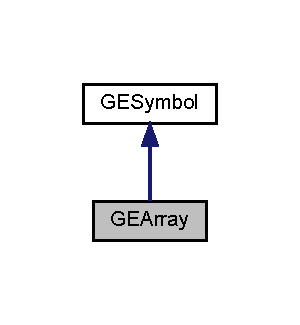
\includegraphics[width=144pt]{class_g_e_array__inherit__graph}
\end{center}
\end{figure}
\subsection*{Public Member Functions}
\begin{DoxyCompactItemize}
\item 
\hypertarget{class_g_e_array_a59934816e881cf01fb22d08f1d8fc1e0}{\hyperlink{class_g_e_array_a59934816e881cf01fb22d08f1d8fc1e0}{G\-E\-Array} ()}\label{class_g_e_array_a59934816e881cf01fb22d08f1d8fc1e0}

\begin{DoxyCompactList}\small\item\em Initialize a one dimensional array with a single element set to zero. \end{DoxyCompactList}\item 
\hyperlink{class_g_e_array_a99e59c84b9ee6288030cda2fecc116af}{G\-E\-Array} (vector$<$ int $>$ orders, V\-E\-C\-T\-O\-R\-\_\-\-D\-A\-T\-A(double) data, bool complex=false)
\begin{DoxyCompactList}\small\item\em Initialize an array with the orders specified. \end{DoxyCompactList}\item 
\hypertarget{class_g_e_array_aff83dc2b4d74f050eff84e360a8df3c9}{{\bfseries G\-E\-Array} (const int $\ast$orders, int orders\-\_\-len, const double $\ast$data, int data\-\_\-len, bool complex=false)}\label{class_g_e_array_aff83dc2b4d74f050eff84e360a8df3c9}

\item 
\hyperlink{class_g_e_matrix}{G\-E\-Matrix} $\ast$ \hyperlink{class_g_e_array_a760dc4efc92eb480a6892fe0336a5c13}{get\-Plane} (vector$<$ int $>$ orders, bool imag=false) const 
\begin{DoxyCompactList}\small\item\em Retrieve a 2-\/dimensional slice from an array. \end{DoxyCompactList}\item 
vector$<$ double $>$ \hyperlink{class_g_e_array_a157c2c5a9a96ba4d70873a502439c142}{get\-Vector} (vector$<$ int $>$ orders, bool imag=false) const 
\begin{DoxyCompactList}\small\item\em Retrieve a one dimensional vector from an array. \end{DoxyCompactList}\item 
double \hyperlink{class_g_e_array_a3eb9ae37593f93cd912242e34d864a7b}{get\-Element} (vector$<$ int $>$ orders, bool imag=false) const 
\begin{DoxyCompactList}\small\item\em Retrieve an element from an array. \end{DoxyCompactList}\item 
bool \hyperlink{class_g_e_array_a0e89787df523a69a1834c89adcfdfc3f}{set\-Element} (double, vector$<$ int $>$ orders, bool imag=false)
\begin{DoxyCompactList}\small\item\em Set an element in an array. \end{DoxyCompactList}\item 
vector$<$ double $>$ \hyperlink{class_g_e_array_a213163c7bc79ff072d3fe0de53afcdbe}{get\-Data} (bool imag=false) const 
\begin{DoxyCompactList}\small\item\em Retrieve a copy of underlying numeric vector. \end{DoxyCompactList}\item 
vector$<$ double $>$ \hyperlink{class_g_e_array_a88801ecb7d0845932a5df91e0d87f512}{get\-Imag\-Data} () const 
\begin{DoxyCompactList}\small\item\em Retrieve underlying imaginary data storage. \end{DoxyCompactList}\item 
vector$<$ int $>$ \hyperlink{class_g_e_array_aefb8352fe78692588d285be165267498}{get\-Orders} () const 
\begin{DoxyCompactList}\small\item\em Retrieve the vector of array orders. \end{DoxyCompactList}\item 
int \hyperlink{class_g_e_array_afad41971475ee5588ba8f5d0d396b5fc}{get\-Dimensions} () const 
\begin{DoxyCompactList}\small\item\em Return the number of array dimensions. \end{DoxyCompactList}\item 
virtual int \hyperlink{class_g_e_array_a4030556e997a324e09abcf46e6a9e7ef}{size} () const 
\begin{DoxyCompactList}\small\item\em Returns the total element count. \end{DoxyCompactList}\item 
virtual std\-::string \hyperlink{class_g_e_array_a9f0f5b80ff919ebbf663e0e2ad257512}{to\-String} () const 
\begin{DoxyCompactList}\small\item\em Returns a string representation of this object. \end{DoxyCompactList}\item 
virtual void \hyperlink{class_g_e_array_ad7fd6880da03d11c13387ea9e1e1cd5d}{clear} ()
\begin{DoxyCompactList}\small\item\em Clear all corresponding symbol data. \end{DoxyCompactList}\end{DoxyCompactItemize}
\subsection*{Friends}
\begin{DoxyCompactItemize}
\item 
\hypertarget{class_g_e_array_abc89e64d0ec6c939575c3125753c6309}{class {\bfseries G\-A\-U\-S\-S}}\label{class_g_e_array_abc89e64d0ec6c939575c3125753c6309}

\item 
\hypertarget{class_g_e_array_a2e5e14117f0e69078f45b8d512f056de}{class {\bfseries G\-A\-U\-S\-S\-Private}}\label{class_g_e_array_a2e5e14117f0e69078f45b8d512f056de}

\end{DoxyCompactItemize}
\subsection*{Additional Inherited Members}


\subsection{Detailed Description}
\hyperlink{class_g_a_u_s_s}{G\-A\-U\-S\-S} Array symbol type. 

This represents An N-\/dimensional array of double precision numbers. 

\subsection{Constructor \& Destructor Documentation}
\hypertarget{class_g_e_array_a99e59c84b9ee6288030cda2fecc116af}{\index{G\-E\-Array@{G\-E\-Array}!G\-E\-Array@{G\-E\-Array}}
\index{G\-E\-Array@{G\-E\-Array}!GEArray@{G\-E\-Array}}
\subsubsection[{G\-E\-Array}]{\setlength{\rightskip}{0pt plus 5cm}G\-E\-Array\-::\-G\-E\-Array (
\begin{DoxyParamCaption}
\item[{vector$<$ int $>$}]{orders, }
\item[{V\-E\-C\-T\-O\-R\-\_\-\-D\-A\-T\-A(double)}]{data, }
\item[{bool}]{complex = {\ttfamily false}}
\end{DoxyParamCaption}
)}}\label{class_g_e_array_a99e59c84b9ee6288030cda2fecc116af}


Initialize an array with the orders specified. 

You need to fill in the array data from lowest dimension to highest dimension. If the data is complex, it should contain all the real values in the first half of the array, followed by all the imaginary values in the second half of the array.

Example\-:

\subparagraph*{Python}


\begin{DoxyCode}
1 orders = [4, 3, 2]
2 data = range(1, 49)
3 a = \hyperlink{class_g_e_array}{GEArray}(orders, data, \textcolor{keyword}{True})     \textcolor{comment}{# Indicate data is complex}
\end{DoxyCode}


\subparagraph*{P\-H\-P}


\begin{DoxyCode}
$orders = array(4, 3, 2);
$data = range(1.0, 48.0);
$a = \textcolor{keyword}{new} \hyperlink{class_g_e_array_a59934816e881cf01fb22d08f1d8fc1e0}{GEArray}($orders, $data, \textcolor{keyword}{true}); \textcolor{comment}{// Indicate data is complex}
\end{DoxyCode}


will create a complex array with the elements filled in as follows\-:


\begin{DoxyCode}
[1,1,1] =  1.0 + 25.0i,  [1,1,2] =  2.0 + 26.0i,
[1,2,1] =  3.0 + 27.0i,  [1,2,2] =  4.0 + 28.0i,
[1,3,1] =  5.0 + 29.0i,  [1,3,2] =  6.0 + 30.0i,

[2,1,1] =  7.0 + 31.0i,  [2,1,2] =  8.0 + 32.0i,
[2,2,1] =  9.0 + 33.0i,  [2,2,2] = 10.0 + 34.0i,
[2,3,1] = 11.0 + 35.0i,  [2,3,2] = 12.0 + 36.0i,

...
\end{DoxyCode}



\begin{DoxyParams}{Parameters}
{\em orders} & Dimension orders from highest to lowest left-\/to-\/right. \\
\hline
{\em data} & Data in one dimensional format \\
\hline
{\em complex} & True if array is complex, false otherwise. \\
\hline
\end{DoxyParams}


\subsection{Member Function Documentation}
\hypertarget{class_g_e_array_ad7fd6880da03d11c13387ea9e1e1cd5d}{\index{G\-E\-Array@{G\-E\-Array}!clear@{clear}}
\index{clear@{clear}!GEArray@{G\-E\-Array}}
\subsubsection[{clear}]{\setlength{\rightskip}{0pt plus 5cm}void G\-E\-Array\-::clear (
\begin{DoxyParamCaption}
{}
\end{DoxyParamCaption}
)\hspace{0.3cm}{\ttfamily [virtual]}}}\label{class_g_e_array_ad7fd6880da03d11c13387ea9e1e1cd5d}


Clear all corresponding symbol data. 

Does not clear from workspace. 

Reimplemented from \hyperlink{class_g_e_symbol_a39d2e523aec771a73e1cc5d7a9618b88}{G\-E\-Symbol}.

\hypertarget{class_g_e_array_a213163c7bc79ff072d3fe0de53afcdbe}{\index{G\-E\-Array@{G\-E\-Array}!get\-Data@{get\-Data}}
\index{get\-Data@{get\-Data}!GEArray@{G\-E\-Array}}
\subsubsection[{get\-Data}]{\setlength{\rightskip}{0pt plus 5cm}vector$<$ double $>$ G\-E\-Array\-::get\-Data (
\begin{DoxyParamCaption}
\item[{bool}]{imag = {\ttfamily false}}
\end{DoxyParamCaption}
) const}}\label{class_g_e_array_a213163c7bc79ff072d3fe0de53afcdbe}


Retrieve a copy of underlying numeric vector. 

Imaginary data can also be queried by supplying the {\itshape imag} argument, thus appending it to the end of the real data. Omitting or specifying the {\itshape imag} argument as {\ttfamily false} will return only real data. If you wish to only view the imaginary data, there is a \hyperlink{class_g_e_array_a88801ecb7d0845932a5df91e0d87f512}{get\-Imag\-Data()} method for convenience.

Example\-:

\subparagraph*{Python}


\begin{DoxyCode}
1 \textcolor{comment}{# Create a 2x3x4 array with values 1.0 - 24.0}
2 ge.executeString(\textcolor{stringliteral}{"a = areshape(seqa(1, 1, 24), 2|3|4)"})
3 a = ge.getArray(\textcolor{stringliteral}{"a"})
4 \textcolor{keywordflow}{print} \textcolor{stringliteral}{", "}.join(str(n) \textcolor{keywordflow}{for} n \textcolor{keywordflow}{in} a.getData())
\end{DoxyCode}


\subparagraph*{P\-H\-P}


\begin{DoxyCode}
\textcolor{comment}{// Create a 2x3x4 array with values 1.0 - 24.0}
$ge->executeString(\textcolor{stringliteral}{"a = areshape(seqa(1, 1, 24), 2|3|4);"});
$a = $ge->getArray(\textcolor{stringliteral}{"a"});
echo implode(\textcolor{stringliteral}{", "}, $a->getData()) . PHP\_EOL;
\end{DoxyCode}
 will result in the output\-: 
\begin{DoxyCode}
1, 2, 3, 4, 5, 6, 7, 8, 9, 10, 11, 12, 13, 14, 15, 16, 17, 18, 19, 20, 21, 22, 23, 24
\end{DoxyCode}



\begin{DoxyParams}{Parameters}
{\em imag} & Whether to append imaginary data to end of real data \\
\hline
\end{DoxyParams}
\begin{DoxyReturn}{Returns}
Array data as a one-\/dimensional vector 
\end{DoxyReturn}
\hypertarget{class_g_e_array_afad41971475ee5588ba8f5d0d396b5fc}{\index{G\-E\-Array@{G\-E\-Array}!get\-Dimensions@{get\-Dimensions}}
\index{get\-Dimensions@{get\-Dimensions}!GEArray@{G\-E\-Array}}
\subsubsection[{get\-Dimensions}]{\setlength{\rightskip}{0pt plus 5cm}int G\-E\-Array\-::get\-Dimensions (
\begin{DoxyParamCaption}
{}
\end{DoxyParamCaption}
) const}}\label{class_g_e_array_afad41971475ee5588ba8f5d0d396b5fc}


Return the number of array dimensions. 

This should be equal to the length of \hyperlink{class_g_e_array_aefb8352fe78692588d285be165267498}{get\-Orders()}

Example\-:

\subparagraph*{Python}


\begin{DoxyCode}
1 \textcolor{comment}{# Create a 2x3x4 array with values 1.0 - 24.0}
2 ge.executeString(\textcolor{stringliteral}{"a = areshape(seqa(1, 1, 24), 2|3|4)"})
3 a = ge.getArray(\textcolor{stringliteral}{"a"})
4 \textcolor{keywordflow}{print} \textcolor{stringliteral}{"a dimensions = "} + str(a.getDimensions())
5 \textcolor{keywordflow}{print} \textcolor{stringliteral}{"a order count = "} + str(len(a.getOrders()))
\end{DoxyCode}


\subparagraph*{P\-H\-P}


\begin{DoxyCode}
\textcolor{comment}{// Create a 2x3x4 array with values 1.0 - 24.0}
$ge->executeString(\textcolor{stringliteral}{"a = areshape(seqa(1, 1, 24), 2|3|4);"});
$a = $ge->getArray(\textcolor{stringliteral}{"a"});
echo \textcolor{stringliteral}{"a dimensions = "} . $a->getDimensions() . PHP\_EOL;
echo \textcolor{stringliteral}{"a order count = "} . count($a->getOrders()) . PHP\_EOL
\end{DoxyCode}
 will result in the output\-: 
\begin{DoxyCode}
a dimensions = 3
a order count = 3
\end{DoxyCode}


\begin{DoxyReturn}{Returns}
Array dimension count 
\end{DoxyReturn}
\hypertarget{class_g_e_array_a3eb9ae37593f93cd912242e34d864a7b}{\index{G\-E\-Array@{G\-E\-Array}!get\-Element@{get\-Element}}
\index{get\-Element@{get\-Element}!GEArray@{G\-E\-Array}}
\subsubsection[{get\-Element}]{\setlength{\rightskip}{0pt plus 5cm}double G\-E\-Array\-::get\-Element (
\begin{DoxyParamCaption}
\item[{vector$<$ int $>$}]{indices, }
\item[{bool}]{imag = {\ttfamily false}}
\end{DoxyParamCaption}
) const}}\label{class_g_e_array_a3eb9ae37593f93cd912242e34d864a7b}


Retrieve an element from an array. 

The indices array will contain N normal indices into the array, indicating the element you want. This function only returns either the real or the imaginary part of the data based on the {\itshape imag} argument

Example\-:

\subparagraph*{Python}


\begin{DoxyCode}
1 \textcolor{comment}{# Create a 2x3x4 array with values 1.0 - 24.0}
2 ge.executeString(\textcolor{stringliteral}{"a = areshape(seqa(1, 1, 24), 2|3|4)"})
3 a = ge.getArray(\textcolor{stringliteral}{"a"})
4 \textcolor{keywordflow}{print} str(a.getElement([1, 1, 2])) \textcolor{comment}{# Second element on first row of first plane}
5 \textcolor{keywordflow}{print} str(a.getElement([1, 2, 1])) \textcolor{comment}{# First element on second row of first plane}
6 \textcolor{keywordflow}{print} str(a.getElement([2, 1, 1])) \textcolor{comment}{# First element on first row of second plane}
\end{DoxyCode}


\subparagraph*{P\-H\-P}


\begin{DoxyCode}
\textcolor{comment}{// Create a 2x3x4 array with values 1.0 - 24.0}
$ge->executeString(\textcolor{stringliteral}{"a = areshape(seqa(1, 1, 24), 2|3|4);"});
$a = $ge->getArray(\textcolor{stringliteral}{"a"});
echo $a->getElement(array(1, 1, 2)) . PHP\_EOL; \textcolor{comment}{// Second element on first row of first plane}
echo $a->getElement(array(1, 2, 1)) . PHP\_EOL; \textcolor{comment}{// First element on second row of first plane}
echo $a->getElement(array(2, 1, 1)) . PHP\_EOL; \textcolor{comment}{// First element on first row of second plane}
\end{DoxyCode}
 will result in the output\-: 
\begin{DoxyCode}
2
5
13
\end{DoxyCode}
 extracted from the values of a\-: 
\begin{DoxyCode}
Plane [1,.,.]

       1.0000000        2.0000000        3.0000000        4.0000000
       5.0000000        6.0000000        7.0000000        8.0000000
       9.0000000        10.000000        11.000000        12.000000

Plane [2,.,.]

       13.000000        14.000000        15.000000        16.000000
       17.000000        18.000000        19.000000        20.000000
       21.000000        22.000000        23.000000        24.000000
\end{DoxyCode}



\begin{DoxyParams}{Parameters}
{\em indices} & Indices indicating the element to retrieve \\
\hline
{\em imag} & Whether to return imaginary data instead of real data. \\
\hline
\end{DoxyParams}
\begin{DoxyReturn}{Returns}
double precision element 
\end{DoxyReturn}
\hypertarget{class_g_e_array_a88801ecb7d0845932a5df91e0d87f512}{\index{G\-E\-Array@{G\-E\-Array}!get\-Imag\-Data@{get\-Imag\-Data}}
\index{get\-Imag\-Data@{get\-Imag\-Data}!GEArray@{G\-E\-Array}}
\subsubsection[{get\-Imag\-Data}]{\setlength{\rightskip}{0pt plus 5cm}vector$<$ double $>$ G\-E\-Array\-::get\-Imag\-Data (
\begin{DoxyParamCaption}
{}
\end{DoxyParamCaption}
) const}}\label{class_g_e_array_a88801ecb7d0845932a5df91e0d87f512}


Retrieve underlying imaginary data storage. 

This will be stored in lowest to highest dimension.

Example\-:

\subparagraph*{Python}


\begin{DoxyCode}
1 \textcolor{comment}{# Create a 2x3x4 array with values 1.0 - 24.0}
2 ge.executeString(\textcolor{stringliteral}{"a = areshape(seqa(1, 1, 24), 2|3|4)"})
3 ge.executeString(\textcolor{stringliteral}{"b = areshape(seqa(25, 1, 24), 2|3|4)"})
4 ge.executeString(\textcolor{stringliteral}{"c = complex(a, b)"})
5 c = ge.getArray(\textcolor{stringliteral}{"c"})
6 \textcolor{keywordflow}{print} \textcolor{stringliteral}{", "}.join(str(n) \textcolor{keywordflow}{for} n \textcolor{keywordflow}{in} c.getImagData())
\end{DoxyCode}


\subparagraph*{P\-H\-P}


\begin{DoxyCode}
\textcolor{comment}{// Create a 2x3x4 array with values 1.0 - 24.0}
$ge->executeString(\textcolor{stringliteral}{"a = areshape(seqa(1, 1, 24), 2|3|4)"});
$ge->executeString(\textcolor{stringliteral}{"b = areshape(seqa(25, 1, 24), 2|3|4)"});
$ge->executeString(\textcolor{stringliteral}{"c = complex(a, b)"});
$c = $ge->getArray(\textcolor{stringliteral}{"c"});
echo implode(\textcolor{stringliteral}{", "}, $c->getImagData()) . PHP\_EOL;
\end{DoxyCode}
 will result in the output\-: 
\begin{DoxyCode}
25.0, 26.0, 27.0, 28.0, 29.0, 30.0, 31.0, 32.0, 33.0, 34.0, 35.0, 36.0, 37.0, 38.0, 39.0, 40.0, 41.0, 42.0,
       43.0, 44.0, 45.0, 46.0, 47.0, 48.0
\end{DoxyCode}


\begin{DoxyReturn}{Returns}
Array data as a one-\/dimensional vector 
\end{DoxyReturn}
\hypertarget{class_g_e_array_aefb8352fe78692588d285be165267498}{\index{G\-E\-Array@{G\-E\-Array}!get\-Orders@{get\-Orders}}
\index{get\-Orders@{get\-Orders}!GEArray@{G\-E\-Array}}
\subsubsection[{get\-Orders}]{\setlength{\rightskip}{0pt plus 5cm}vector$<$ int $>$ G\-E\-Array\-::get\-Orders (
\begin{DoxyParamCaption}
{}
\end{DoxyParamCaption}
) const}}\label{class_g_e_array_aefb8352fe78692588d285be165267498}


Retrieve the vector of array orders. 

These are ordered from highest to lowest.

Example\-:

\subparagraph*{Python}


\begin{DoxyCode}
1 \textcolor{comment}{# Create a 2x3x4 array with values 1.0 - 24.0}
2 ge.executeString(\textcolor{stringliteral}{"a = areshape(seqa(1, 1, 24), 2|3|4)"})
3 a = ge.getArray(\textcolor{stringliteral}{"a"})
4 \textcolor{keywordflow}{print} \textcolor{stringliteral}{"a orders = "} + \textcolor{stringliteral}{"x"}.join(str(n) \textcolor{keywordflow}{for} n \textcolor{keywordflow}{in} a.getOrders())
\end{DoxyCode}


\subparagraph*{P\-H\-P}


\begin{DoxyCode}
\textcolor{comment}{// Create a 2x3x4 array with values 1.0 - 24.0}
$ge->executeString(\textcolor{stringliteral}{"a = areshape(seqa(1, 1, 24), 2|3|4);"});
$a = $ge->getArray(\textcolor{stringliteral}{"a"});
echo \textcolor{stringliteral}{"a orders = "} . implode(\textcolor{stringliteral}{"x"}, $a->getOrders()) . PHP\_EOL;
\end{DoxyCode}
 will result in the output\-: 
\begin{DoxyCode}
a orders = 2x3x4
\end{DoxyCode}


\begin{DoxyReturn}{Returns}
Vector of array orders 
\end{DoxyReturn}
\hypertarget{class_g_e_array_a760dc4efc92eb480a6892fe0336a5c13}{\index{G\-E\-Array@{G\-E\-Array}!get\-Plane@{get\-Plane}}
\index{get\-Plane@{get\-Plane}!GEArray@{G\-E\-Array}}
\subsubsection[{get\-Plane}]{\setlength{\rightskip}{0pt plus 5cm}{\bf G\-E\-Matrix} $\ast$ G\-E\-Array\-::get\-Plane (
\begin{DoxyParamCaption}
\item[{vector$<$ int $>$}]{indices, }
\item[{bool}]{imag = {\ttfamily false}}
\end{DoxyParamCaption}
) const}}\label{class_g_e_array_a760dc4efc92eb480a6892fe0336a5c13}


Retrieve a 2-\/dimensional slice from an array. 

The indices array will contain N-\/2 normal indices into the array, positioning to the first element of the plane of interest, and two indices set to 0, indicating the dimensions of interest. The plane of elements across those 2 dimensions will be returned, the lower dimension becoming columns and the higher dimension becoming rows. This function returns either the real or the imaginary part of the data, based on the {\itshape imag} argument.

If you need to extract more than two dimensions of data, you can use the \hyperlink{class_g_a_u_s_s}{G\-A\-U\-S\-S} indexing (square bracket) operators or the G\-A\-U\-S\-S.\-get\-Array(string) function. See the N-\/\-Dimensional Arrays and Working With Arrays chapters of the \hyperlink{class_g_a_u_s_s}{G\-A\-U\-S\-S} User Guide.

Example\-:

\subparagraph*{Python}


\begin{DoxyCode}
1 ge.executeString(\textcolor{stringliteral}{"a = areshape(seqa(1, 1, 24), 2|3|4)"})
2 a = ge.getArray(\textcolor{stringliteral}{"a"})
3 
4 \textcolor{comment}{# p is now a GEMatrix object}
5 p = a.getPlane([0, 2, 0])
6 
7 \textcolor{keywordflow}{for} i \textcolor{keywordflow}{in} range(0, p.getRows()):
8     \textcolor{keywordflow}{for} j \textcolor{keywordflow}{in} range(0, p.getCols()):
9         \textcolor{keywordflow}{print} str(p.getElement(i, j)) + \textcolor{stringliteral}{"\(\backslash\)t"},
10 
11     \textcolor{keywordflow}{print}
\end{DoxyCode}


\subparagraph*{P\-H\-P}


\begin{DoxyCode}
$ge->executeString(\textcolor{stringliteral}{"a = areshape(seqa(1, 1, 24), 2|3|4);"});
$a = $ge->getArray(\textcolor{stringliteral}{"a"});

\textcolor{comment}{// $p is now a GEMatrix object}
$p = $a->getPlane(array(0, 2, 0));

\textcolor{keywordflow}{for} ($i = 0; $i < $p->getRows(); ++$i) \{
    \textcolor{keywordflow}{for} ($j = 0; $j < $p->getCols(); ++$j) \{
        echo $p->getElement($i, $j) . \textcolor{stringliteral}{"\(\backslash\)t"};
    \}

    echo PHP\_EOL;
\}
\end{DoxyCode}
 will result in the output\-: 
\begin{DoxyCode}
5        6        7        8
17        18        19        20
\end{DoxyCode}
 extracted from the values of a\-: 
\begin{DoxyCode}
Plane [1,.,.]

       1.0000000        2.0000000        3.0000000        4.0000000
       5.0000000        6.0000000        7.0000000        8.0000000
       9.0000000        10.000000        11.000000        12.000000

Plane [2,.,.]

       13.000000        14.000000        15.000000        16.000000
       17.000000        18.000000        19.000000        20.000000
       21.000000        22.000000        23.000000        24.000000
\end{DoxyCode}



\begin{DoxyParams}{Parameters}
{\em indices} & Indices indicating the plane to retrieve, with 0's representing the dimensions of interest \\
\hline
{\em imag} & Whether to return imaginary data instead of real data. \\
\hline
\end{DoxyParams}
\begin{DoxyReturn}{Returns}
2 dimensional array slice. 
\end{DoxyReturn}
\hypertarget{class_g_e_array_a157c2c5a9a96ba4d70873a502439c142}{\index{G\-E\-Array@{G\-E\-Array}!get\-Vector@{get\-Vector}}
\index{get\-Vector@{get\-Vector}!GEArray@{G\-E\-Array}}
\subsubsection[{get\-Vector}]{\setlength{\rightskip}{0pt plus 5cm}vector$<$ double $>$ G\-E\-Array\-::get\-Vector (
\begin{DoxyParamCaption}
\item[{vector$<$ int $>$}]{indices, }
\item[{bool}]{imag = {\ttfamily false}}
\end{DoxyParamCaption}
) const}}\label{class_g_e_array_a157c2c5a9a96ba4d70873a502439c142}


Retrieve a one dimensional vector from an array. 

The dimension of interest must be specified with a 0. This will get a vector of elements across the dimension. This function only returns either the real or the imaginary part of the data based on the {\itshape imag} argument.

Example\-:

\subparagraph*{Python}


\begin{DoxyCode}
1 ge.executeString(\textcolor{stringliteral}{"a = areshape(seqa(1, 1, 24), 2|3|4)"})
2 a = ge.getArray(\textcolor{stringliteral}{"a"})
3 
4 \textcolor{comment}{# p is now a GEMatrix object}
5 v = a.getVector([0, 3, 4])
6 
7 \textcolor{keywordflow}{print} \textcolor{stringliteral}{", "}.join([str(n) \textcolor{keywordflow}{for} n \textcolor{keywordflow}{in} v])
\end{DoxyCode}


\subparagraph*{P\-H\-P}


\begin{DoxyCode}
$ge->executeString(\textcolor{stringliteral}{"a = areshape(seqa(1, 1, 24), 2|3|4);"});
$a = $ge->getArray(\textcolor{stringliteral}{"a"});

\textcolor{comment}{// $p is now a GEMatrix object}
$v = $a->getVector(array(0, 3, 4));

echo implode(\textcolor{stringliteral}{", "}, $v) . PHP\_EOL;
\end{DoxyCode}
 will result in the output\-: 
\begin{DoxyCode}
12, 24
\end{DoxyCode}
 extracted from the value of a\-: 
\begin{DoxyCode}
Plane [1,.,.]

       1.0000000        2.0000000        3.0000000        4.0000000
       5.0000000        6.0000000        7.0000000        8.0000000
       9.0000000        10.000000        11.000000        12.000000

Plane [2,.,.]

       13.000000        14.000000        15.000000        16.000000
       17.000000        18.000000        19.000000        20.000000
       21.000000        22.000000        23.000000        24.000000
\end{DoxyCode}



\begin{DoxyParams}{Parameters}
{\em indices} & Indices that you would like to retrieve, with a 0 representing the dimension of interest \\
\hline
{\em imag} & Whether to return imaginary data instead of real data. \\
\hline
\end{DoxyParams}
\begin{DoxyReturn}{Returns}
Vector of data 
\end{DoxyReturn}
\hypertarget{class_g_e_array_a0e89787df523a69a1834c89adcfdfc3f}{\index{G\-E\-Array@{G\-E\-Array}!set\-Element@{set\-Element}}
\index{set\-Element@{set\-Element}!GEArray@{G\-E\-Array}}
\subsubsection[{set\-Element}]{\setlength{\rightskip}{0pt plus 5cm}bool G\-E\-Array\-::set\-Element (
\begin{DoxyParamCaption}
\item[{double}]{value, }
\item[{vector$<$ int $>$}]{indices, }
\item[{bool}]{imag = {\ttfamily false}}
\end{DoxyParamCaption}
)}}\label{class_g_e_array_a0e89787df523a69a1834c89adcfdfc3f}


Set an element in an array. 

The indices array will contain N normal indices into the array, indicating the element you want to set the new value of. This function sets either the real or the imaginary part of the data based on the {\itshape imag} argument.

Example\-:

\subparagraph*{Python}


\begin{DoxyCode}
1 \textcolor{comment}{# Create a 2x3x4 array with values 1.0 - 24.0}
2 ge.executeString(\textcolor{stringliteral}{"a = areshape(seqa(1, 1, 24), 2|3|4)"})
3 a = ge.getArray(\textcolor{stringliteral}{"a"})
4 a.setElement(0, [1, 1, 2]) \textcolor{comment}{# Second element on first row of first plane}
5 a.setElement(0, [1, 2, 1]) \textcolor{comment}{# First element on second row of first plane}
6 a.setElement(0, [2, 1, 1]) \textcolor{comment}{# First element on first row of second plane}
7 ge.setSymbol(a, \textcolor{stringliteral}{"a"})
8 ge.executeString(\textcolor{stringliteral}{"print a"})
\end{DoxyCode}


\subparagraph*{P\-H\-P}


\begin{DoxyCode}
\textcolor{comment}{// Create a 2x3x4 array with values 1.0 - 24.0}
$ge->executeString(\textcolor{stringliteral}{"a = areshape(seqa(1, 1, 24), 2|3|4);"});
$a = $ge->getArray(\textcolor{stringliteral}{"a"});
$a->setElement(0, array(1, 1, 2)); \textcolor{comment}{// Second element on first row of first plane}
$a->setElement(0, array(1, 2, 1)); \textcolor{comment}{// First element on second row of first plane}
$a->setElement(0, array(2, 1, 1)); \textcolor{comment}{// First element on first row of second plane}
$ge->setSymbol($a, \textcolor{stringliteral}{"a"});
$ge->executeString(\textcolor{stringliteral}{"print a;"});
\end{DoxyCode}
 will result in the output\-: 
\begin{DoxyCode}
Plane [1,.,.]

       1.0000000        0.0000000        3.0000000        4.0000000
       0.0000000        6.0000000        7.0000000        8.0000000
       9.0000000        10.000000        11.000000        12.000000

Plane [2,.,.]

        0.000000        14.000000        15.000000        16.000000
       17.000000        18.000000        19.000000        20.000000
       21.000000        22.000000        23.000000        24.000000
\end{DoxyCode}
 extracted from the values of a\-: 
\begin{DoxyCode}
Plane [1,.,.]

       1.0000000        2.0000000        3.0000000        4.0000000
       5.0000000        6.0000000        7.0000000        8.0000000
       9.0000000        10.000000        11.000000        12.000000

Plane [2,.,.]

       13.000000        14.000000        15.000000        16.000000
       17.000000        18.000000        19.000000        20.000000
       21.000000        22.000000        23.000000        24.000000
\end{DoxyCode}



\begin{DoxyParams}{Parameters}
{\em value} & Double precision value to set at element index \\
\hline
{\em indices} & Indices indicating the element to set \\
\hline
{\em imag} & Whether to set imaginary data instead of real data. \\
\hline
\end{DoxyParams}
\hypertarget{class_g_e_array_a4030556e997a324e09abcf46e6a9e7ef}{\index{G\-E\-Array@{G\-E\-Array}!size@{size}}
\index{size@{size}!GEArray@{G\-E\-Array}}
\subsubsection[{size}]{\setlength{\rightskip}{0pt plus 5cm}int G\-E\-Array\-::size (
\begin{DoxyParamCaption}
{}
\end{DoxyParamCaption}
) const\hspace{0.3cm}{\ttfamily [virtual]}}}\label{class_g_e_array_a4030556e997a324e09abcf46e6a9e7ef}


Returns the total element count. 

This is the product of \hyperlink{class_g_e_array_aefb8352fe78692588d285be165267498}{get\-Orders()}.

\begin{DoxyReturn}{Returns}
Total element count 
\end{DoxyReturn}


Reimplemented from \hyperlink{class_g_e_symbol_a9dfb28fc5c1a67658c5380d5fbdfbc24}{G\-E\-Symbol}.

\hypertarget{class_g_e_array_a9f0f5b80ff919ebbf663e0e2ad257512}{\index{G\-E\-Array@{G\-E\-Array}!to\-String@{to\-String}}
\index{to\-String@{to\-String}!GEArray@{G\-E\-Array}}
\subsubsection[{to\-String}]{\setlength{\rightskip}{0pt plus 5cm}string G\-E\-Array\-::to\-String (
\begin{DoxyParamCaption}
{}
\end{DoxyParamCaption}
) const\hspace{0.3cm}{\ttfamily [virtual]}}}\label{class_g_e_array_a9f0f5b80ff919ebbf663e0e2ad257512}


Returns a string representation of this object. 



Reimplemented from \hyperlink{class_g_e_symbol_ac79ba555226072d4b03f06e9f8bb6afb}{G\-E\-Symbol}.



The documentation for this class was generated from the following files\-:\begin{DoxyCompactItemize}
\item 
src/gearray.\-h\item 
src/gearray.\-cpp\end{DoxyCompactItemize}

\hypertarget{class_g_e_matrix}{\section{G\-E\-Matrix Class Reference}
\label{class_g_e_matrix}\index{G\-E\-Matrix@{G\-E\-Matrix}}
}


\hyperlink{class_g_a_u_s_s}{G\-A\-U\-S\-S} Matrix symbol type.  




{\ttfamily \#include $<$gematrix.\-h$>$}



Inheritance diagram for G\-E\-Matrix\-:
\nopagebreak
\begin{figure}[H]
\begin{center}
\leavevmode
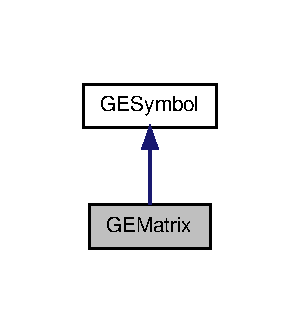
\includegraphics[width=144pt]{class_g_e_matrix__inherit__graph}
\end{center}
\end{figure}
\subsection*{Public Member Functions}
\begin{DoxyCompactItemize}
\item 
\hyperlink{class_g_e_matrix_a8efdf9ec85fdcfa0e9f1317722e81c52}{G\-E\-Matrix} ()
\begin{DoxyCompactList}\small\item\em Construct a {\ttfamily 1x1} matrix with value of {\ttfamily 0}. \end{DoxyCompactList}\item 
\hyperlink{class_g_e_matrix_af9ebcc214a2086c4692fa107c3ee53e9}{G\-E\-Matrix} (double)
\begin{DoxyCompactList}\small\item\em Initialize matrix to scalar with specified value. \end{DoxyCompactList}\item 
\hyperlink{class_g_e_matrix_ac48ac546516c7fb55a601f3875a5b23d}{G\-E\-Matrix} (vector$<$ double $>$)
\begin{DoxyCompactList}\small\item\em Construct a matrix object from a vector of double-\/precision numbers with {\ttfamily data.\-size()} columns and 1 row. \end{DoxyCompactList}\item 
\hyperlink{class_g_e_matrix_a926e3559025f6670e228b1c845457faa}{G\-E\-Matrix} (vector$<$ double $>$, int rows, int cols, bool complex=false)
\begin{DoxyCompactList}\small\item\em Construct a real matrix with {\itshape rows} rows, and {\itshape cols} columns. \end{DoxyCompactList}\item 
\hyperlink{class_g_e_matrix_aca44eb90745693a11023911071aee70a}{G\-E\-Matrix} (vector$<$ double $>$, vector$<$ double $>$, int rows, int cols)
\begin{DoxyCompactList}\small\item\em Construct a complex matrix. \end{DoxyCompactList}\item 
bool \hyperlink{class_g_e_matrix_a598ff86c462efb947271a067929f9c92}{set\-Element} (double, bool imag=false)
\begin{DoxyCompactList}\small\item\em Set the first value in matrix. \end{DoxyCompactList}\item 
bool \hyperlink{class_g_e_matrix_a0f9910054bf5faf4074784a5ce1ba4bb}{set\-Element} (double, int row, int col, bool imag=false)
\begin{DoxyCompactList}\small\item\em Set a value in the matrix at the specified row/column index. \end{DoxyCompactList}\item 
double \hyperlink{class_g_e_matrix_a37be9c3ae20e6adc9968e0770d71d42d}{get\-Element} (bool imag=false)
\begin{DoxyCompactList}\small\item\em Returns the first value from a matrix. \end{DoxyCompactList}\item 
double \hyperlink{class_g_e_matrix_ae74f09cd9e8dd209301646de6fc34766}{get\-Element} (int row, int col, bool imag=false)
\begin{DoxyCompactList}\small\item\em Returns a value from the matrix at the specified row/column index. \end{DoxyCompactList}\item 
vector$<$ double $>$ \hyperlink{class_g_e_matrix_af5e9d6f29599ab9344d4f7e163dd7d61}{get\-Data} (bool imag=false)
\begin{DoxyCompactList}\small\item\em Retrieve a copy of underlying numeric vector. \end{DoxyCompactList}\item 
vector$<$ double $>$ \hyperlink{class_g_e_matrix_a5bcef5af3933e59df30bfbc40d0d53ee}{get\-Imag\-Data} ()
\begin{DoxyCompactList}\small\item\em Retrieve a copy of underlying imaginary data storage. \end{DoxyCompactList}\item 
virtual void \hyperlink{class_g_e_matrix_a1bf6ddd9f46248e1c03c0d952d572103}{clear} ()
\begin{DoxyCompactList}\small\item\em Clear all corresponding symbol data. \end{DoxyCompactList}\item 
virtual std\-::string \hyperlink{class_g_e_matrix_a6f46cc050d3f8966a01676791b362387}{to\-String} ()
\begin{DoxyCompactList}\small\item\em Returns a string representation of this object. \end{DoxyCompactList}\end{DoxyCompactItemize}
\subsection*{Friends}
\begin{DoxyCompactItemize}
\item 
\hypertarget{class_g_e_matrix_abc89e64d0ec6c939575c3125753c6309}{class {\bfseries G\-A\-U\-S\-S}}\label{class_g_e_matrix_abc89e64d0ec6c939575c3125753c6309}

\end{DoxyCompactItemize}
\subsection*{Additional Inherited Members}


\subsection{Detailed Description}
\hyperlink{class_g_a_u_s_s}{G\-A\-U\-S\-S} Matrix symbol type. 

Represents two dimensional array of double precision numbers. Matrices can also be complex, storing both real and imaginary data. 

\subsection{Constructor \& Destructor Documentation}
\hypertarget{class_g_e_matrix_a8efdf9ec85fdcfa0e9f1317722e81c52}{\index{G\-E\-Matrix@{G\-E\-Matrix}!G\-E\-Matrix@{G\-E\-Matrix}}
\index{G\-E\-Matrix@{G\-E\-Matrix}!GEMatrix@{G\-E\-Matrix}}
\subsubsection[{G\-E\-Matrix}]{\setlength{\rightskip}{0pt plus 5cm}G\-E\-Matrix\-::\-G\-E\-Matrix (
\begin{DoxyParamCaption}
{}
\end{DoxyParamCaption}
)}}\label{class_g_e_matrix_a8efdf9ec85fdcfa0e9f1317722e81c52}


Construct a {\ttfamily 1x1} matrix with value of {\ttfamily 0}. 

Example\-:

\subparagraph*{Python}


\begin{DoxyCode}
1 x = \hyperlink{class_g_e_matrix}{GEMatrix}()
2 ge.setSymbol(x, \textcolor{stringliteral}{"x"})
3 ge.executeString(\textcolor{stringliteral}{"print x"})
\end{DoxyCode}


\subparagraph*{P\-H\-P}


\begin{DoxyCode}
$x = \textcolor{keyword}{new} \hyperlink{class_g_e_matrix_a8efdf9ec85fdcfa0e9f1317722e81c52}{GEMatrix}();
$ge->setSymbol($x, \textcolor{stringliteral}{"x"});
$ge->executeString(\textcolor{stringliteral}{"print x;"});
\end{DoxyCode}
 results in output\-: 
\begin{DoxyCode}
0.0000000
\end{DoxyCode}
 \hypertarget{class_g_e_matrix_af9ebcc214a2086c4692fa107c3ee53e9}{\index{G\-E\-Matrix@{G\-E\-Matrix}!G\-E\-Matrix@{G\-E\-Matrix}}
\index{G\-E\-Matrix@{G\-E\-Matrix}!GEMatrix@{G\-E\-Matrix}}
\subsubsection[{G\-E\-Matrix}]{\setlength{\rightskip}{0pt plus 5cm}G\-E\-Matrix\-::\-G\-E\-Matrix (
\begin{DoxyParamCaption}
\item[{double}]{n}
\end{DoxyParamCaption}
)}}\label{class_g_e_matrix_af9ebcc214a2086c4692fa107c3ee53e9}


Initialize matrix to scalar with specified value. 

Example\-:

\subparagraph*{Python}


\begin{DoxyCode}
1 x = \hyperlink{class_g_e_matrix}{GEMatrix}(1.0)
2 ge.setSymbol(x, \textcolor{stringliteral}{"x"})
3 ge.executeString(\textcolor{stringliteral}{"print x"})
\end{DoxyCode}


\subparagraph*{P\-H\-P}


\begin{DoxyCode}
$x = \textcolor{keyword}{new} \hyperlink{class_g_e_matrix_a8efdf9ec85fdcfa0e9f1317722e81c52}{GEMatrix}(1.0);
$ge->setSymbol($x, \textcolor{stringliteral}{"x"});
$ge->executeString(\textcolor{stringliteral}{"print x;"});
\end{DoxyCode}
 results in output\-: 
\begin{DoxyCode}
1.0000000
\end{DoxyCode}



\begin{DoxyParams}{Parameters}
{\em d} & Scalar value \\
\hline
\end{DoxyParams}
\hypertarget{class_g_e_matrix_ac48ac546516c7fb55a601f3875a5b23d}{\index{G\-E\-Matrix@{G\-E\-Matrix}!G\-E\-Matrix@{G\-E\-Matrix}}
\index{G\-E\-Matrix@{G\-E\-Matrix}!GEMatrix@{G\-E\-Matrix}}
\subsubsection[{G\-E\-Matrix}]{\setlength{\rightskip}{0pt plus 5cm}G\-E\-Matrix\-::\-G\-E\-Matrix (
\begin{DoxyParamCaption}
\item[{vector$<$ double $>$}]{data}
\end{DoxyParamCaption}
)}}\label{class_g_e_matrix_ac48ac546516c7fb55a601f3875a5b23d}


Construct a matrix object from a vector of double-\/precision numbers with {\ttfamily data.\-size()} columns and 1 row. 

Example\-:

\subparagraph*{Python}


\begin{DoxyCode}
1 x = \hyperlink{class_g_e_matrix}{GEMatrix}([1.0, 2.0, 3.0, 4.0, 5.0, 6.0, 7.0, 8.0])
2 ge.setSymbol(x, \textcolor{stringliteral}{"x"})
3 ge.executeString(\textcolor{stringliteral}{"print x"})
\end{DoxyCode}


\subparagraph*{P\-H\-P}


\begin{DoxyCode}
$x = \textcolor{keyword}{new} \hyperlink{class_g_e_matrix_a8efdf9ec85fdcfa0e9f1317722e81c52}{GEMatrix}(array(1.0, 2.0, 3.0, 4.0, 5.0, 6.0, 7.0, 8.0));
$ge->setSymbol($x, \textcolor{stringliteral}{"x"});
$ge->executeString(\textcolor{stringliteral}{"print x;"});
\end{DoxyCode}
 results in output\-: 
\begin{DoxyCode}
1.0000000        2.0000000        3.0000000        4.0000000        5.0000000        6.0000000        7.000
      0000        8.0000000
\end{DoxyCode}



\begin{DoxyParams}{Parameters}
{\em data} & Data vector\\
\hline
\end{DoxyParams}
\begin{DoxySeeAlso}{See Also}
\hyperlink{class_g_e_matrix_a926e3559025f6670e228b1c845457faa}{G\-E\-Matrix(vector$<$double$>$, int, int, bool)} 

\hyperlink{class_g_e_matrix_aca44eb90745693a11023911071aee70a}{G\-E\-Matrix(vector$<$double$>$, vector$<$double$>$, int, int)} 
\end{DoxySeeAlso}
\hypertarget{class_g_e_matrix_a926e3559025f6670e228b1c845457faa}{\index{G\-E\-Matrix@{G\-E\-Matrix}!G\-E\-Matrix@{G\-E\-Matrix}}
\index{G\-E\-Matrix@{G\-E\-Matrix}!GEMatrix@{G\-E\-Matrix}}
\subsubsection[{G\-E\-Matrix}]{\setlength{\rightskip}{0pt plus 5cm}G\-E\-Matrix\-::\-G\-E\-Matrix (
\begin{DoxyParamCaption}
\item[{vector$<$ double $>$}]{data, }
\item[{int}]{rows, }
\item[{int}]{cols, }
\item[{bool}]{complex = {\ttfamily false}}
\end{DoxyParamCaption}
)}}\label{class_g_e_matrix_a926e3559025f6670e228b1c845457faa}


Construct a real matrix with {\itshape rows} rows, and {\itshape cols} columns. 

If {\itshape complex} is set to {\bfseries true}, {\ttfamily data.\-length()} must be {\itshape rows} $\ast$ {\itshape cols} $\ast$ 2

Example\-:

\subparagraph*{Python}


\begin{DoxyCode}
1 \textcolor{comment}{# Create a matrix}
2 x = \hyperlink{class_g_e_matrix}{GEMatrix}([1.0, 2.0, 3.0, 4.0, 5.0, 6.0, 7.0, 8.0], 4, 2)
3 ge.setSymbol(x, \textcolor{stringliteral}{"x"})
4 ge.executeString(\textcolor{stringliteral}{"print x"})
5 
6 \textcolor{comment}{# Create a matrix with imaginary data}
7 xc = \hyperlink{class_g_e_matrix}{GEMatrix}([1.0, 2.0, 3.0, 4.0, 5.0, 6.0, 7.0, 8.0], 2, 2, \textcolor{keyword}{True})
8 ge.setSymbol(xc, \textcolor{stringliteral}{"xc"})
9 ge.executeString(\textcolor{stringliteral}{"print xc"})
\end{DoxyCode}


\subparagraph*{P\-H\-P}


\begin{DoxyCode}
\textcolor{comment}{// Create a matrix}
$x = \textcolor{keyword}{new} \hyperlink{class_g_e_matrix_a8efdf9ec85fdcfa0e9f1317722e81c52}{GEMatrix}(array(1.0, 2.0, 3.0, 4.0, 5.0, 6.0, 7.0, 8.0), 4, 2);
$ge->setSymbol($x, \textcolor{stringliteral}{"x"});
$ge->executeString(\textcolor{stringliteral}{"print x;"});

\textcolor{comment}{// Create a matrix with imaginary data}
$xc = \textcolor{keyword}{new} \hyperlink{class_g_e_matrix_a8efdf9ec85fdcfa0e9f1317722e81c52}{GEMatrix}(array(1.0, 2.0, 3.0, 4.0, 5.0, 6.0, 7.0, 8.0), 2, 2, \textcolor{keyword}{true});
$ge->setSymbol($xc, \textcolor{stringliteral}{"xc"});
$ge->executeString(\textcolor{stringliteral}{"print xc;"});
\end{DoxyCode}
 results in output\-: 
\begin{DoxyCode}
1.0000000        2.0000000
3.0000000        4.0000000
5.0000000        6.0000000
7.0000000        8.0000000

1.0000000 +        5.0000000i        2.0000000 +        6.0000000i
3.0000000 +        7.0000000i        4.0000000 +        8.0000000i
\end{DoxyCode}



\begin{DoxyParams}{Parameters}
{\em data} & Vector of double precision values \\
\hline
{\em rows} & Number of rows \\
\hline
{\em cols} & Number of columns \\
\hline
{\em complex} & True if including imaginary data, false otherwise\\
\hline
\end{DoxyParams}
\begin{DoxySeeAlso}{See Also}
\hyperlink{class_g_e_matrix_aca44eb90745693a11023911071aee70a}{G\-E\-Matrix(vector$<$double$>$, vector$<$double$>$, int, int)} 
\end{DoxySeeAlso}
\hypertarget{class_g_e_matrix_aca44eb90745693a11023911071aee70a}{\index{G\-E\-Matrix@{G\-E\-Matrix}!G\-E\-Matrix@{G\-E\-Matrix}}
\index{G\-E\-Matrix@{G\-E\-Matrix}!GEMatrix@{G\-E\-Matrix}}
\subsubsection[{G\-E\-Matrix}]{\setlength{\rightskip}{0pt plus 5cm}G\-E\-Matrix\-::\-G\-E\-Matrix (
\begin{DoxyParamCaption}
\item[{vector$<$ double $>$}]{real\-\_\-data, }
\item[{vector$<$ double $>$}]{imag\-\_\-data, }
\item[{int}]{rows, }
\item[{int}]{cols}
\end{DoxyParamCaption}
)}}\label{class_g_e_matrix_aca44eb90745693a11023911071aee70a}


Construct a complex matrix. 

Uses {\itshape real\-\_\-data} for real data and {\itshape imag\-\_\-data} for imaginary data, with {\itshape rows} rows, and {\itshape cols} columns.

Example\-:

\subparagraph*{Python}


\begin{DoxyCode}
1 \textcolor{comment}{# Create a matrix with imaginary data}
2 xc = \hyperlink{class_g_e_matrix}{GEMatrix}([1.0, 2.0, 3.0, 4.0], [5.0, 6.0, 7.0, 8.0], 2, 2)
3 ge.setSymbol(xc, \textcolor{stringliteral}{"xc"})
4 ge.executeString(\textcolor{stringliteral}{"print xc"})
\end{DoxyCode}


\subparagraph*{P\-H\-P}


\begin{DoxyCode}
\textcolor{comment}{// Create a matrix with imaginary data}
$xc = \textcolor{keyword}{new} \hyperlink{class_g_e_matrix_a8efdf9ec85fdcfa0e9f1317722e81c52}{GEMatrix}(array(1.0, 2.0, 3.0, 4.0), array(5.0, 6.0, 7.0, 8.0), 2, 2);
$ge->setSymbol($xc, \textcolor{stringliteral}{"xc"});
$ge->executeString(\textcolor{stringliteral}{"print xc;"});
\end{DoxyCode}
 results in output\-: 
\begin{DoxyCode}
1.0000000 +        5.0000000i        2.0000000 +        6.0000000i
3.0000000 +        7.0000000i        4.0000000 +        8.0000000i
\end{DoxyCode}



\begin{DoxyParams}{Parameters}
{\em real\-\_\-data} & Vector of real double precision values \\
\hline
{\em imag\-\_\-data} & Vector of imaginary double precision values \\
\hline
{\em rows} & Number of rows \\
\hline
{\em cols} & Number of columns \\
\hline
{\em complex} & True if including imaginary data, false otherwise\\
\hline
\end{DoxyParams}
\begin{DoxySeeAlso}{See Also}
\hyperlink{class_g_e_matrix_a926e3559025f6670e228b1c845457faa}{G\-E\-Matrix(vector$<$double$>$, int, int, bool)} 
\end{DoxySeeAlso}


\subsection{Member Function Documentation}
\hypertarget{class_g_e_matrix_a1bf6ddd9f46248e1c03c0d952d572103}{\index{G\-E\-Matrix@{G\-E\-Matrix}!clear@{clear}}
\index{clear@{clear}!GEMatrix@{G\-E\-Matrix}}
\subsubsection[{clear}]{\setlength{\rightskip}{0pt plus 5cm}void G\-E\-Matrix\-::clear (
\begin{DoxyParamCaption}
{}
\end{DoxyParamCaption}
)\hspace{0.3cm}{\ttfamily [virtual]}}}\label{class_g_e_matrix_a1bf6ddd9f46248e1c03c0d952d572103}


Clear all corresponding symbol data. 

Does not clear from workspace. 

Reimplemented from \hyperlink{class_g_e_symbol_a39d2e523aec771a73e1cc5d7a9618b88}{G\-E\-Symbol}.

\hypertarget{class_g_e_matrix_af5e9d6f29599ab9344d4f7e163dd7d61}{\index{G\-E\-Matrix@{G\-E\-Matrix}!get\-Data@{get\-Data}}
\index{get\-Data@{get\-Data}!GEMatrix@{G\-E\-Matrix}}
\subsubsection[{get\-Data}]{\setlength{\rightskip}{0pt plus 5cm}vector$<$ double $>$ G\-E\-Matrix\-::get\-Data (
\begin{DoxyParamCaption}
\item[{bool}]{imag = {\ttfamily false}}
\end{DoxyParamCaption}
)}}\label{class_g_e_matrix_af5e9d6f29599ab9344d4f7e163dd7d61}


Retrieve a copy of underlying numeric vector. 

Imaginary data can also be queried by supplying the {\itshape imag} argument, thus appending it to the end of the real data. Omitting or specifying the {\itshape imag} argument as {\ttfamily false} will return only real data. If you wish to only view the imaginary data, there is a \hyperlink{class_g_e_matrix_a5bcef5af3933e59df30bfbc40d0d53ee}{get\-Imag\-Data()} method for convenience.

Example\-:

\subparagraph*{Python}


\begin{DoxyCode}
1 \textcolor{comment}{# Create a 4x2 matrix of integers 1 - 8.}
2 ge.executeString(\textcolor{stringliteral}{"x = reshape(seqa(1, 1, 8), 4, 2)"})
3 ge.executeString(\textcolor{stringliteral}{"print x"})
4 x = ge.getMatrix(\textcolor{stringliteral}{"x"})
5 \textcolor{keywordflow}{print} \textcolor{stringliteral}{", "}.join(str(n) \textcolor{keywordflow}{for} n \textcolor{keywordflow}{in} x.getData())
\end{DoxyCode}


\subparagraph*{P\-H\-P}


\begin{DoxyCode}
\textcolor{comment}{// Create a 4x2 matrix of integers 1 - 8.}
$ge->executeString(\textcolor{stringliteral}{"x = reshape(seqa(1, 1, 8), 4, 2);"});
$ge->executeString(\textcolor{stringliteral}{"print x;"});
$x = $ge->getMatrix(\textcolor{stringliteral}{"x"});
echo implode(\textcolor{stringliteral}{", "}, $x->getData());
\end{DoxyCode}
 results in output\-: 
\begin{DoxyCode}
       1.0000000        2.0000000
       3.0000000        4.0000000
       5.0000000        6.0000000
       7.0000000        8.0000000
1, 2, 3, 4, 5, 6, 7, 8
\end{DoxyCode}



\begin{DoxyParams}{Parameters}
{\em imag} & Whether to return imaginary data as well.\\
\hline
\end{DoxyParams}
\begin{DoxyReturn}{Returns}
Double precision vector of data
\end{DoxyReturn}
\begin{DoxySeeAlso}{See Also}
\hyperlink{class_g_e_matrix_a5bcef5af3933e59df30bfbc40d0d53ee}{get\-Imag\-Data()} 
\end{DoxySeeAlso}
\hypertarget{class_g_e_matrix_a37be9c3ae20e6adc9968e0770d71d42d}{\index{G\-E\-Matrix@{G\-E\-Matrix}!get\-Element@{get\-Element}}
\index{get\-Element@{get\-Element}!GEMatrix@{G\-E\-Matrix}}
\subsubsection[{get\-Element}]{\setlength{\rightskip}{0pt plus 5cm}double G\-E\-Matrix\-::get\-Element (
\begin{DoxyParamCaption}
\item[{bool}]{imag = {\ttfamily false}}
\end{DoxyParamCaption}
)}}\label{class_g_e_matrix_a37be9c3ae20e6adc9968e0770d71d42d}


Returns the first value from a matrix. 

This will return real or imaginary data depending on the {\itshape imag} flag passed in. If you only are interested in seeing real data you can use the convenience method get\-Element(int, int) that is also available.


\begin{DoxyParams}{Parameters}
{\em imag} & True for imaginary data, false for real \\
\hline
\end{DoxyParams}
\begin{DoxyReturn}{Returns}
Double precision number at row/column coordinates.
\end{DoxyReturn}
\begin{DoxySeeAlso}{See Also}
\hyperlink{class_g_e_matrix_ae74f09cd9e8dd209301646de6fc34766}{get\-Element(int, int, bool)} 
\end{DoxySeeAlso}
\hypertarget{class_g_e_matrix_ae74f09cd9e8dd209301646de6fc34766}{\index{G\-E\-Matrix@{G\-E\-Matrix}!get\-Element@{get\-Element}}
\index{get\-Element@{get\-Element}!GEMatrix@{G\-E\-Matrix}}
\subsubsection[{get\-Element}]{\setlength{\rightskip}{0pt plus 5cm}double G\-E\-Matrix\-::get\-Element (
\begin{DoxyParamCaption}
\item[{int}]{row, }
\item[{int}]{col, }
\item[{bool}]{imag = {\ttfamily false}}
\end{DoxyParamCaption}
)}}\label{class_g_e_matrix_ae74f09cd9e8dd209301646de6fc34766}


Returns a value from the matrix at the specified row/column index. 

This will return real or imaginary data depending on the {\itshape imag} flag passed in. If you only are interested in seeing real data you can use the convenience method get\-Element(int, int) that is also available.


\begin{DoxyParams}{Parameters}
{\em row} & Row index \\
\hline
{\em col} & Column index \\
\hline
{\em imag} & True for imaginary data, false for real \\
\hline
\end{DoxyParams}
\begin{DoxyReturn}{Returns}
Double precision number at row/column coordinates.
\end{DoxyReturn}
\begin{DoxySeeAlso}{See Also}
\hyperlink{class_g_e_matrix_a37be9c3ae20e6adc9968e0770d71d42d}{get\-Element(bool)} 
\end{DoxySeeAlso}
\hypertarget{class_g_e_matrix_a5bcef5af3933e59df30bfbc40d0d53ee}{\index{G\-E\-Matrix@{G\-E\-Matrix}!get\-Imag\-Data@{get\-Imag\-Data}}
\index{get\-Imag\-Data@{get\-Imag\-Data}!GEMatrix@{G\-E\-Matrix}}
\subsubsection[{get\-Imag\-Data}]{\setlength{\rightskip}{0pt plus 5cm}vector$<$ double $>$ G\-E\-Matrix\-::get\-Imag\-Data (
\begin{DoxyParamCaption}
{}
\end{DoxyParamCaption}
)}}\label{class_g_e_matrix_a5bcef5af3933e59df30bfbc40d0d53ee}


Retrieve a copy of underlying imaginary data storage. 

Example\-:

\subparagraph*{Python}


\begin{DoxyCode}
1 \textcolor{comment}{# Create two 2x2 matrices and combine to form a complex matrix.}
2 ge.executeString(\textcolor{stringliteral}{"x\_real = reshape(seqa(1, 1, 4), 2, 2)"})
3 ge.executeString(\textcolor{stringliteral}{"x\_imag = reshape(seqa(5, 1, 4), 2, 2)"})
4 ge.executeString(\textcolor{stringliteral}{"x = complex(x\_real, x\_imag)"})
5 x = ge.getMatrix(\textcolor{stringliteral}{"x"})
6 \textcolor{keywordflow}{print} \textcolor{stringliteral}{", "}.join(str(n) \textcolor{keywordflow}{for} n \textcolor{keywordflow}{in} x.getImagData())
\end{DoxyCode}


\subparagraph*{P\-H\-P}


\begin{DoxyCode}
\textcolor{comment}{// Create two 2x2 matrices and combine to form a complex matrix.}
$ge->executeString(\textcolor{stringliteral}{"x\_real = reshape(seqa(1, 1, 4), 2, 2);"});
$ge->executeString(\textcolor{stringliteral}{"x\_imag = reshape(seqa(5, 1, 4), 2, 2);"});
$ge->executeString(\textcolor{stringliteral}{"x = complex(x\_real, x\_imag);"});
$x = $ge->getMatrix(\textcolor{stringliteral}{"x"});
echo implode(\textcolor{stringliteral}{", "}, $x->getImagData());
\end{DoxyCode}
 results in output\-: 
\begin{DoxyCode}
5, 6, 7, 8
\end{DoxyCode}


\begin{DoxyReturn}{Returns}
Double precision vector of data
\end{DoxyReturn}
\begin{DoxySeeAlso}{See Also}
\hyperlink{class_g_e_matrix_af5e9d6f29599ab9344d4f7e163dd7d61}{get\-Data()} 
\end{DoxySeeAlso}
\hypertarget{class_g_e_matrix_a598ff86c462efb947271a067929f9c92}{\index{G\-E\-Matrix@{G\-E\-Matrix}!set\-Element@{set\-Element}}
\index{set\-Element@{set\-Element}!GEMatrix@{G\-E\-Matrix}}
\subsubsection[{set\-Element}]{\setlength{\rightskip}{0pt plus 5cm}bool G\-E\-Matrix\-::set\-Element (
\begin{DoxyParamCaption}
\item[{double}]{value, }
\item[{bool}]{imag = {\ttfamily false}}
\end{DoxyParamCaption}
)}}\label{class_g_e_matrix_a598ff86c462efb947271a067929f9c92}


Set the first value in matrix. 

This method can be used to set both real and imaginary values, determined by the {\itshape imag} flag.


\begin{DoxyParams}{Parameters}
{\em val} & Value to set \\
\hline
{\em imag} & True if setting imaginary data, false if setting real data.\\
\hline
\end{DoxyParams}
\begin{DoxySeeAlso}{See Also}
\hyperlink{class_g_e_matrix_a0f9910054bf5faf4074784a5ce1ba4bb}{set\-Element(double, int, int, bool)} 
\end{DoxySeeAlso}
\hypertarget{class_g_e_matrix_a0f9910054bf5faf4074784a5ce1ba4bb}{\index{G\-E\-Matrix@{G\-E\-Matrix}!set\-Element@{set\-Element}}
\index{set\-Element@{set\-Element}!GEMatrix@{G\-E\-Matrix}}
\subsubsection[{set\-Element}]{\setlength{\rightskip}{0pt plus 5cm}bool G\-E\-Matrix\-::set\-Element (
\begin{DoxyParamCaption}
\item[{double}]{value, }
\item[{int}]{row, }
\item[{int}]{col, }
\item[{bool}]{imag = {\ttfamily false}}
\end{DoxyParamCaption}
)}}\label{class_g_e_matrix_a0f9910054bf5faf4074784a5ce1ba4bb}


Set a value in the matrix at the specified row/column index. 

This method can be used to set both real and imaginary values, determined by the {\itshape imag} flag.


\begin{DoxyParams}{Parameters}
{\em row} & Row index \\
\hline
{\em col} & Column index \\
\hline
{\em val} & Value to set \\
\hline
{\em imag} & True if setting imaginary data, false if setting real data.\\
\hline
\end{DoxyParams}
\begin{DoxySeeAlso}{See Also}
\hyperlink{class_g_e_matrix_a598ff86c462efb947271a067929f9c92}{set\-Element(double, bool)} 
\end{DoxySeeAlso}
\hypertarget{class_g_e_matrix_a6f46cc050d3f8966a01676791b362387}{\index{G\-E\-Matrix@{G\-E\-Matrix}!to\-String@{to\-String}}
\index{to\-String@{to\-String}!GEMatrix@{G\-E\-Matrix}}
\subsubsection[{to\-String}]{\setlength{\rightskip}{0pt plus 5cm}string G\-E\-Matrix\-::to\-String (
\begin{DoxyParamCaption}
{}
\end{DoxyParamCaption}
)\hspace{0.3cm}{\ttfamily [virtual]}}}\label{class_g_e_matrix_a6f46cc050d3f8966a01676791b362387}


Returns a string representation of this object. 



Reimplemented from \hyperlink{class_g_e_symbol_a6790ac75620cc1a9e37d67279e8bd4d1}{G\-E\-Symbol}.



The documentation for this class was generated from the following files\-:\begin{DoxyCompactItemize}
\item 
src/gematrix.\-h\item 
src/gematrix.\-cpp\end{DoxyCompactItemize}

\hypertarget{class_g_e_string}{\section{G\-E\-String Class Reference}
\label{class_g_e_string}\index{G\-E\-String@{G\-E\-String}}
}


\hyperlink{class_g_a_u_s_s}{G\-A\-U\-S\-S} String Symbol type.  




{\ttfamily \#include $<$gestring.\-h$>$}



Inheritance diagram for G\-E\-String\-:\nopagebreak
\begin{figure}[H]
\begin{center}
\leavevmode
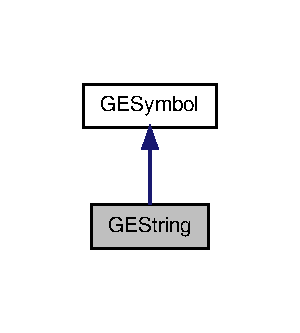
\includegraphics[width=144pt]{class_g_e_string__inherit__graph}
\end{center}
\end{figure}
\subsection*{Public Member Functions}
\begin{DoxyCompactItemize}
\item 
\hypertarget{class_g_e_string_adebf6dcc0fae4898e6dd3410447113d6}{\hyperlink{class_g_e_string_adebf6dcc0fae4898e6dd3410447113d6}{G\-E\-String} ()}\label{class_g_e_string_adebf6dcc0fae4898e6dd3410447113d6}

\begin{DoxyCompactList}\small\item\em Construct an empty Engine compatible string. \end{DoxyCompactList}\item 
\hyperlink{class_g_e_string_a7a629e649a5ec09603e839c0e0dd5e1e}{G\-E\-String} (string)
\begin{DoxyCompactList}\small\item\em Construct an Engine compatible string with the value of {\itshape data}. \end{DoxyCompactList}\item 
string \hyperlink{class_g_e_string_a7b91a6c62c744e3d05a2410b0eb90e47}{get\-Data} ()
\begin{DoxyCompactList}\small\item\em Return a copy of the data as a string. \end{DoxyCompactList}\item 
void \hyperlink{class_g_e_string_a1324fa0046f6ca0d85dc9f3298f036f1}{set\-Data} (string)
\begin{DoxyCompactList}\small\item\em Sets the data to the value of {\itshape str} \end{DoxyCompactList}\item 
virtual int \hyperlink{class_g_e_string_a7bb7b3fdc5f217ad32f6795250bdb376}{size} ()
\begin{DoxyCompactList}\small\item\em Returns the length of data. \end{DoxyCompactList}\item 
virtual void \hyperlink{class_g_e_string_a18bdaa90b17b538174ce61bb6dcc87c7}{clear} ()
\begin{DoxyCompactList}\small\item\em Sets the string to empty. \end{DoxyCompactList}\item 
\hypertarget{class_g_e_string_a058bcd0c32105659eab4194e2c9efe92}{virtual string \hyperlink{class_g_e_string_a058bcd0c32105659eab4194e2c9efe92}{to\-String} ()}\label{class_g_e_string_a058bcd0c32105659eab4194e2c9efe92}

\begin{DoxyCompactList}\small\item\em Please see \hyperlink{class_g_e_string_a7b91a6c62c744e3d05a2410b0eb90e47}{get\-Data()}. \end{DoxyCompactList}\end{DoxyCompactItemize}
\subsection*{Friends}
\begin{DoxyCompactItemize}
\item 
\hypertarget{class_g_e_string_abc89e64d0ec6c939575c3125753c6309}{class {\bfseries G\-A\-U\-S\-S}}\label{class_g_e_string_abc89e64d0ec6c939575c3125753c6309}

\end{DoxyCompactItemize}
\subsection*{Additional Inherited Members}


\subsection{Detailed Description}
\hyperlink{class_g_a_u_s_s}{G\-A\-U\-S\-S} String Symbol type. 

For all intents and purposes, this is a standard string wrapper. 

\subsection{Constructor \& Destructor Documentation}
\hypertarget{class_g_e_string_a7a629e649a5ec09603e839c0e0dd5e1e}{\index{G\-E\-String@{G\-E\-String}!G\-E\-String@{G\-E\-String}}
\index{G\-E\-String@{G\-E\-String}!GEString@{G\-E\-String}}
\subsubsection[{G\-E\-String}]{\setlength{\rightskip}{0pt plus 5cm}G\-E\-String\-::\-G\-E\-String (
\begin{DoxyParamCaption}
\item[{string}]{data}
\end{DoxyParamCaption}
)}}\label{class_g_e_string_a7a629e649a5ec09603e839c0e0dd5e1e}


Construct an Engine compatible string with the value of {\itshape data}. 

Example

\subparagraph*{Python}


\begin{DoxyCode}
1 s = \hyperlink{class_g_e_string}{GEString}(\textcolor{stringliteral}{"Hello World!"})
\end{DoxyCode}


\subparagraph*{P\-H\-P}


\begin{DoxyCode}
$s = \textcolor{keyword}{new} \hyperlink{class_g_e_string_adebf6dcc0fae4898e6dd3410447113d6}{GEString}(\textcolor{stringliteral}{"Hello World!"});
\end{DoxyCode}



\begin{DoxyParams}{Parameters}
{\em data} & User-\/defined string \\
\hline
\end{DoxyParams}


\subsection{Member Function Documentation}
\hypertarget{class_g_e_string_a18bdaa90b17b538174ce61bb6dcc87c7}{\index{G\-E\-String@{G\-E\-String}!clear@{clear}}
\index{clear@{clear}!GEString@{G\-E\-String}}
\subsubsection[{clear}]{\setlength{\rightskip}{0pt plus 5cm}virtual void G\-E\-String\-::clear (
\begin{DoxyParamCaption}
{}
\end{DoxyParamCaption}
)\hspace{0.3cm}{\ttfamily [inline]}, {\ttfamily [virtual]}}}\label{class_g_e_string_a18bdaa90b17b538174ce61bb6dcc87c7}


Sets the string to empty. 



Reimplemented from \hyperlink{class_g_e_symbol_a39d2e523aec771a73e1cc5d7a9618b88}{G\-E\-Symbol}.

\hypertarget{class_g_e_string_a7b91a6c62c744e3d05a2410b0eb90e47}{\index{G\-E\-String@{G\-E\-String}!get\-Data@{get\-Data}}
\index{get\-Data@{get\-Data}!GEString@{G\-E\-String}}
\subsubsection[{get\-Data}]{\setlength{\rightskip}{0pt plus 5cm}string G\-E\-String\-::get\-Data (
\begin{DoxyParamCaption}
{}
\end{DoxyParamCaption}
)}}\label{class_g_e_string_a7b91a6c62c744e3d05a2410b0eb90e47}


Return a copy of the data as a string. 

\subparagraph*{Python}


\begin{DoxyCode}
1 ge.executeString(\textcolor{stringliteral}{"s = \(\backslash\)"Hello World!\(\backslash\)""})
2 s = ge.getString(\textcolor{stringliteral}{"s"})
3 \textcolor{keywordflow}{print} \textcolor{stringliteral}{"s = "} + s.getData() \textcolor{comment}{# str(s) would be identical}
\end{DoxyCode}


\subparagraph*{P\-H\-P}


\begin{DoxyCode}
$ge->executeString(\textcolor{stringliteral}{"s = \(\backslash\)"Hello World!\(\backslash\)""});
$s = $ge->getString(\textcolor{stringliteral}{"s"});
echo \textcolor{stringliteral}{"s = "} . $s->getData() . PHP\_EOL; \textcolor{comment}{// Specifying '$s' would be identical}
\end{DoxyCode}
 would result in output\-: 
\begin{DoxyCode}
s = Hello World!
\end{DoxyCode}
 \hypertarget{class_g_e_string_a1324fa0046f6ca0d85dc9f3298f036f1}{\index{G\-E\-String@{G\-E\-String}!set\-Data@{set\-Data}}
\index{set\-Data@{set\-Data}!GEString@{G\-E\-String}}
\subsubsection[{set\-Data}]{\setlength{\rightskip}{0pt plus 5cm}void G\-E\-String\-::set\-Data (
\begin{DoxyParamCaption}
\item[{string}]{data}
\end{DoxyParamCaption}
)}}\label{class_g_e_string_a1324fa0046f6ca0d85dc9f3298f036f1}


Sets the data to the value of {\itshape str} 

\subparagraph*{Python}


\begin{DoxyCode}
1 s = \hyperlink{class_g_e_string}{GEString}()
2 s.setData(\textcolor{stringliteral}{"Hello World!"})
3 \textcolor{keywordflow}{print} s
\end{DoxyCode}


\subparagraph*{P\-H\-P}


\begin{DoxyCode}
$s = \textcolor{keyword}{new} \hyperlink{class_g_e_string_adebf6dcc0fae4898e6dd3410447113d6}{GEString}();
$s->setData(\textcolor{stringliteral}{"Hello World!"});
echo $s;
\end{DoxyCode}
 would result in output\-: 
\begin{DoxyCode}
Hello World!
\end{DoxyCode}
 \hypertarget{class_g_e_string_a7bb7b3fdc5f217ad32f6795250bdb376}{\index{G\-E\-String@{G\-E\-String}!size@{size}}
\index{size@{size}!GEString@{G\-E\-String}}
\subsubsection[{size}]{\setlength{\rightskip}{0pt plus 5cm}int G\-E\-String\-::size (
\begin{DoxyParamCaption}
{}
\end{DoxyParamCaption}
)\hspace{0.3cm}{\ttfamily [virtual]}}}\label{class_g_e_string_a7bb7b3fdc5f217ad32f6795250bdb376}


Returns the length of data. 

\subparagraph*{Python}


\begin{DoxyCode}
1 s = \hyperlink{class_g_e_string}{GEString}()
2 s.setData(\textcolor{stringliteral}{"Hello World!"})
3 \textcolor{keywordflow}{print} \textcolor{stringliteral}{"Length of s is "} + str(s.size()) + \textcolor{stringliteral}{" characters"}
\end{DoxyCode}


\subparagraph*{P\-H\-P}


\begin{DoxyCode}
$s = \textcolor{keyword}{new} \hyperlink{class_g_e_string_adebf6dcc0fae4898e6dd3410447113d6}{GEString}();
$s->setData(\textcolor{stringliteral}{"Hello World!"});
echo \textcolor{stringliteral}{"Length of s is "} . $s->size() . \textcolor{stringliteral}{" characters"} . PHP\_EOL;
\end{DoxyCode}
 would result in output\-: 
\begin{DoxyCode}
Length of s is 12 characters
\end{DoxyCode}
 

Reimplemented from \hyperlink{class_g_e_symbol_a706a39fc819e1c27e0d92d42c2bebcf6}{G\-E\-Symbol}.



The documentation for this class was generated from the following files\-:\begin{DoxyCompactItemize}
\item 
src/gestring.\-h\item 
src/gestring.\-cpp\end{DoxyCompactItemize}

\hypertarget{class_g_e_string_array}{\section{G\-E\-String\-Array Class Reference}
\label{class_g_e_string_array}\index{G\-E\-String\-Array@{G\-E\-String\-Array}}
}


\hyperlink{class_g_a_u_s_s}{G\-A\-U\-S\-S} String Array Symbol type.  




{\ttfamily \#include $<$gestringarray.\-h$>$}



Inheritance diagram for G\-E\-String\-Array\-:\nopagebreak
\begin{figure}[H]
\begin{center}
\leavevmode
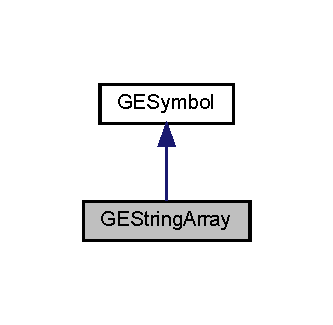
\includegraphics[width=160pt]{class_g_e_string_array__inherit__graph}
\end{center}
\end{figure}
\subsection*{Public Member Functions}
\begin{DoxyCompactItemize}
\item 
\hyperlink{class_g_e_string_array_aaf81307ac900cd22af6ced6b9ec45a0a}{G\-E\-String\-Array} (vector$<$ string $>$)
\begin{DoxyCompactList}\small\item\em Initialize a one-\/dimensional string array with a user specified vector. \end{DoxyCompactList}\item 
\hyperlink{class_g_e_string_array_abdaadc4a69d887cd739bbfc89ce60cc4}{G\-E\-String\-Array} (vector$<$ string $>$, int, int)
\begin{DoxyCompactList}\small\item\em Initialize a string array from a vector with dimensions {\itshape rows} and {\itshape cols}. \end{DoxyCompactList}\item 
string \hyperlink{class_g_e_string_array_a08286cc58c2762039163cc69a9ecf6bd}{get\-Element} (int, int)
\begin{DoxyCompactList}\small\item\em Return the string value at the {\itshape row}, {\itshape column} index. \end{DoxyCompactList}\item 
vector$<$ string $>$ \hyperlink{class_g_e_string_array_abe983e94d9cde5eecf91c04c8cf65451}{get\-Data} ()
\begin{DoxyCompactList}\small\item\em Return a collection copy of strings as a vector. \end{DoxyCompactList}\item 
void \hyperlink{class_g_e_string_array_a7af740d20e04b0d9ba770cff04b2437e}{set\-Data} (vector$<$ string $>$, int, int)
\begin{DoxyCompactList}\small\item\em Replace the contents of the string collection. \end{DoxyCompactList}\item 
bool \hyperlink{class_g_e_string_array_a0b65a5a901e490040840025322cbd731}{set\-Element} (string, int, int)
\begin{DoxyCompactList}\small\item\em Set string value to {\itshape str} at {\itshape row}, {\itshape col} element. \end{DoxyCompactList}\item 
virtual string \hyperlink{class_g_e_string_array_ab74fcbfee54edd0db02b61b299b3a7af}{to\-String} ()
\begin{DoxyCompactList}\small\item\em Returns a string representation of this object. \end{DoxyCompactList}\item 
virtual int \hyperlink{class_g_e_string_array_aa713dfa2931e223578a9fe41e3acd85d}{size} ()
\begin{DoxyCompactList}\small\item\em Return element count or in case of \hyperlink{class_g_e_string}{G\-E\-String}, string length. \end{DoxyCompactList}\item 
virtual void \hyperlink{class_g_e_string_array_a9bd5bd32a9efeb1e74128bd1d7c5c57d}{clear} ()
\begin{DoxyCompactList}\small\item\em Clear all corresponding symbol data. \end{DoxyCompactList}\end{DoxyCompactItemize}
\subsection*{Friends}
\begin{DoxyCompactItemize}
\item 
\hypertarget{class_g_e_string_array_abc89e64d0ec6c939575c3125753c6309}{class {\bfseries G\-A\-U\-S\-S}}\label{class_g_e_string_array_abc89e64d0ec6c939575c3125753c6309}

\end{DoxyCompactItemize}
\subsection*{Additional Inherited Members}


\subsection{Detailed Description}
\hyperlink{class_g_a_u_s_s}{G\-A\-U\-S\-S} String Array Symbol type. 

Represents a standard string array. Data is stored internally as a vector. 

\subsection{Constructor \& Destructor Documentation}
\hypertarget{class_g_e_string_array_aaf81307ac900cd22af6ced6b9ec45a0a}{\index{G\-E\-String\-Array@{G\-E\-String\-Array}!G\-E\-String\-Array@{G\-E\-String\-Array}}
\index{G\-E\-String\-Array@{G\-E\-String\-Array}!GEStringArray@{G\-E\-String\-Array}}
\subsubsection[{G\-E\-String\-Array}]{\setlength{\rightskip}{0pt plus 5cm}G\-E\-String\-Array\-::\-G\-E\-String\-Array (
\begin{DoxyParamCaption}
\item[{vector$<$ string $>$}]{data}
\end{DoxyParamCaption}
)}}\label{class_g_e_string_array_aaf81307ac900cd22af6ced6b9ec45a0a}


Initialize a one-\/dimensional string array with a user specified vector. 

This assumes that there are {\ttfamily data.\-size()} columns and 1 row.

Example\-:

\subparagraph*{Python}


\begin{DoxyCode}
1 sa = \hyperlink{class_g_e_string_array}{GEStringArray}([\textcolor{stringliteral}{"Open"}, \textcolor{stringliteral}{"High"}, \textcolor{stringliteral}{"Low"}])
2 \textcolor{keywordflow}{print} sa
\end{DoxyCode}


\subparagraph*{P\-H\-P}


\begin{DoxyCode}
$sa = \textcolor{keyword}{new} \hyperlink{class_g_e_string_array}{GEStringArray}(array(\textcolor{stringliteral}{"Open"}, \textcolor{stringliteral}{"High"}, \textcolor{stringliteral}{"Low"}))
echo $sa;
\end{DoxyCode}
 results in output\-: 
\begin{DoxyCode}
Open    High    Low
\end{DoxyCode}



\begin{DoxyParams}{Parameters}
{\em data} & \\
\hline
\end{DoxyParams}
\hypertarget{class_g_e_string_array_abdaadc4a69d887cd739bbfc89ce60cc4}{\index{G\-E\-String\-Array@{G\-E\-String\-Array}!G\-E\-String\-Array@{G\-E\-String\-Array}}
\index{G\-E\-String\-Array@{G\-E\-String\-Array}!GEStringArray@{G\-E\-String\-Array}}
\subsubsection[{G\-E\-String\-Array}]{\setlength{\rightskip}{0pt plus 5cm}G\-E\-String\-Array\-::\-G\-E\-String\-Array (
\begin{DoxyParamCaption}
\item[{vector$<$ string $>$}]{data, }
\item[{int}]{rows, }
\item[{int}]{cols}
\end{DoxyParamCaption}
)}}\label{class_g_e_string_array_abdaadc4a69d887cd739bbfc89ce60cc4}


Initialize a string array from a vector with dimensions {\itshape rows} and {\itshape cols}. 

Example\-:

\subparagraph*{Python}


\begin{DoxyCode}
1 sa = \hyperlink{class_g_e_string_array}{GEStringArray}([\textcolor{stringliteral}{"Open"}, \textcolor{stringliteral}{"High"}, \textcolor{stringliteral}{"Low"}, \textcolor{stringliteral}{"Close"}], 2, 2)
2 \textcolor{keywordflow}{print} sa
\end{DoxyCode}


\subparagraph*{P\-H\-P}


\begin{DoxyCode}
$sa = \textcolor{keyword}{new} \hyperlink{class_g_e_string_array}{GEStringArray}(array(\textcolor{stringliteral}{"Open"}, \textcolor{stringliteral}{"High"}, \textcolor{stringliteral}{"Low"}, \textcolor{stringliteral}{"Close"}), 2, 2);
echo $sa;
\end{DoxyCode}
 results in output\-: 
\begin{DoxyCode}
Open    High
Low     Close
\end{DoxyCode}



\begin{DoxyParams}{Parameters}
{\em data} & One-\/dimensional string data \\
\hline
{\em rows} & Row count \\
\hline
{\em cols} & Column count \\
\hline
\end{DoxyParams}


\subsection{Member Function Documentation}
\hypertarget{class_g_e_string_array_a9bd5bd32a9efeb1e74128bd1d7c5c57d}{\index{G\-E\-String\-Array@{G\-E\-String\-Array}!clear@{clear}}
\index{clear@{clear}!GEStringArray@{G\-E\-String\-Array}}
\subsubsection[{clear}]{\setlength{\rightskip}{0pt plus 5cm}virtual void G\-E\-String\-Array\-::clear (
\begin{DoxyParamCaption}
{}
\end{DoxyParamCaption}
)\hspace{0.3cm}{\ttfamily [inline]}, {\ttfamily [virtual]}}}\label{class_g_e_string_array_a9bd5bd32a9efeb1e74128bd1d7c5c57d}


Clear all corresponding symbol data. 

Does not clear from workspace. 

Reimplemented from \hyperlink{class_g_e_symbol_a39d2e523aec771a73e1cc5d7a9618b88}{G\-E\-Symbol}.

\hypertarget{class_g_e_string_array_abe983e94d9cde5eecf91c04c8cf65451}{\index{G\-E\-String\-Array@{G\-E\-String\-Array}!get\-Data@{get\-Data}}
\index{get\-Data@{get\-Data}!GEStringArray@{G\-E\-String\-Array}}
\subsubsection[{get\-Data}]{\setlength{\rightskip}{0pt plus 5cm}vector$<$ string $>$ G\-E\-String\-Array\-::get\-Data (
\begin{DoxyParamCaption}
{}
\end{DoxyParamCaption}
)}}\label{class_g_e_string_array_abe983e94d9cde5eecf91c04c8cf65451}


Return a collection copy of strings as a vector. 

Example\-:

\subparagraph*{Python}


\begin{DoxyCode}
1 \textcolor{comment}{# Create a string array using GAUSS}
2 ge.executeString(\textcolor{stringliteral}{"string sa = \{ one two three four, five six seven eight \}"})
3 
4 \textcolor{comment}{# Retrieve the string array from the symbol table}
5 sa = ge.getStringArray(\textcolor{stringliteral}{"sa"})
6 
7 \textcolor{keywordflow}{print} sa
8 \textcolor{keywordflow}{print} \textcolor{stringliteral}{" "}.join(sa.getData())
\end{DoxyCode}


\subparagraph*{P\-H\-P}


\begin{DoxyCode}
\textcolor{comment}{// Create a string array using GAUSS}
$ge->executeString(\textcolor{stringliteral}{"string sa = \{ one two three four, five six seven eight \};"});

\textcolor{comment}{// Retrieve the string array from the symbol table}
$sa = $ge->getStringArray(\textcolor{stringliteral}{"sa"});

echo $sa . PHP\_EOL;
echo implode(\textcolor{stringliteral}{" "}, $sa->getData()) . PHP\_EOL;
\end{DoxyCode}
 resulting in the output\-: 
\begin{DoxyCode}
ONE     TWO     THREE   FOUR
FIVE    SIX     SEVEN   EIGHT

ONE TWO THREE FOUR FIVE SIX SEVEN EIGHT
\end{DoxyCode}


\begin{DoxyReturn}{Returns}
string vector 
\end{DoxyReturn}
\hypertarget{class_g_e_string_array_a08286cc58c2762039163cc69a9ecf6bd}{\index{G\-E\-String\-Array@{G\-E\-String\-Array}!get\-Element@{get\-Element}}
\index{get\-Element@{get\-Element}!GEStringArray@{G\-E\-String\-Array}}
\subsubsection[{get\-Element}]{\setlength{\rightskip}{0pt plus 5cm}string G\-E\-String\-Array\-::get\-Element (
\begin{DoxyParamCaption}
\item[{int}]{row, }
\item[{int}]{col}
\end{DoxyParamCaption}
)}}\label{class_g_e_string_array_a08286cc58c2762039163cc69a9ecf6bd}


Return the string value at the {\itshape row}, {\itshape column} index. 

Example\-:

\subparagraph*{Python}


\begin{DoxyCode}
1 sa = \hyperlink{class_g_e_string_array}{GEStringArray}([\textcolor{stringliteral}{"foo"}, \textcolor{stringliteral}{"bar"}, \textcolor{stringliteral}{"baz"}])
2 \textcolor{keywordflow}{print} str(sa.getElement(0, 1))
\end{DoxyCode}


\subparagraph*{P\-H\-P}


\begin{DoxyCode}
$sa = \textcolor{keyword}{new} \hyperlink{class_g_e_string_array}{GEStringArray}(array(\textcolor{stringliteral}{"foo"}, \textcolor{stringliteral}{"bar"}, \textcolor{stringliteral}{"baz"}));
echo $sa->getElement(0, 1);
\end{DoxyCode}
 results in the output\-: 
\begin{DoxyCode}
bar
\end{DoxyCode}



\begin{DoxyParams}{Parameters}
{\em row} & Row index \\
\hline
{\em col} & Column index \\
\hline
\end{DoxyParams}
\begin{DoxyReturn}{Returns}
Value at specified index 
\end{DoxyReturn}
\hypertarget{class_g_e_string_array_a7af740d20e04b0d9ba770cff04b2437e}{\index{G\-E\-String\-Array@{G\-E\-String\-Array}!set\-Data@{set\-Data}}
\index{set\-Data@{set\-Data}!GEStringArray@{G\-E\-String\-Array}}
\subsubsection[{set\-Data}]{\setlength{\rightskip}{0pt plus 5cm}void G\-E\-String\-Array\-::set\-Data (
\begin{DoxyParamCaption}
\item[{vector$<$ string $>$}]{data, }
\item[{int}]{rows, }
\item[{int}]{cols}
\end{DoxyParamCaption}
)}}\label{class_g_e_string_array_a7af740d20e04b0d9ba770cff04b2437e}


Replace the contents of the string collection. 

The length of {\itshape data} should be equal to {\itshape rows} $\ast$ {\itshape cols}.


\begin{DoxyParams}{Parameters}
{\em rows} & Rows \\
\hline
{\em cols} & Cols \\
\hline
\end{DoxyParams}
\hypertarget{class_g_e_string_array_a0b65a5a901e490040840025322cbd731}{\index{G\-E\-String\-Array@{G\-E\-String\-Array}!set\-Element@{set\-Element}}
\index{set\-Element@{set\-Element}!GEStringArray@{G\-E\-String\-Array}}
\subsubsection[{set\-Element}]{\setlength{\rightskip}{0pt plus 5cm}bool G\-E\-String\-Array\-::set\-Element (
\begin{DoxyParamCaption}
\item[{string}]{str, }
\item[{int}]{row, }
\item[{int}]{col}
\end{DoxyParamCaption}
)}}\label{class_g_e_string_array_a0b65a5a901e490040840025322cbd731}


Set string value to {\itshape str} at {\itshape row}, {\itshape col} element. 

Example\-:

\subparagraph*{Python}


\begin{DoxyCode}
1 sa = \hyperlink{class_g_e_string_array}{GEStringArray}([\textcolor{stringliteral}{"foo"}, \textcolor{stringliteral}{"bar"}, \textcolor{stringliteral}{"baz"}])
2 sa.setElement(\textcolor{stringliteral}{"foo"}, 0, 1)
3 \textcolor{keywordflow}{print} sa
\end{DoxyCode}


\subparagraph*{P\-H\-P}


\begin{DoxyCode}
$sa = \textcolor{keyword}{new} \hyperlink{class_g_e_string_array}{GEStringArray}(array(\textcolor{stringliteral}{"foo"}, \textcolor{stringliteral}{"bar"}, \textcolor{stringliteral}{"baz"}));
$sa->setElement(\textcolor{stringliteral}{"foo"}, 0, 1);
echo $sa->toString();
\end{DoxyCode}
 results in the output\-: 
\begin{DoxyCode}
foo foo baz
\end{DoxyCode}



\begin{DoxyParams}{Parameters}
{\em row} & Row \\
\hline
{\em col} & Col \\
\hline
\end{DoxyParams}
\hypertarget{class_g_e_string_array_aa713dfa2931e223578a9fe41e3acd85d}{\index{G\-E\-String\-Array@{G\-E\-String\-Array}!size@{size}}
\index{size@{size}!GEStringArray@{G\-E\-String\-Array}}
\subsubsection[{size}]{\setlength{\rightskip}{0pt plus 5cm}virtual int G\-E\-String\-Array\-::size (
\begin{DoxyParamCaption}
{}
\end{DoxyParamCaption}
)\hspace{0.3cm}{\ttfamily [inline]}, {\ttfamily [virtual]}}}\label{class_g_e_string_array_aa713dfa2931e223578a9fe41e3acd85d}


Return element count or in case of \hyperlink{class_g_e_string}{G\-E\-String}, string length. 

Returns the total element count for the data.

\begin{DoxyReturn}{Returns}
Total element count 
\end{DoxyReturn}


Reimplemented from \hyperlink{class_g_e_symbol_a706a39fc819e1c27e0d92d42c2bebcf6}{G\-E\-Symbol}.

\hypertarget{class_g_e_string_array_ab74fcbfee54edd0db02b61b299b3a7af}{\index{G\-E\-String\-Array@{G\-E\-String\-Array}!to\-String@{to\-String}}
\index{to\-String@{to\-String}!GEStringArray@{G\-E\-String\-Array}}
\subsubsection[{to\-String}]{\setlength{\rightskip}{0pt plus 5cm}string G\-E\-String\-Array\-::to\-String (
\begin{DoxyParamCaption}
{}
\end{DoxyParamCaption}
)\hspace{0.3cm}{\ttfamily [virtual]}}}\label{class_g_e_string_array_ab74fcbfee54edd0db02b61b299b3a7af}


Returns a string representation of this object. 



Reimplemented from \hyperlink{class_g_e_symbol_a6790ac75620cc1a9e37d67279e8bd4d1}{G\-E\-Symbol}.



The documentation for this class was generated from the following files\-:\begin{DoxyCompactItemize}
\item 
src/gestringarray.\-h\item 
src/gestringarray.\-cpp\end{DoxyCompactItemize}

\hypertarget{class_g_e_symbol}{\section{G\-E\-Symbol Class Reference}
\label{class_g_e_symbol}\index{G\-E\-Symbol@{G\-E\-Symbol}}
}


Abstract parent class for all symbol types.  




{\ttfamily \#include $<$gesymbol.\-h$>$}



Inheritance diagram for G\-E\-Symbol\-:
\nopagebreak
\begin{figure}[H]
\begin{center}
\leavevmode
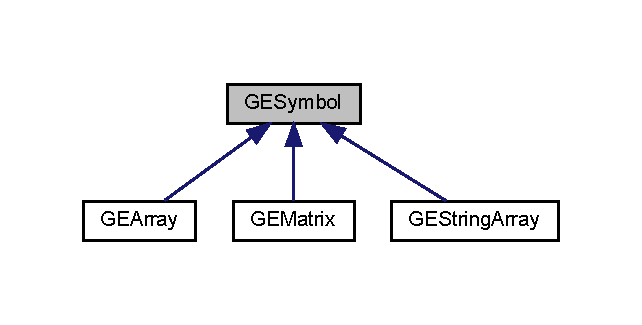
\includegraphics[width=308pt]{class_g_e_symbol__inherit__graph}
\end{center}
\end{figure}
\subsection*{Public Member Functions}
\begin{DoxyCompactItemize}
\item 
virtual int \hyperlink{class_g_e_symbol_a470e7764dc5d1a68e991fd75f64861e9}{get\-Rows} () const 
\begin{DoxyCompactList}\small\item\em Return row count. \end{DoxyCompactList}\item 
virtual int \hyperlink{class_g_e_symbol_a39fa2193c2edfdd0fb062472fd4a445d}{get\-Cols} () const 
\begin{DoxyCompactList}\small\item\em Return column count. \end{DoxyCompactList}\item 
virtual bool \hyperlink{class_g_e_symbol_af65ad912b91392ff60dcfa002878a3c4}{is\-Complex} () const 
\begin{DoxyCompactList}\small\item\em Return if data is complex. \end{DoxyCompactList}\item 
virtual int \hyperlink{class_g_e_symbol_a9dfb28fc5c1a67658c5380d5fbdfbc24}{size} () const 
\begin{DoxyCompactList}\small\item\em Return element count. \end{DoxyCompactList}\item 
virtual void \hyperlink{class_g_e_symbol_a39d2e523aec771a73e1cc5d7a9618b88}{clear} ()
\begin{DoxyCompactList}\small\item\em Clear all corresponding symbol data. \end{DoxyCompactList}\item 
virtual string \hyperlink{class_g_e_symbol_ac79ba555226072d4b03f06e9f8bb6afb}{to\-String} () const 
\begin{DoxyCompactList}\small\item\em Returns a string representation of this object. \end{DoxyCompactList}\item 
\hypertarget{class_g_e_symbol_ad1959d131a38822003f597fb977d80e4}{int {\bfseries type} () const }\label{class_g_e_symbol_ad1959d131a38822003f597fb977d80e4}

\end{DoxyCompactItemize}
\subsection*{Protected Member Functions}
\begin{DoxyCompactItemize}
\item 
\hypertarget{class_g_e_symbol_a8bec3b923598e9daab2aab824a619db5}{{\bfseries G\-E\-Symbol} (int type)}\label{class_g_e_symbol_a8bec3b923598e9daab2aab824a619db5}

\item 
\hypertarget{class_g_e_symbol_a8f5a7ba90f2d124529d6b9d7aa59cb59}{virtual void {\bfseries set\-Rows} (int)}\label{class_g_e_symbol_a8f5a7ba90f2d124529d6b9d7aa59cb59}

\item 
\hypertarget{class_g_e_symbol_a5de6b791c1f11ef2a18e5e6335f1731e}{virtual void {\bfseries set\-Cols} (int)}\label{class_g_e_symbol_a5de6b791c1f11ef2a18e5e6335f1731e}

\item 
\hypertarget{class_g_e_symbol_abc3312d19d04a1eef62c0c4d255924df}{virtual void {\bfseries set\-Complex} (bool)}\label{class_g_e_symbol_abc3312d19d04a1eef62c0c4d255924df}

\end{DoxyCompactItemize}
\subsection*{Protected Attributes}
\begin{DoxyCompactItemize}
\item 
\hypertarget{class_g_e_symbol_a36b478c80c6b652753f2b125d2de596a}{int {\bfseries rows\-\_\-}}\label{class_g_e_symbol_a36b478c80c6b652753f2b125d2de596a}

\item 
\hypertarget{class_g_e_symbol_ad6fa1f94281aebfc239e73aaefa34866}{int {\bfseries cols\-\_\-}}\label{class_g_e_symbol_ad6fa1f94281aebfc239e73aaefa34866}

\item 
\hypertarget{class_g_e_symbol_a8ad78c322adee566f1180f9d9b359798}{bool {\bfseries complex\-\_\-}}\label{class_g_e_symbol_a8ad78c322adee566f1180f9d9b359798}

\item 
\hypertarget{class_g_e_symbol_a0cc2349d51f6c7111f79755761f86f01}{int {\bfseries type\-\_\-}}\label{class_g_e_symbol_a0cc2349d51f6c7111f79755761f86f01}

\end{DoxyCompactItemize}


\subsection{Detailed Description}
Abstract parent class for all symbol types. 

\subsection{Member Function Documentation}
\hypertarget{class_g_e_symbol_a39d2e523aec771a73e1cc5d7a9618b88}{\index{G\-E\-Symbol@{G\-E\-Symbol}!clear@{clear}}
\index{clear@{clear}!GESymbol@{G\-E\-Symbol}}
\subsubsection[{clear}]{\setlength{\rightskip}{0pt plus 5cm}virtual void G\-E\-Symbol\-::clear (
\begin{DoxyParamCaption}
{}
\end{DoxyParamCaption}
)\hspace{0.3cm}{\ttfamily [inline]}, {\ttfamily [virtual]}}}\label{class_g_e_symbol_a39d2e523aec771a73e1cc5d7a9618b88}


Clear all corresponding symbol data. 

Does not clear from workspace. 

Reimplemented in \hyperlink{class_g_e_matrix_a1bf6ddd9f46248e1c03c0d952d572103}{G\-E\-Matrix}, \hyperlink{class_g_e_array_ad7fd6880da03d11c13387ea9e1e1cd5d}{G\-E\-Array}, and \hyperlink{class_g_e_string_array_a9bd5bd32a9efeb1e74128bd1d7c5c57d}{G\-E\-String\-Array}.

\hypertarget{class_g_e_symbol_a39fa2193c2edfdd0fb062472fd4a445d}{\index{G\-E\-Symbol@{G\-E\-Symbol}!get\-Cols@{get\-Cols}}
\index{get\-Cols@{get\-Cols}!GESymbol@{G\-E\-Symbol}}
\subsubsection[{get\-Cols}]{\setlength{\rightskip}{0pt plus 5cm}int G\-E\-Symbol\-::get\-Cols (
\begin{DoxyParamCaption}
{}
\end{DoxyParamCaption}
) const\hspace{0.3cm}{\ttfamily [virtual]}}}\label{class_g_e_symbol_a39fa2193c2edfdd0fb062472fd4a445d}


Return column count. 

Returns the column count.

\begin{DoxyReturn}{Returns}
Column count 
\end{DoxyReturn}
\hypertarget{class_g_e_symbol_a470e7764dc5d1a68e991fd75f64861e9}{\index{G\-E\-Symbol@{G\-E\-Symbol}!get\-Rows@{get\-Rows}}
\index{get\-Rows@{get\-Rows}!GESymbol@{G\-E\-Symbol}}
\subsubsection[{get\-Rows}]{\setlength{\rightskip}{0pt plus 5cm}int G\-E\-Symbol\-::get\-Rows (
\begin{DoxyParamCaption}
{}
\end{DoxyParamCaption}
) const\hspace{0.3cm}{\ttfamily [virtual]}}}\label{class_g_e_symbol_a470e7764dc5d1a68e991fd75f64861e9}


Return row count. 

Returns the row count.

\begin{DoxyReturn}{Returns}
Row count 
\end{DoxyReturn}
\hypertarget{class_g_e_symbol_af65ad912b91392ff60dcfa002878a3c4}{\index{G\-E\-Symbol@{G\-E\-Symbol}!is\-Complex@{is\-Complex}}
\index{is\-Complex@{is\-Complex}!GESymbol@{G\-E\-Symbol}}
\subsubsection[{is\-Complex}]{\setlength{\rightskip}{0pt plus 5cm}bool G\-E\-Symbol\-::is\-Complex (
\begin{DoxyParamCaption}
{}
\end{DoxyParamCaption}
) const\hspace{0.3cm}{\ttfamily [virtual]}}}\label{class_g_e_symbol_af65ad912b91392ff60dcfa002878a3c4}


Return if data is complex. 

Returns whether or not the data is complex or not.

Applies to \hyperlink{class_g_e_array}{G\-E\-Array} and \hyperlink{class_g_e_matrix}{G\-E\-Matrix} only.

\begin{DoxyReturn}{Returns}
True if data is complex, false if not. 
\end{DoxyReturn}
\hypertarget{class_g_e_symbol_a9dfb28fc5c1a67658c5380d5fbdfbc24}{\index{G\-E\-Symbol@{G\-E\-Symbol}!size@{size}}
\index{size@{size}!GESymbol@{G\-E\-Symbol}}
\subsubsection[{size}]{\setlength{\rightskip}{0pt plus 5cm}int G\-E\-Symbol\-::size (
\begin{DoxyParamCaption}
{}
\end{DoxyParamCaption}
) const\hspace{0.3cm}{\ttfamily [virtual]}}}\label{class_g_e_symbol_a9dfb28fc5c1a67658c5380d5fbdfbc24}


Return element count. 

Returns the total element count for the data.

\begin{DoxyReturn}{Returns}
Total element count 
\end{DoxyReturn}


Reimplemented in \hyperlink{class_g_e_string_array_aab1e6ad88ece669100fab114efe43b43}{G\-E\-String\-Array}, and \hyperlink{class_g_e_array_a4030556e997a324e09abcf46e6a9e7ef}{G\-E\-Array}.

\hypertarget{class_g_e_symbol_ac79ba555226072d4b03f06e9f8bb6afb}{\index{G\-E\-Symbol@{G\-E\-Symbol}!to\-String@{to\-String}}
\index{to\-String@{to\-String}!GESymbol@{G\-E\-Symbol}}
\subsubsection[{to\-String}]{\setlength{\rightskip}{0pt plus 5cm}virtual string G\-E\-Symbol\-::to\-String (
\begin{DoxyParamCaption}
{}
\end{DoxyParamCaption}
) const\hspace{0.3cm}{\ttfamily [inline]}, {\ttfamily [virtual]}}}\label{class_g_e_symbol_ac79ba555226072d4b03f06e9f8bb6afb}


Returns a string representation of this object. 



Reimplemented in \hyperlink{class_g_e_matrix_af17030b3ac740673ebe81612d9fe5963}{G\-E\-Matrix}, \hyperlink{class_g_e_array_a9f0f5b80ff919ebbf663e0e2ad257512}{G\-E\-Array}, and \hyperlink{class_g_e_string_array_af561837dd261d89c356d1c9cf428b1d5}{G\-E\-String\-Array}.



The documentation for this class was generated from the following files\-:\begin{DoxyCompactItemize}
\item 
src/gesymbol.\-h\item 
src/gesymbol.\-cpp\end{DoxyCompactItemize}

\hypertarget{struct_g_e_sym_type}{\section{G\-E\-Sym\-Type Struct Reference}
\label{struct_g_e_sym_type}\index{G\-E\-Sym\-Type@{G\-E\-Sym\-Type}}
}


\hyperlink{struct_g_e_sym_type}{G\-E\-Sym\-Type} stores \hyperlink{class_g_a_u_s_s}{G\-A\-U\-S\-S} constant values for different symbol types.  




{\ttfamily \#include $<$gesymtype.\-h$>$}

\subsection*{Public Types}
\begin{DoxyCompactItemize}
\item 
enum \hyperlink{struct_g_e_sym_type_a05477e08255bea70296f7825493e95fc}{S\-Y\-M\-T\-Y\-P\-E} \{ \\*
\hyperlink{struct_g_e_sym_type_a05477e08255bea70296f7825493e95fca0e3633d8cf7dbbdbe3b45bdd24cae7b0}{S\-C\-A\-L\-A\-R} = 16, 
\hyperlink{struct_g_e_sym_type_a05477e08255bea70296f7825493e95fcaaf5984cc491fc4b4fcf2162f18f0272c}{S\-P\-A\-R\-S\-E} = 38, 
\hyperlink{struct_g_e_sym_type_a05477e08255bea70296f7825493e95fcace35d10ede406b8a2768ddac17b1d22c}{M\-A\-T\-R\-I\-X} = 6, 
\hyperlink{struct_g_e_sym_type_a05477e08255bea70296f7825493e95fcad7b91a02b7bd02be62866581fb00ab77}{S\-T\-R\-I\-N\-G} = 13, 
\\*
\hyperlink{struct_g_e_sym_type_a05477e08255bea70296f7825493e95fcad16784afa03e303f68740a9a33dc887b}{S\-T\-R\-U\-C\-T} = 19, 
\hyperlink{struct_g_e_sym_type_a05477e08255bea70296f7825493e95fcab84d43f39e58b9cd3995b3aafc7239d6}{P\-S\-T\-R\-U\-C\-T} = 23, 
\hyperlink{struct_g_e_sym_type_a05477e08255bea70296f7825493e95fcadba1b6c2cd5c27167323652b1c23c9e0}{S\-T\-R\-I\-N\-G\-\_\-\-A\-R\-R\-A\-Y} = 15, 
\hyperlink{struct_g_e_sym_type_a05477e08255bea70296f7825493e95fcad3f85fecfcee857d9b08cf4ebe77c32f}{A\-R\-R\-A\-Y\-\_\-\-G\-A\-U\-S\-S} = 17, 
\\*
\hyperlink{struct_g_e_sym_type_a05477e08255bea70296f7825493e95fca4793088111ff7058b2bd6e4bde07f816}{P\-R\-O\-C} = 8, 
\hyperlink{struct_g_e_sym_type_a05477e08255bea70296f7825493e95fca7d507081df635250120e56c8766ec504}{O\-T\-H\-E\-R} = 99
 \}
\begin{DoxyCompactList}\small\item\em Enumeration of all symbol types known to \hyperlink{class_g_a_u_s_s}{G\-A\-U\-S\-S}. \end{DoxyCompactList}\end{DoxyCompactItemize}


\subsection{Detailed Description}
\hyperlink{struct_g_e_sym_type}{G\-E\-Sym\-Type} stores \hyperlink{class_g_a_u_s_s}{G\-A\-U\-S\-S} constant values for different symbol types. 

Access these in a static fashion.

Example\-:

\subparagraph*{Python}


\begin{DoxyCode}
1 \textcolor{keyword}{def }checkType(x):
2     \textcolor{keywordflow}{return} \{
3         GESymType.SCALAR:
4             \textcolor{stringliteral}{"Symbol is a scalar."},
5         GESymType.SPARSE:
6             \textcolor{stringliteral}{"Symbol is a sparse matrix."},
7         GESymType.MATRIX:
8             \textcolor{stringliteral}{"Symbol is a matrix."},
9         GESymType.STRING:
10             \textcolor{stringliteral}{"Symbol is a string."},
11         GESymType.STRUCT:
12             \textcolor{stringliteral}{"Symbol is a struct."},
13         GESymType.STRING\_ARRAY:
14             \textcolor{stringliteral}{"Symbol is a string array."},
15         GESymType.ARRAY\_GAUSS:
16             \textcolor{stringliteral}{"Symbol is an array."},
17         GESymType.PROC:
18             \textcolor{stringliteral}{"Symbol is a proc."},
19         GESymType.OTHER:
20             \textcolor{stringliteral}{"Symbol is of another type."}
21 
22         \}.get(x, \textcolor{stringliteral}{"Unknown symbol type"})
23 
24 ge.executeString(\textcolor{stringliteral}{"x = 1.0"})
25 ge.executeString(\textcolor{stringliteral}{"s = \(\backslash\)"test\(\backslash\)""})
26 ge.executeString(\textcolor{stringliteral}{"a = areshape(seqa(1, 1, 24), 2|3|4)"})
27 
28 xType = ge.getSymbolType(\textcolor{stringliteral}{"x"})
29 sType = ge.getSymbolType(\textcolor{stringliteral}{"s"})
30 aType = ge.getSymbolType(\textcolor{stringliteral}{"a"})
31 
32 \textcolor{keywordflow}{print} checkType(xType)
33 \textcolor{keywordflow}{print} checkType(sType)
34 \textcolor{keywordflow}{print} checkType(aType)
\end{DoxyCode}
 \subparagraph*{P\-H\-P}


\begin{DoxyCode}
\textcolor{keyword}{function} checkType($type) \{
    \textcolor{keywordflow}{switch} ($type) \{
        \textcolor{keywordflow}{case} \hyperlink{struct_g_e_sym_type_a05477e08255bea70296f7825493e95fca0e3633d8cf7dbbdbe3b45bdd24cae7b0}{GESymType::SCALAR}:
            \textcolor{keywordflow}{return} \textcolor{stringliteral}{"Symbol is a scalar."};
            \textcolor{keywordflow}{break};
        \textcolor{keywordflow}{case} \hyperlink{struct_g_e_sym_type_a05477e08255bea70296f7825493e95fcaaf5984cc491fc4b4fcf2162f18f0272c}{GESymType::SPARSE}:
            \textcolor{keywordflow}{return} \textcolor{stringliteral}{"Symbol is a sparse matrix."};
            \textcolor{keywordflow}{break};
        \textcolor{keywordflow}{case} \hyperlink{struct_g_e_sym_type_a05477e08255bea70296f7825493e95fcace35d10ede406b8a2768ddac17b1d22c}{GESymType::MATRIX}:
            \textcolor{keywordflow}{return} \textcolor{stringliteral}{"Symbol is a matrix."};
            \textcolor{keywordflow}{break};
        \textcolor{keywordflow}{case} \hyperlink{struct_g_e_sym_type_a05477e08255bea70296f7825493e95fcad7b91a02b7bd02be62866581fb00ab77}{GESymType::STRING}:
            \textcolor{keywordflow}{return} \textcolor{stringliteral}{"Symbol is a string."};
            \textcolor{keywordflow}{break};
        \textcolor{keywordflow}{case} \hyperlink{struct_g_e_sym_type_a05477e08255bea70296f7825493e95fcad16784afa03e303f68740a9a33dc887b}{GESymType::STRUCT}:
            \textcolor{keywordflow}{return} \textcolor{stringliteral}{"Symbol is a struct."};
            \textcolor{keywordflow}{break};
        \textcolor{keywordflow}{case} \hyperlink{struct_g_e_sym_type_a05477e08255bea70296f7825493e95fcadba1b6c2cd5c27167323652b1c23c9e0}{GESymType::STRING\_ARRAY}:
            \textcolor{keywordflow}{return} \textcolor{stringliteral}{"Symbol is a string array."};
            \textcolor{keywordflow}{break};
        \textcolor{keywordflow}{case} \hyperlink{struct_g_e_sym_type_a05477e08255bea70296f7825493e95fcad3f85fecfcee857d9b08cf4ebe77c32f}{GESymType::ARRAY\_GAUSS}:
            \textcolor{keywordflow}{return} \textcolor{stringliteral}{"Symbol is an array."};
            \textcolor{keywordflow}{break};
        \textcolor{keywordflow}{case} \hyperlink{struct_g_e_sym_type_a05477e08255bea70296f7825493e95fca4793088111ff7058b2bd6e4bde07f816}{GESymType::PROC}:
            \textcolor{keywordflow}{return} \textcolor{stringliteral}{"Symbol is a proc."};
            \textcolor{keywordflow}{break};
        \textcolor{keywordflow}{case} \hyperlink{struct_g_e_sym_type_a05477e08255bea70296f7825493e95fca7d507081df635250120e56c8766ec504}{GESymType::OTHER}:
            \textcolor{keywordflow}{return} \textcolor{stringliteral}{"Symbol is of another type."};
            \textcolor{keywordflow}{break};
        \textcolor{keywordflow}{default}:
            \textcolor{keywordflow}{return} \textcolor{stringliteral}{"Unknown symbol type"};
    \}
\}

$ge->executeString(\textcolor{stringliteral}{"x = 1.0;"});
$ge->executeString(\textcolor{stringliteral}{"s = \(\backslash\)"test\(\backslash\)";"});
$ge->executeString(\textcolor{stringliteral}{"a = areshape(seqa(1, 1, 24), 2|3|4);"});

$xType = $ge->getSymbolType(\textcolor{stringliteral}{"x"});
$sType = $ge->getSymbolType(\textcolor{stringliteral}{"s"});
$aType = $ge->getSymbolType(\textcolor{stringliteral}{"a"});

echo checkType($xType) . PHP\_EOL;
echo checkType($sType) . PHP\_EOL;
echo checkType($aType) . PHP\_EOL;
\end{DoxyCode}
 results in output\-: 
\begin{DoxyCode}
Symbol is a matrix.
Symbol is a \textcolor{keywordtype}{string}.
Symbol is an array.
\end{DoxyCode}
 

\subsection{Member Enumeration Documentation}
\hypertarget{struct_g_e_sym_type_a05477e08255bea70296f7825493e95fc}{\index{G\-E\-Sym\-Type@{G\-E\-Sym\-Type}!S\-Y\-M\-T\-Y\-P\-E@{S\-Y\-M\-T\-Y\-P\-E}}
\index{S\-Y\-M\-T\-Y\-P\-E@{S\-Y\-M\-T\-Y\-P\-E}!GESymType@{G\-E\-Sym\-Type}}
\subsubsection[{S\-Y\-M\-T\-Y\-P\-E}]{\setlength{\rightskip}{0pt plus 5cm}enum {\bf G\-E\-Sym\-Type\-::\-S\-Y\-M\-T\-Y\-P\-E}}}\label{struct_g_e_sym_type_a05477e08255bea70296f7825493e95fc}


Enumeration of all symbol types known to \hyperlink{class_g_a_u_s_s}{G\-A\-U\-S\-S}. 

\begin{Desc}
\item[Enumerator]\par
\begin{description}
\index{S\-C\-A\-L\-A\-R@{S\-C\-A\-L\-A\-R}!G\-E\-Sym\-Type@{G\-E\-Sym\-Type}}\index{G\-E\-Sym\-Type@{G\-E\-Sym\-Type}!S\-C\-A\-L\-A\-R@{S\-C\-A\-L\-A\-R}}\item[{\em 
\hypertarget{struct_g_e_sym_type_a05477e08255bea70296f7825493e95fca0e3633d8cf7dbbdbe3b45bdd24cae7b0}{S\-C\-A\-L\-A\-R}\label{struct_g_e_sym_type_a05477e08255bea70296f7825493e95fca0e3633d8cf7dbbdbe3b45bdd24cae7b0}
}]Scalar (i.\-e. 1, 1.\-5); \index{S\-P\-A\-R\-S\-E@{S\-P\-A\-R\-S\-E}!G\-E\-Sym\-Type@{G\-E\-Sym\-Type}}\index{G\-E\-Sym\-Type@{G\-E\-Sym\-Type}!S\-P\-A\-R\-S\-E@{S\-P\-A\-R\-S\-E}}\item[{\em 
\hypertarget{struct_g_e_sym_type_a05477e08255bea70296f7825493e95fcaaf5984cc491fc4b4fcf2162f18f0272c}{S\-P\-A\-R\-S\-E}\label{struct_g_e_sym_type_a05477e08255bea70296f7825493e95fcaaf5984cc491fc4b4fcf2162f18f0272c}
}]Sparse Matrix. \index{M\-A\-T\-R\-I\-X@{M\-A\-T\-R\-I\-X}!G\-E\-Sym\-Type@{G\-E\-Sym\-Type}}\index{G\-E\-Sym\-Type@{G\-E\-Sym\-Type}!M\-A\-T\-R\-I\-X@{M\-A\-T\-R\-I\-X}}\item[{\em 
\hypertarget{struct_g_e_sym_type_a05477e08255bea70296f7825493e95fcace35d10ede406b8a2768ddac17b1d22c}{M\-A\-T\-R\-I\-X}\label{struct_g_e_sym_type_a05477e08255bea70296f7825493e95fcace35d10ede406b8a2768ddac17b1d22c}
}]Matrix. \index{S\-T\-R\-I\-N\-G@{S\-T\-R\-I\-N\-G}!G\-E\-Sym\-Type@{G\-E\-Sym\-Type}}\index{G\-E\-Sym\-Type@{G\-E\-Sym\-Type}!S\-T\-R\-I\-N\-G@{S\-T\-R\-I\-N\-G}}\item[{\em 
\hypertarget{struct_g_e_sym_type_a05477e08255bea70296f7825493e95fcad7b91a02b7bd02be62866581fb00ab77}{S\-T\-R\-I\-N\-G}\label{struct_g_e_sym_type_a05477e08255bea70296f7825493e95fcad7b91a02b7bd02be62866581fb00ab77}
}]String. \index{S\-T\-R\-U\-C\-T@{S\-T\-R\-U\-C\-T}!G\-E\-Sym\-Type@{G\-E\-Sym\-Type}}\index{G\-E\-Sym\-Type@{G\-E\-Sym\-Type}!S\-T\-R\-U\-C\-T@{S\-T\-R\-U\-C\-T}}\item[{\em 
\hypertarget{struct_g_e_sym_type_a05477e08255bea70296f7825493e95fcad16784afa03e303f68740a9a33dc887b}{S\-T\-R\-U\-C\-T}\label{struct_g_e_sym_type_a05477e08255bea70296f7825493e95fcad16784afa03e303f68740a9a33dc887b}
}]Structure. \index{P\-S\-T\-R\-U\-C\-T@{P\-S\-T\-R\-U\-C\-T}!G\-E\-Sym\-Type@{G\-E\-Sym\-Type}}\index{G\-E\-Sym\-Type@{G\-E\-Sym\-Type}!P\-S\-T\-R\-U\-C\-T@{P\-S\-T\-R\-U\-C\-T}}\item[{\em 
\hypertarget{struct_g_e_sym_type_a05477e08255bea70296f7825493e95fcab84d43f39e58b9cd3995b3aafc7239d6}{P\-S\-T\-R\-U\-C\-T}\label{struct_g_e_sym_type_a05477e08255bea70296f7825493e95fcab84d43f39e58b9cd3995b3aafc7239d6}
}]P\-Struct. \index{S\-T\-R\-I\-N\-G\-\_\-\-A\-R\-R\-A\-Y@{S\-T\-R\-I\-N\-G\-\_\-\-A\-R\-R\-A\-Y}!G\-E\-Sym\-Type@{G\-E\-Sym\-Type}}\index{G\-E\-Sym\-Type@{G\-E\-Sym\-Type}!S\-T\-R\-I\-N\-G\-\_\-\-A\-R\-R\-A\-Y@{S\-T\-R\-I\-N\-G\-\_\-\-A\-R\-R\-A\-Y}}\item[{\em 
\hypertarget{struct_g_e_sym_type_a05477e08255bea70296f7825493e95fcadba1b6c2cd5c27167323652b1c23c9e0}{S\-T\-R\-I\-N\-G\-\_\-\-A\-R\-R\-A\-Y}\label{struct_g_e_sym_type_a05477e08255bea70296f7825493e95fcadba1b6c2cd5c27167323652b1c23c9e0}
}]String Array. \index{A\-R\-R\-A\-Y\-\_\-\-G\-A\-U\-S\-S@{A\-R\-R\-A\-Y\-\_\-\-G\-A\-U\-S\-S}!G\-E\-Sym\-Type@{G\-E\-Sym\-Type}}\index{G\-E\-Sym\-Type@{G\-E\-Sym\-Type}!A\-R\-R\-A\-Y\-\_\-\-G\-A\-U\-S\-S@{A\-R\-R\-A\-Y\-\_\-\-G\-A\-U\-S\-S}}\item[{\em 
\hypertarget{struct_g_e_sym_type_a05477e08255bea70296f7825493e95fcad3f85fecfcee857d9b08cf4ebe77c32f}{A\-R\-R\-A\-Y\-\_\-\-G\-A\-U\-S\-S}\label{struct_g_e_sym_type_a05477e08255bea70296f7825493e95fcad3f85fecfcee857d9b08cf4ebe77c32f}
}]N-\/\-Dimensional Array. \index{P\-R\-O\-C@{P\-R\-O\-C}!G\-E\-Sym\-Type@{G\-E\-Sym\-Type}}\index{G\-E\-Sym\-Type@{G\-E\-Sym\-Type}!P\-R\-O\-C@{P\-R\-O\-C}}\item[{\em 
\hypertarget{struct_g_e_sym_type_a05477e08255bea70296f7825493e95fca4793088111ff7058b2bd6e4bde07f816}{P\-R\-O\-C}\label{struct_g_e_sym_type_a05477e08255bea70296f7825493e95fca4793088111ff7058b2bd6e4bde07f816}
}]Proc. \index{O\-T\-H\-E\-R@{O\-T\-H\-E\-R}!G\-E\-Sym\-Type@{G\-E\-Sym\-Type}}\index{G\-E\-Sym\-Type@{G\-E\-Sym\-Type}!O\-T\-H\-E\-R@{O\-T\-H\-E\-R}}\item[{\em 
\hypertarget{struct_g_e_sym_type_a05477e08255bea70296f7825493e95fca7d507081df635250120e56c8766ec504}{O\-T\-H\-E\-R}\label{struct_g_e_sym_type_a05477e08255bea70296f7825493e95fca7d507081df635250120e56c8766ec504}
}]Other. \end{description}
\end{Desc}


The documentation for this struct was generated from the following file\-:\begin{DoxyCompactItemize}
\item 
src/gesymtype.\-h\end{DoxyCompactItemize}

\hypertarget{class_g_e_workspace}{\section{G\-E\-Workspace Class Reference}
\label{class_g_e_workspace}\index{G\-E\-Workspace@{G\-E\-Workspace}}
}


Wrapper for a Workspace\-Handle\-\_\-t$\ast$ object.  




{\ttfamily \#include $<$geworkspace.\-h$>$}

\subsection*{Public Member Functions}
\begin{DoxyCompactItemize}
\item 
\hypertarget{class_g_e_workspace_aca53a033e0dbba102137830a59947c27}{{\bfseries G\-E\-Workspace} (Workspace\-Handle\-\_\-t $\ast$)}\label{class_g_e_workspace_aca53a033e0dbba102137830a59947c27}

\item 
\hypertarget{class_g_e_workspace_af69c4f51dc7296f09dde8c5e6a9ce8a1}{{\bfseries G\-E\-Workspace} (std\-::string, Workspace\-Handle\-\_\-t $\ast$)}\label{class_g_e_workspace_af69c4f51dc7296f09dde8c5e6a9ce8a1}

\item 
\hypertarget{class_g_e_workspace_ac623124455436e5a3c839fb1140d8bd7}{void {\bfseries set\-Name} (std\-::string)}\label{class_g_e_workspace_ac623124455436e5a3c839fb1140d8bd7}

\item 
\hypertarget{class_g_e_workspace_a679d97c4b6e78caafb74dd48161b96f1}{std\-::string {\bfseries name} ()}\label{class_g_e_workspace_a679d97c4b6e78caafb74dd48161b96f1}

\item 
\hypertarget{class_g_e_workspace_a97523ad7af7201388ba471ecc4086e72}{void {\bfseries set\-Workspace} (Workspace\-Handle\-\_\-t $\ast$)}\label{class_g_e_workspace_a97523ad7af7201388ba471ecc4086e72}

\item 
\hypertarget{class_g_e_workspace_a95451d82decc36a4bc260d0aee7e8915}{Workspace\-Handle\-\_\-t $\ast$ {\bfseries workspace} ()}\label{class_g_e_workspace_a95451d82decc36a4bc260d0aee7e8915}

\item 
\hypertarget{class_g_e_workspace_ab770508d4d56793d8c99b14714608c80}{void {\bfseries clear} ()}\label{class_g_e_workspace_ab770508d4d56793d8c99b14714608c80}

\end{DoxyCompactItemize}


\subsection{Detailed Description}
Wrapper for a Workspace\-Handle\-\_\-t$\ast$ object. 

The documentation for this class was generated from the following files\-:\begin{DoxyCompactItemize}
\item 
src/geworkspace.\-h\item 
src/geworkspace.\-cpp\end{DoxyCompactItemize}

\hypertarget{class_i_g_e_program_flush_output}{}\section{I\+G\+E\+Program\+Flush\+Output Class Reference}
\label{class_i_g_e_program_flush_output}\index{I\+G\+E\+Program\+Flush\+Output@{I\+G\+E\+Program\+Flush\+Output}}


Flush program output callback.  




{\ttfamily \#include $<$gefuncwrapper.\+h$>$}

\subsection*{Public Member Functions}
\begin{DoxyCompactItemize}
\item 
\mbox{\Hypertarget{class_i_g_e_program_flush_output_a2143086c607a7caac7f5e201cee512d3}\label{class_i_g_e_program_flush_output_a2143086c607a7caac7f5e201cee512d3}} 
virtual void {\bfseries invoke} ()=0
\end{DoxyCompactItemize}


\subsection{Detailed Description}
Flush program output callback. 

The \hyperlink{class_g_a_u_s_s}{G\+A\+U\+SS} Engine will call this if it needs to force printing of any pending output. This function is useful if your \hyperlink{class_i_g_e_program_output}{I\+G\+E\+Program\+Output} class buffers incoming data.

{\bfseries Note\+:} With all callbacks, the {\ttfamily thisown} flag must be set to {\ttfamily 0} on instantiation. This informs the target language that this object will be owned and properly deleted by the Engine.

{\bfseries Python} 
\begin{DoxyCode}
\textcolor{keyword}{class }FlushOutput(\hyperlink{class_i_g_e_program_flush_output}{IGEProgramFlushOutput}):
    \textcolor{keyword}{def }invoke(self):
        \textcolor{keywordflow}{print} \textcolor{stringliteral}{"A flush was requested."}

flush = FlushOutput()
flush.thisown = 0

ge.setProgramFlushOutput(flush)
ge.executeString(\textcolor{stringliteral}{"print /flush \(\backslash\)"Hello World!\(\backslash\)""})
\end{DoxyCode}


{\bfseries P\+HP} 
\begin{DoxyCode}
\textcolor{keyword}{class }FlushOutput \textcolor{keyword}{extends} \hyperlink{class_i_g_e_program_flush_output}{IGEProgramFlushOutput} \{
    \textcolor{keyword}{function} invoke() \{
        echo \textcolor{stringliteral}{"A flush was requested."};
    \}
\}

$flush = \textcolor{keyword}{new} FlushOutput();
$flush->thisown = 0;

$ge->setProgramFlushOutput($flush);
$ge->executeString(\textcolor{stringliteral}{"print /flush \(\backslash\)"Hello World!\(\backslash\)";"});
\end{DoxyCode}


will result in the output\+: 
\begin{DoxyCode}
Hello World!
A flush was requested.
\end{DoxyCode}


\begin{DoxySeeAlso}{See also}
\hyperlink{class_g_a_u_s_s_a4b7ecb768f49b98110729db7e5728296}{G\+A\+U\+S\+S\+::set\+Program\+Flush\+Output(\+I\+G\+E\+Program\+Flush\+Output$\ast$)} 
\end{DoxySeeAlso}


The documentation for this class was generated from the following file\+:\begin{DoxyCompactItemize}
\item 
src/gefuncwrapper.\+h\end{DoxyCompactItemize}

\hypertarget{class_i_g_e_program_input_char}{}\section{I\+G\+E\+Program\+Input\+Char Class Reference}
\label{class_i_g_e_program_input_char}\index{I\+G\+E\+Program\+Input\+Char@{I\+G\+E\+Program\+Input\+Char}}


Character input callback function for the \hyperlink{class_g_a_u_s_s}{G\+A\+U\+SS} Engine.  




{\ttfamily \#include $<$gefuncwrapper.\+h$>$}

\subsection*{Public Member Functions}
\begin{DoxyCompactItemize}
\item 
\mbox{\Hypertarget{class_i_g_e_program_input_char_a598db017e0c0456b09e8a32f9f635d08}\label{class_i_g_e_program_input_char_a598db017e0c0456b09e8a32f9f635d08}} 
virtual int {\bfseries invoke} ()=0
\end{DoxyCompactItemize}


\subsection{Detailed Description}
Character input callback function for the \hyperlink{class_g_a_u_s_s}{G\+A\+U\+SS} Engine. 

This is called when \hyperlink{class_g_a_u_s_s}{G\+A\+U\+SS} requires character input.

{\bfseries Note\+:} With all callbacks, the {\ttfamily thisown} flag must be set to {\ttfamily 0} on instantiation. This informs the target language that this object will be owned and properly deleted by the Engine.

\subparagraph*{\hyperlink{class_g_a_u_s_s}{G\+A\+U\+SS} commands which activate this callback}


\begin{DoxyItemize}
\item {\ttfamily keyw}
\item {\ttfamily key}
\end{DoxyItemize}

{\bfseries Python} 
\begin{DoxyCode}
\textcolor{keyword}{class }CharInput(\hyperlink{class_i_g_e_program_input_char}{IGEProgramInputChar}):
    \textcolor{keyword}{def }invoke(self):
        \textcolor{comment}{# Return buffered input}
        \textcolor{keywordflow}{return} ord(\textcolor{stringliteral}{"c"}) \textcolor{comment}{# Return the integer value of 'c'}

charCallback = CharInput()
charCallback.thisown = 0

ge.setProgramInputCharBlocking(charCallback)
ge.setProgramInputBlocking(charCallback)

ge.executeString(\textcolor{stringliteral}{"k = key"})

k = ge.getScalar(\textcolor{stringliteral}{"k"})
\textcolor{keywordflow}{print} \textcolor{stringliteral}{"k = "} + str(k)
\end{DoxyCode}


{\bfseries P\+HP} 
\begin{DoxyCode}
\textcolor{keyword}{class }CharInput \textcolor{keyword}{extends} \hyperlink{class_i_g_e_program_input_char}{IGEProgramInputChar} \{
    \textcolor{keyword}{function} invoke() \{
        \textcolor{comment}{// Return character input}
        \textcolor{keywordflow}{return} ord(\textcolor{stringliteral}{"c"}); \textcolor{comment}{// Return the integer value of 'c'}
    \}
\}

$charCallback = \textcolor{keyword}{new} CharInput();
$charCallback->thisown = 0;

$ge->setProgramInputChar($charCallback);
$ge->executeString(\textcolor{stringliteral}{"k = key;"});

$k = $ge->getScalar(\textcolor{stringliteral}{"k"});
echo \textcolor{stringliteral}{"k = "} . $k . PHP\_EOL;
\end{DoxyCode}
 will result in the output\+: 
\begin{DoxyCode}
k = 99
\end{DoxyCode}


\begin{DoxySeeAlso}{See also}
\hyperlink{class_g_a_u_s_s_a71a60afb143ae00b18d6fe3fd99f316d}{G\+A\+U\+S\+S\+::set\+Program\+Input\+Char(\+I\+G\+E\+Program\+Input\+Char$\ast$)} 

\hyperlink{class_g_a_u_s_s_a300d6e33dbfd2a45f56ff2769f585435}{G\+A\+U\+S\+S\+::set\+Program\+Input\+Char\+Blocking(\+I\+G\+E\+Program\+Input\+Char$\ast$)} 
\end{DoxySeeAlso}


The documentation for this class was generated from the following file\+:\begin{DoxyCompactItemize}
\item 
src/gefuncwrapper.\+h\end{DoxyCompactItemize}

\hypertarget{class_i_g_e_program_input_check}{}\section{I\+G\+E\+Program\+Input\+Check Class Reference}
\label{class_i_g_e_program_input_check}\index{I\+G\+E\+Program\+Input\+Check@{I\+G\+E\+Program\+Input\+Check}}


Input check callback function for the \hyperlink{class_g_a_u_s_s}{G\+A\+U\+SS} Engine.  




{\ttfamily \#include $<$gefuncwrapper.\+h$>$}

\subsection*{Public Member Functions}
\begin{DoxyCompactItemize}
\item 
\mbox{\Hypertarget{class_i_g_e_program_input_check_ad3353c3f7f7987d261fa17e717cc5eca}\label{class_i_g_e_program_input_check_ad3353c3f7f7987d261fa17e717cc5eca}} 
virtual bool {\bfseries invoke} ()=0
\end{DoxyCompactItemize}


\subsection{Detailed Description}
Input check callback function for the \hyperlink{class_g_a_u_s_s}{G\+A\+U\+SS} Engine. 

This will be called if \hyperlink{class_g_a_u_s_s}{G\+A\+U\+SS} wants to know if there is any input pending.

{\bfseries Note\+:} With all callbacks, the {\ttfamily thisown} flag must be set to {\ttfamily 0} on instantiation. This informs the target language that this object will be owned and properly deleted by the Engine.

\subparagraph*{\hyperlink{class_g_a_u_s_s}{G\+A\+U\+SS} commands which activate this callback}


\begin{DoxyItemize}
\item {\ttfamily keyav}
\end{DoxyItemize}

{\bfseries Python} 
\begin{DoxyCode}
\textcolor{keyword}{class }InputCheck(\hyperlink{class_i_g_e_program_input_check}{IGEProgramInputCheck}):
    \textcolor{keyword}{def }invoke(self):
        \textcolor{comment}{# We pretend we have character input available.}
        \textcolor{keywordflow}{print} \textcolor{stringliteral}{"Input check requested"}
        \textcolor{keywordflow}{return} 1

inputCheckCallback = InputCheck()
inputCheckCallback.thisown = 0

ge.setProgramInputCheck(inputCheckCallback)
ge.executeString(\textcolor{stringliteral}{"av = keyav"})
ge.executeString(\textcolor{stringliteral}{"if (av); print \(\backslash\)"Key available\(\backslash\)"; endif"})
\end{DoxyCode}


{\bfseries P\+HP} 
\begin{DoxyCode}
\textcolor{keyword}{class }InputCheck \textcolor{keyword}{extends} \hyperlink{class_i_g_e_program_input_check}{IGEProgramInputCheck} \{
    \textcolor{keyword}{function} invoke() \{
        \textcolor{comment}{// We pretend we have character input available.}
        echo \textcolor{stringliteral}{"Input check requested"} . PHP\_EOL;
        \textcolor{keywordflow}{return} 1;
    \}
\}

$inputCheckCallback = \textcolor{keyword}{new} InputCheck();
$inputCheckCallback->thisown = 0;

$ge->setProgramInputCheck($inputCheckCallback);
$ge->executeString(\textcolor{stringliteral}{"av = keyav;"});
$ge->executeString(\textcolor{stringliteral}{"if (av); print \(\backslash\)"Key available\(\backslash\)"; endif;"});
\end{DoxyCode}
 results in output\+: 
\begin{DoxyCode}
Input check requested
Key available
\end{DoxyCode}


\begin{DoxySeeAlso}{See also}
\hyperlink{class_g_a_u_s_s_a6517b404cf71d157808a1cb73e3c0ddb}{G\+A\+U\+S\+S\+::set\+Program\+Input\+Check(\+I\+G\+E\+Program\+Input\+Check$\ast$)} 
\end{DoxySeeAlso}


The documentation for this class was generated from the following file\+:\begin{DoxyCompactItemize}
\item 
src/gefuncwrapper.\+h\end{DoxyCompactItemize}

\hypertarget{class_i_g_e_program_input_string}{}\section{I\+G\+E\+Program\+Input\+String Class Reference}
\label{class_i_g_e_program_input_string}\index{I\+G\+E\+Program\+Input\+String@{I\+G\+E\+Program\+Input\+String}}


String Input callback function for the \hyperlink{class_g_a_u_s_s}{G\+A\+U\+SS} Engine.  




{\ttfamily \#include $<$gefuncwrapper.\+h$>$}

\subsection*{Public Member Functions}
\begin{DoxyCompactItemize}
\item 
virtual void \hyperlink{class_i_g_e_program_input_string_aff170652d98f6a992a27134a7c674e01}{invoke} (int length)=0
\begin{DoxyCompactList}\small\item\em Invocation method for callback. \end{DoxyCompactList}\item 
\mbox{\Hypertarget{class_i_g_e_program_input_string_ac692d94b650c29fe8d82690c78003be6}\label{class_i_g_e_program_input_string_ac692d94b650c29fe8d82690c78003be6}} 
void \hyperlink{class_i_g_e_program_input_string_ac692d94b650c29fe8d82690c78003be6}{set\+Value} (string value)
\begin{DoxyCompactList}\small\item\em Used to set the return value for the callback. \end{DoxyCompactList}\end{DoxyCompactItemize}
\subsection*{Friends}
\begin{DoxyCompactItemize}
\item 
\mbox{\Hypertarget{class_i_g_e_program_input_string_abc89e64d0ec6c939575c3125753c6309}\label{class_i_g_e_program_input_string_abc89e64d0ec6c939575c3125753c6309}} 
class {\bfseries G\+A\+U\+SS}
\end{DoxyCompactItemize}


\subsection{Detailed Description}
String Input callback function for the \hyperlink{class_g_a_u_s_s}{G\+A\+U\+SS} Engine. 

Use this class to generate a hook function that the \hyperlink{class_g_a_u_s_s}{G\+A\+U\+SS} Engine will call whenever user string input is required.

{\bfseries Note\+:} With all callbacks, the {\ttfamily thisown} flag must be set to {\ttfamily 0} on instantiation. This informs the target language that this object will be owned and properly deleted by the Engine.

\subparagraph*{\hyperlink{class_g_a_u_s_s}{G\+A\+U\+SS} commands which activate this callback}


\begin{DoxyItemize}
\item {\ttfamily cons}

\#\#\#\# Python 
\begin{DoxyCode}
\textcolor{keyword}{class }StringInput(\hyperlink{class_i_g_e_program_input_string}{IGEProgramInputString}):
    \textcolor{comment}{# The callback does not return a string directly, rather through a method call.}
    \textcolor{keyword}{def }invoke(self, length):
        self.setValue(\textcolor{stringliteral}{"Hello World!"})

strCallback = StringInput();
strCallback.thisown = 0;

ge.setProgramInputString(strCallback)
ge.executeString(\textcolor{stringliteral}{"s = cons"})

s = ge.getString(\textcolor{stringliteral}{"s"})
\textcolor{keywordflow}{print} \textcolor{stringliteral}{"s = "} + s
\end{DoxyCode}

\end{DoxyItemize}

{\bfseries P\+HP} 
\begin{DoxyCode}
\textcolor{keyword}{class }StringInput \textcolor{keyword}{extends} \hyperlink{class_i_g_e_program_input_string}{IGEProgramInputString} \{
    \textcolor{comment}{// The callback does not return a string directly, rather through a method call.}
    \textcolor{keyword}{function} \hyperlink{class_i_g_e_program_input_string_aff170652d98f6a992a27134a7c674e01}{invoke}($length) \{
        \textcolor{comment}{// Ask user for input normally}
        $this->\hyperlink{class_i_g_e_program_input_string_ac692d94b650c29fe8d82690c78003be6}{setValue}(\textcolor{stringliteral}{"Hello World!"});
    \}
\}

$strCallback = \textcolor{keyword}{new} StringInput();
$strCallback->thisown = 0;

$ge->setProgramInputString($strCallback);
$ge->executeString(\textcolor{stringliteral}{"s = cons;"});

$s = $ge->getString(\textcolor{stringliteral}{"s"});
echo \textcolor{stringliteral}{"s = "} . $s . PHP\_EOL;
\end{DoxyCode}


will result in the output\+: 
\begin{DoxyCode}
s = Hello World!
\end{DoxyCode}


\begin{DoxySeeAlso}{See also}
\hyperlink{class_g_a_u_s_s_ae82b5bfdf26971433c46936a812506c3}{G\+A\+U\+S\+S\+::set\+Program\+Input\+String(\+I\+G\+E\+Program\+Input\+String$\ast$)} 
\end{DoxySeeAlso}


\subsection{Member Function Documentation}
\mbox{\Hypertarget{class_i_g_e_program_input_string_aff170652d98f6a992a27134a7c674e01}\label{class_i_g_e_program_input_string_aff170652d98f6a992a27134a7c674e01}} 
\index{I\+G\+E\+Program\+Input\+String@{I\+G\+E\+Program\+Input\+String}!invoke@{invoke}}
\index{invoke@{invoke}!I\+G\+E\+Program\+Input\+String@{I\+G\+E\+Program\+Input\+String}}
\subsubsection{\texorpdfstring{invoke()}{invoke()}}
{\footnotesize\ttfamily virtual void I\+G\+E\+Program\+Input\+String\+::invoke (\begin{DoxyParamCaption}\item[{int}]{length }\end{DoxyParamCaption})\hspace{0.3cm}{\ttfamily [pure virtual]}}



Invocation method for callback. 

This method is called when the \hyperlink{class_g_a_u_s_s}{G\+A\+U\+SS} Engine needs user supplied input. This callback can also be triggered directly via a call to \hyperlink{class_g_a_u_s_s_afdcb5a64e926589539138da46dc92020}{G\+A\+U\+S\+S\+::program\+Input\+String()}


\begin{DoxyParams}{Parameters}
{\em length} & Max length allowed for return string \\
\hline
\end{DoxyParams}


The documentation for this class was generated from the following file\+:\begin{DoxyCompactItemize}
\item 
src/gefuncwrapper.\+h\end{DoxyCompactItemize}

\hypertarget{class_i_g_e_program_output}{\section{I\-G\-E\-Program\-Output Class Reference}
\label{class_i_g_e_program_output}\index{I\-G\-E\-Program\-Output@{I\-G\-E\-Program\-Output}}
}


This is the callback function that \hyperlink{class_g_a_u_s_s}{G\-A\-U\-S\-S} will call to do normal program output.  




{\ttfamily \#include $<$gefuncwrapper.\-h$>$}

\subsection*{Public Member Functions}
\begin{DoxyCompactItemize}
\item 
\hypertarget{class_i_g_e_program_output_a04329081be6af1ccb5921dd74bf19fc5}{virtual void {\bfseries invoke} (const string \&message)=0}\label{class_i_g_e_program_output_a04329081be6af1ccb5921dd74bf19fc5}

\end{DoxyCompactItemize}


\subsection{Detailed Description}
This is the callback function that \hyperlink{class_g_a_u_s_s}{G\-A\-U\-S\-S} will call to do normal program output. 

This same callback is also used for error output as well, since a string is passed to both.

You will have to provide your own implementation.

{\bfseries Note\-:} With all callbacks, the {\ttfamily thisown} flag must be set to {\ttfamily 0} on instantiation. This informs the target language that this object will be owned and properly deleted by the Engine.

\subparagraph*{Python}


\begin{DoxyCode}
1 \textcolor{keyword}{class }Output(\hyperlink{class_i_g_e_program_output}{IGEProgramOutput}):
2     \textcolor{keyword}{def }invoke(self, message):
3         \textcolor{keywordflow}{print} message,
4 
5 out = Output()
6 out.thisown = 0
7 ge.setProgramOutputAll(out)
8 ge.executeString(\textcolor{stringliteral}{"rndseed 12345"})
9 ge.executeString(\textcolor{stringliteral}{"rndu(3, 3)"})  \textcolor{comment}{# Will produce valid output}
10 ge.executeString(\textcolor{stringliteral}{"y"})           \textcolor{comment}{# Will produce error: y does not exist}
\end{DoxyCode}


\subparagraph*{P\-H\-P}


\begin{DoxyCode}
\textcolor{keyword}{class }Output \textcolor{keyword}{extends} \hyperlink{class_i_g_e_program_output}{IGEProgramOutput} \{
    \textcolor{keyword}{function} invoke($message) \{
        echo $message;
    \}
\}

$out = \textcolor{keyword}{new} Output();
$out->thisown = 0;

$ge->setProgramOutput($out);
$ge->executeString(\textcolor{stringliteral}{"rndseed 12345;"});
$ge->executeString(\textcolor{stringliteral}{"rndu(3, 3);"});
\end{DoxyCode}


will result in the output\-: 
\begin{DoxyCode}
0.90518333       0.49163121       0.23850529
0.70280651       0.70745944       0.13417575
0.85034673       0.35349333       0.91067766
\end{DoxyCode}


\begin{DoxySeeAlso}{See Also}
\hyperlink{class_g_a_u_s_s_a0b8379c48d677e05aeab433dba66fbb6}{G\-A\-U\-S\-S\-::set\-Program\-Output\-All(\-I\-G\-E\-Program\-Output$\ast$)} 

\hyperlink{class_g_a_u_s_s_a7f0dc6b5b307aa06c347f9c6a9fdacab}{G\-A\-U\-S\-S\-::set\-Program\-Output(\-I\-G\-E\-Program\-Output$\ast$)} 

\hyperlink{class_g_a_u_s_s_abd75266b2c4075da75163fe95b013ef3}{G\-A\-U\-S\-S\-::set\-Program\-Error\-Output(\-I\-G\-E\-Program\-Output$\ast$)} 
\end{DoxySeeAlso}


The documentation for this class was generated from the following file\-:\begin{DoxyCompactItemize}
\item 
src/gefuncwrapper.\-h\end{DoxyCompactItemize}

\hypertarget{class_workspace_manager}{}\section{Workspace\+Manager Class Reference}
\label{class_workspace_manager}\index{Workspace\+Manager@{Workspace\+Manager}}
\subsection*{Public Member Functions}
\begin{DoxyCompactItemize}
\item 
\mbox{\Hypertarget{class_workspace_manager_ad102029477579a5529cd12e0332578a8}\label{class_workspace_manager_ad102029477579a5529cd12e0332578a8}} 
\hyperlink{class_g_e_workspace}{G\+E\+Workspace} $\ast$ {\bfseries get\+Current} () const
\item 
\mbox{\Hypertarget{class_workspace_manager_a1aee8705de2d071b6cce59dc83081ff6}\label{class_workspace_manager_a1aee8705de2d071b6cce59dc83081ff6}} 
bool {\bfseries set\+Current} (\hyperlink{class_g_e_workspace}{G\+E\+Workspace} $\ast$wh)
\item 
\mbox{\Hypertarget{class_workspace_manager_ac3f6b018529fdaca7f36ca9637bb4361}\label{class_workspace_manager_ac3f6b018529fdaca7f36ca9637bb4361}} 
\hyperlink{class_g_e_workspace}{G\+E\+Workspace} $\ast$ {\bfseries get\+Workspace} (const std\+::string \&) const
\item 
\mbox{\Hypertarget{class_workspace_manager_a5a50cb8c0943409770b0e99ce43cd4d3}\label{class_workspace_manager_a5a50cb8c0943409770b0e99ce43cd4d3}} 
void {\bfseries destroy\+All} ()
\item 
\mbox{\Hypertarget{class_workspace_manager_a3d94a98f51e2ff65c32b39aba1493854}\label{class_workspace_manager_a3d94a98f51e2ff65c32b39aba1493854}} 
bool {\bfseries destroy} (\hyperlink{class_g_e_workspace}{G\+E\+Workspace} $\ast$)
\item 
\mbox{\Hypertarget{class_workspace_manager_ac043289ca971369537d9e766494b3522}\label{class_workspace_manager_ac043289ca971369537d9e766494b3522}} 
\hyperlink{class_g_e_workspace}{G\+E\+Workspace} $\ast$ {\bfseries create} (const std\+::string \&)
\item 
\mbox{\Hypertarget{class_workspace_manager_a4d8dc4d06db48f7ef91d4a97b149aa4e}\label{class_workspace_manager_a4d8dc4d06db48f7ef91d4a97b149aa4e}} 
std\+::vector$<$ std\+::string $>$ {\bfseries workspace\+Names} () const
\item 
\mbox{\Hypertarget{class_workspace_manager_a770a3273fd3e16feb38546059382a2ea}\label{class_workspace_manager_a770a3273fd3e16feb38546059382a2ea}} 
int {\bfseries count} () const
\item 
\mbox{\Hypertarget{class_workspace_manager_a3cc9b948cfd3e731d76310137ec092c9}\label{class_workspace_manager_a3cc9b948cfd3e731d76310137ec092c9}} 
bool {\bfseries contains} (\hyperlink{class_g_e_workspace}{G\+E\+Workspace} $\ast$) const
\item 
\mbox{\Hypertarget{class_workspace_manager_aba77e63e85bbf08a02c91636023304c0}\label{class_workspace_manager_aba77e63e85bbf08a02c91636023304c0}} 
bool {\bfseries is\+Valid\+Workspace} (\hyperlink{class_g_e_workspace}{G\+E\+Workspace} $\ast$) const
\end{DoxyCompactItemize}


The documentation for this class was generated from the following files\+:\begin{DoxyCompactItemize}
\item 
src/workspacemanager.\+h\item 
src/workspacemanager.\+cpp\end{DoxyCompactItemize}

%--- End generated contents ---

% Index
\newpage
\phantomsection
\addcontentsline{toc}{part}{Index}
\printindex

\end{document}
